\chapter{Hadronic recoil calibration}\label{sec:HadrCalib}
\minitoc

As it was mentioned in Sec. \ref{sec:EtMissRec} due to the discrepancies between data and Monte-Carlo, this analysis uses a hadronic recoil based algorithm for the missing transverse energy reconstruction. The missing transverse energy \etmiss affects significantly the W boson measurement, so it is important to have a solid understanding  of possible sources of differences in the hadronic recoil reconstruction in the data and the Monte-Carlo.

 This chapter describes the procedure of the calibration bias and the resolution mismodelling corrections for a hadronic recoil, that was adapted for the 2.76 TeV data. 

\section{Introduction}

\begin{figure}[!bp]
\centering
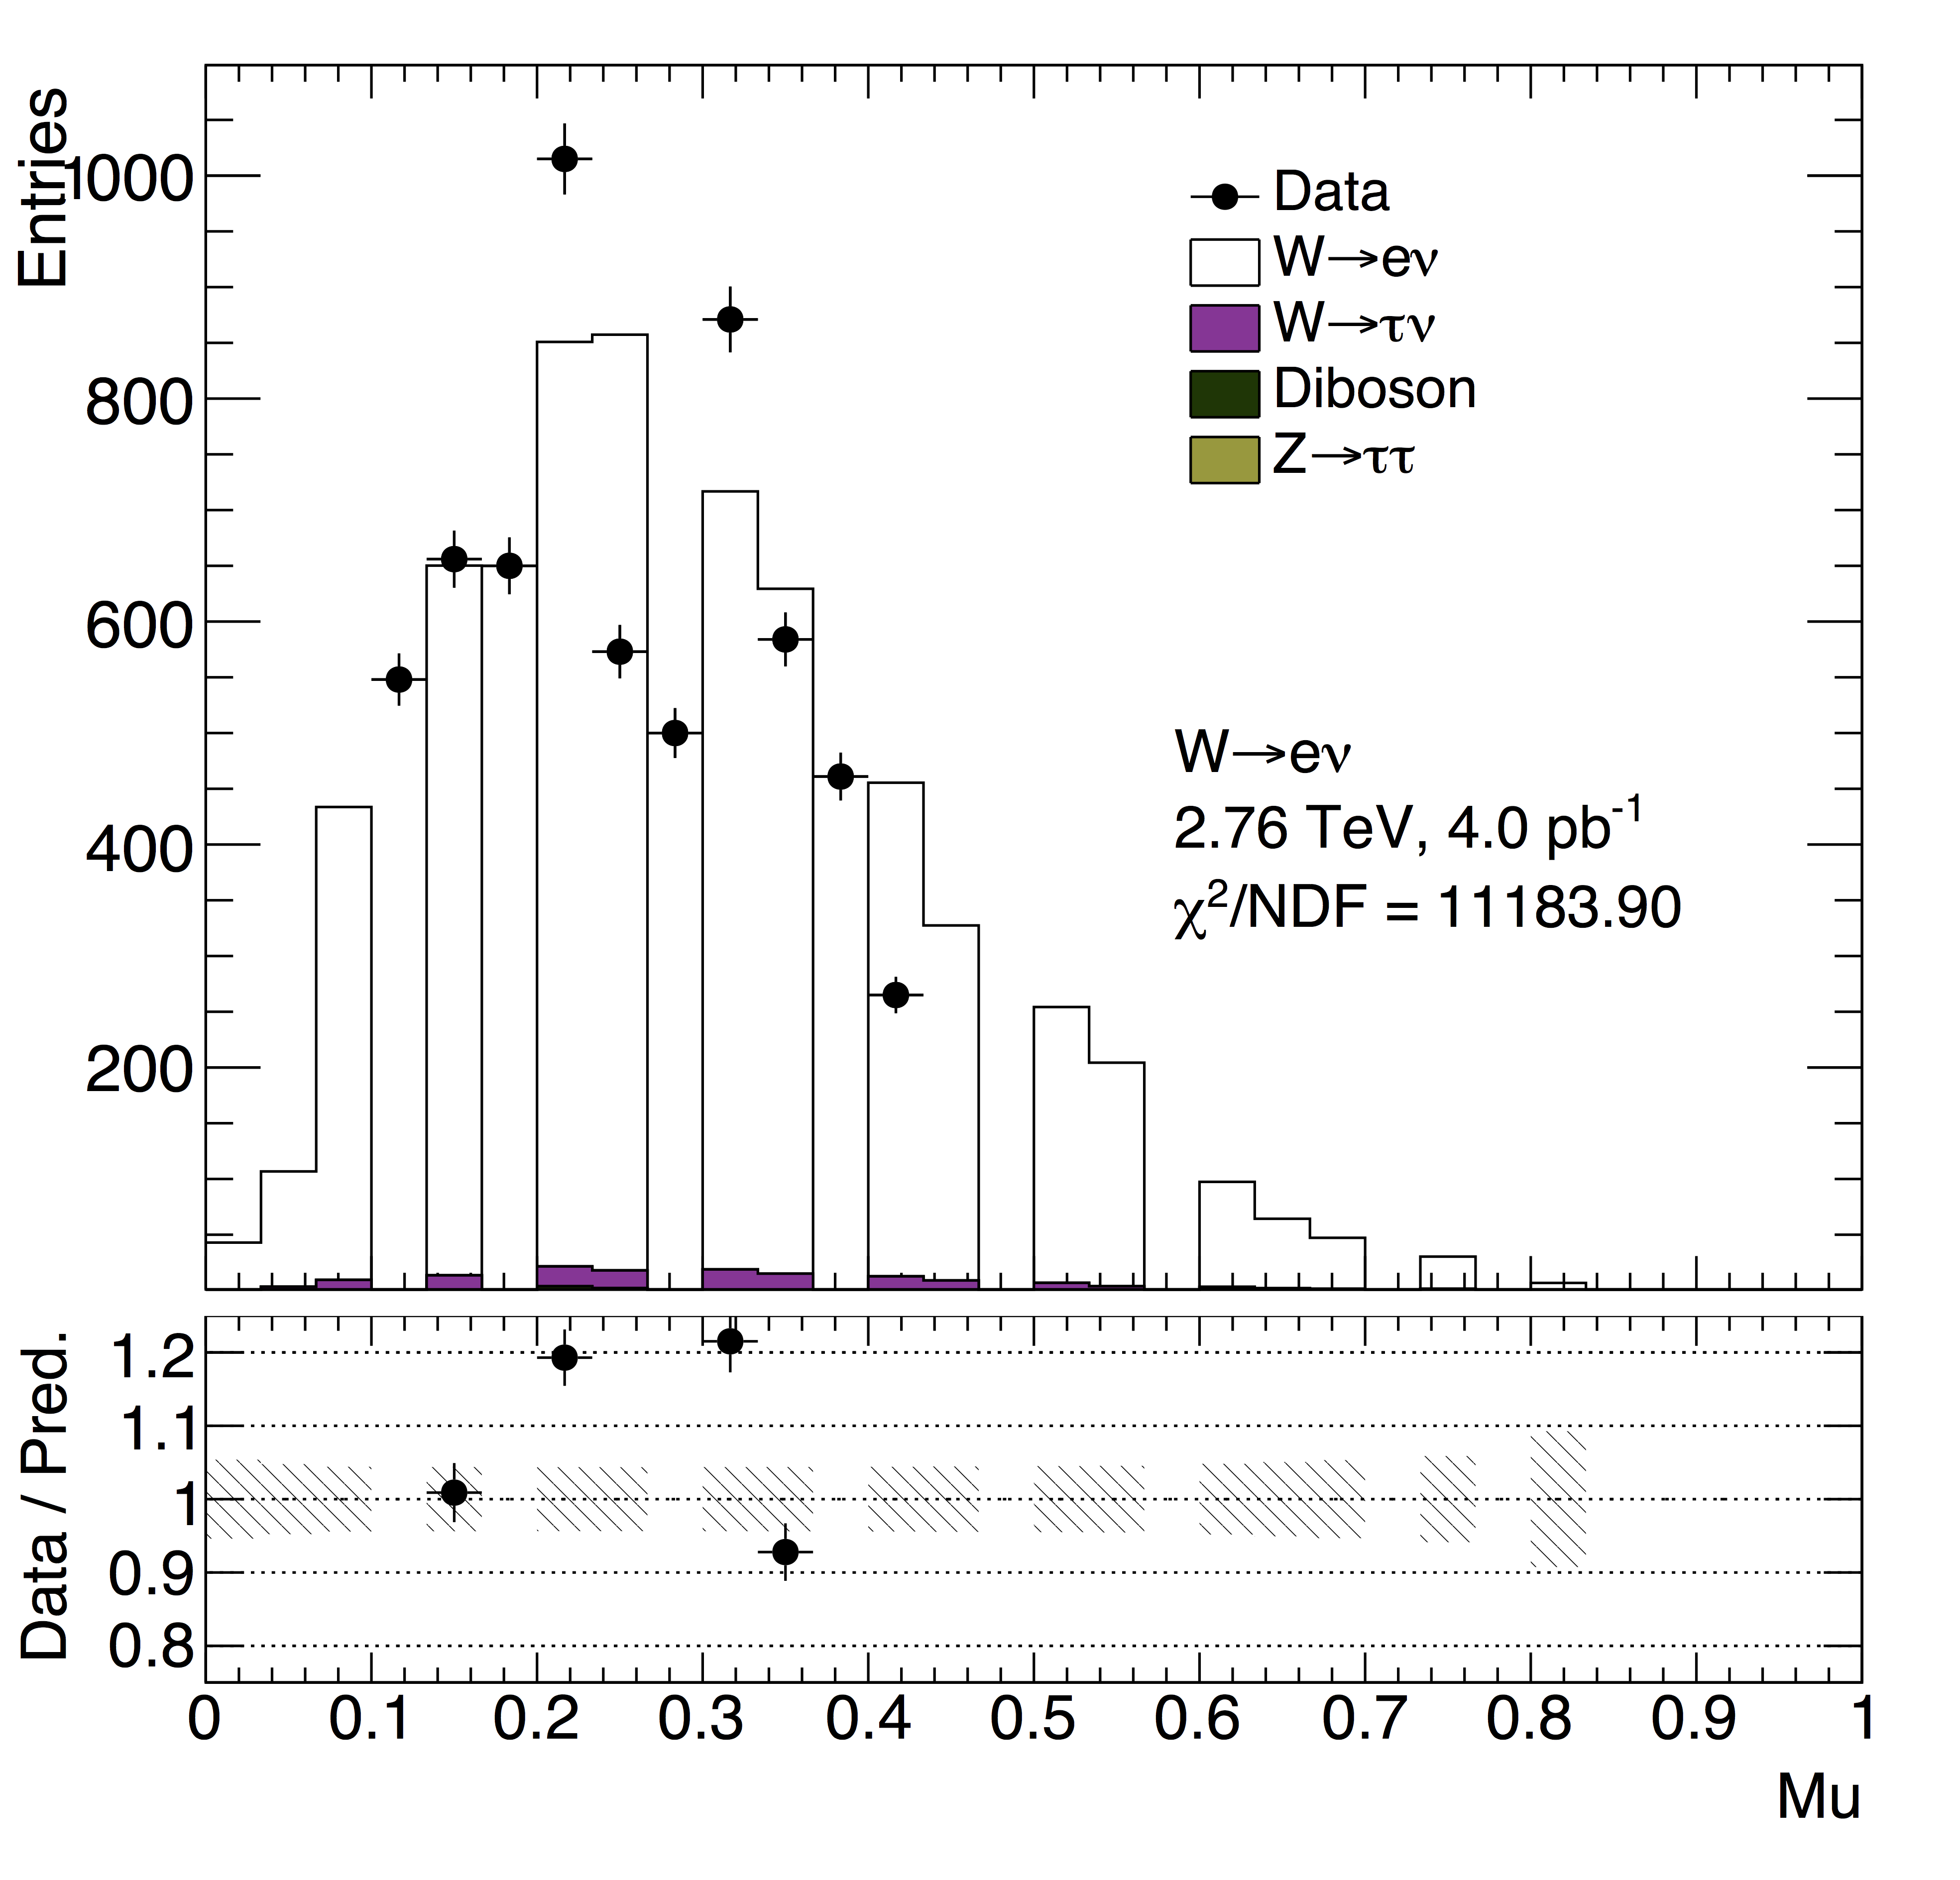
\includegraphics[width=0.5\textwidth]{HadronRecoil/W_Event_Mu.png}
\caption{Mean number of interactions per bunch crossing in \wenu events. In MC the pileup is modeled in a few bins only, that makes the application of the standard data to MC reweighting procedure not feasible.}
\label{HadrRecoil:mu}
\end{figure} 

\begin{figure}[!tbp]
\begin{center}
\begin{minipage}[h]{0.49\linewidth}
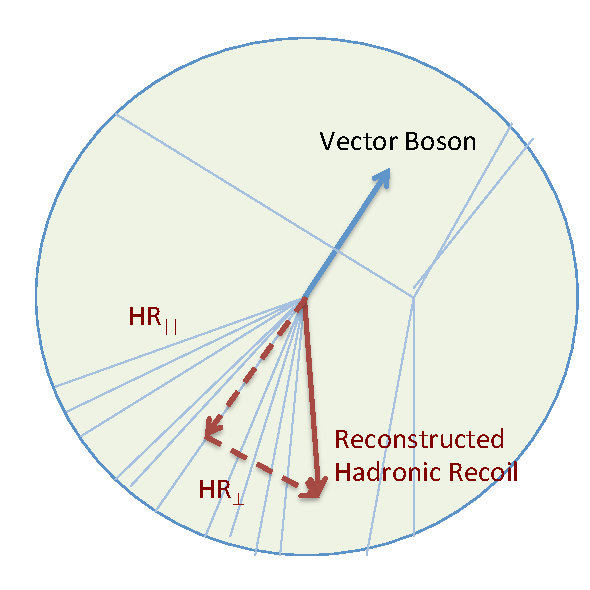
\includegraphics[width=1\textwidth]{HadronRecoil/RecoHRParPerp.pdf}
\end{minipage}
\caption{Parallel and perpendicular projections of the hadronic recoil with respect to the transverse momentum of the vector boson \cite{HRPlots}}
\label{ris:HadrRecoilTruthPt}
\end{center}
\end{figure}

This analysis uses a standard hadronic recoil calibration procedure, described in \cite{HRCorrections}, that was modified and adapted for the low statistics 2.76 TeV case. The standard procedure consist of the 3 main steps. 

The first step in the hadronic recoil calibration procedure aim to correct differences in the pile-up modeling in the event. Additional interactions can have a significant effect on \etmiss and \sumet distributions. These discrepancies are usually corrected by reweighting average number of interactions per bunch crossing in MC to match the data. However, the \atlas simulation is adjusted for high pile-up runs, so this quantity is modeled discrete in case of 2.76 TeV analysis (Fig. \ref{HadrRecoil:mu}), what makes the precise reweighting impossible. However, since the mean number is below 1, effect of these discrepancies on \etmiss distributions can be neglected. 

In the second and the third steps possible discrepancies in the resolution and the scale of the hadronic recoil are corrected. The hadronic recoil algorithm performance can be studied in MC through the projection of $\vec{HR}$ on the direction of the transverse momentum of the vector boson, as shown in Fig. \ref{ris:HadrRecoilTruthPt}. This projection can be divided into perpendicular \uperp and parallel \upar components as follows:
\begin{equation}
\upar=\vec{v_{xy}}\cdot\vec{HR}
\end{equation}
\begin{equation}
\uperp=v_x\cdot HR_y - v_y \cdot HR_x,
\end{equation}
where $\vec{v_{xy}}$ is a unitary vector along the transverse component of a vector boson momentum and $v_x$ and $v_y$ are its projections on x and y axis respectively. In the case of the true kinematics $\upar=-p_T^{bos}$ and $\uperp = 0$. However the limited calorimeter resolution is causing relatively wide distributions for these projections. The parallel component \upar is sensitive to a possible bias in the hadronic recoil, while the perpendicular \uperp can be used for determination of the resolution discrepancies. The mean and the width of these distributions can depend on different variables, such as a mean number of interactions in an event, hadronic activity, boson $P_{T}^{bos}$ etc. 

It is convenient to use Z boson decays for a hadronic recoil calibration, since its transverse momentum $P_T^Z$ can be determined not only from the hadronic recoil, but also from its decay products.  The $P_T^Z$ resolution coming from a lepton reconstruction is 3-4 times more precise, than the one extracted from a hadronic recoil. This allows to treat leptonically reconstructed $P_T^{Z}$ as a reference $P_T$ of the boson and to compare directly \uperp and \upar in the data and the MC. However, a small size of the Z sample in the 2.76 TeV data leads to a high statistics error for these distributions. 

The calibration constants can also be  derived from W boson decays. In order to exclude a possible bias from the $P_T^W$ mismodelling these calibration constants are derived through the data vs MC comparison of $P_T^{W}$ independent distributions (such as \mtw).  

In this analysis a combined procedure based on Z and W bosons decays has been used for a hadronic recoil calibration.

\begin{figure}[!t]
\begin{center}

\begin{minipage}[h]{0.7\linewidth}
\center{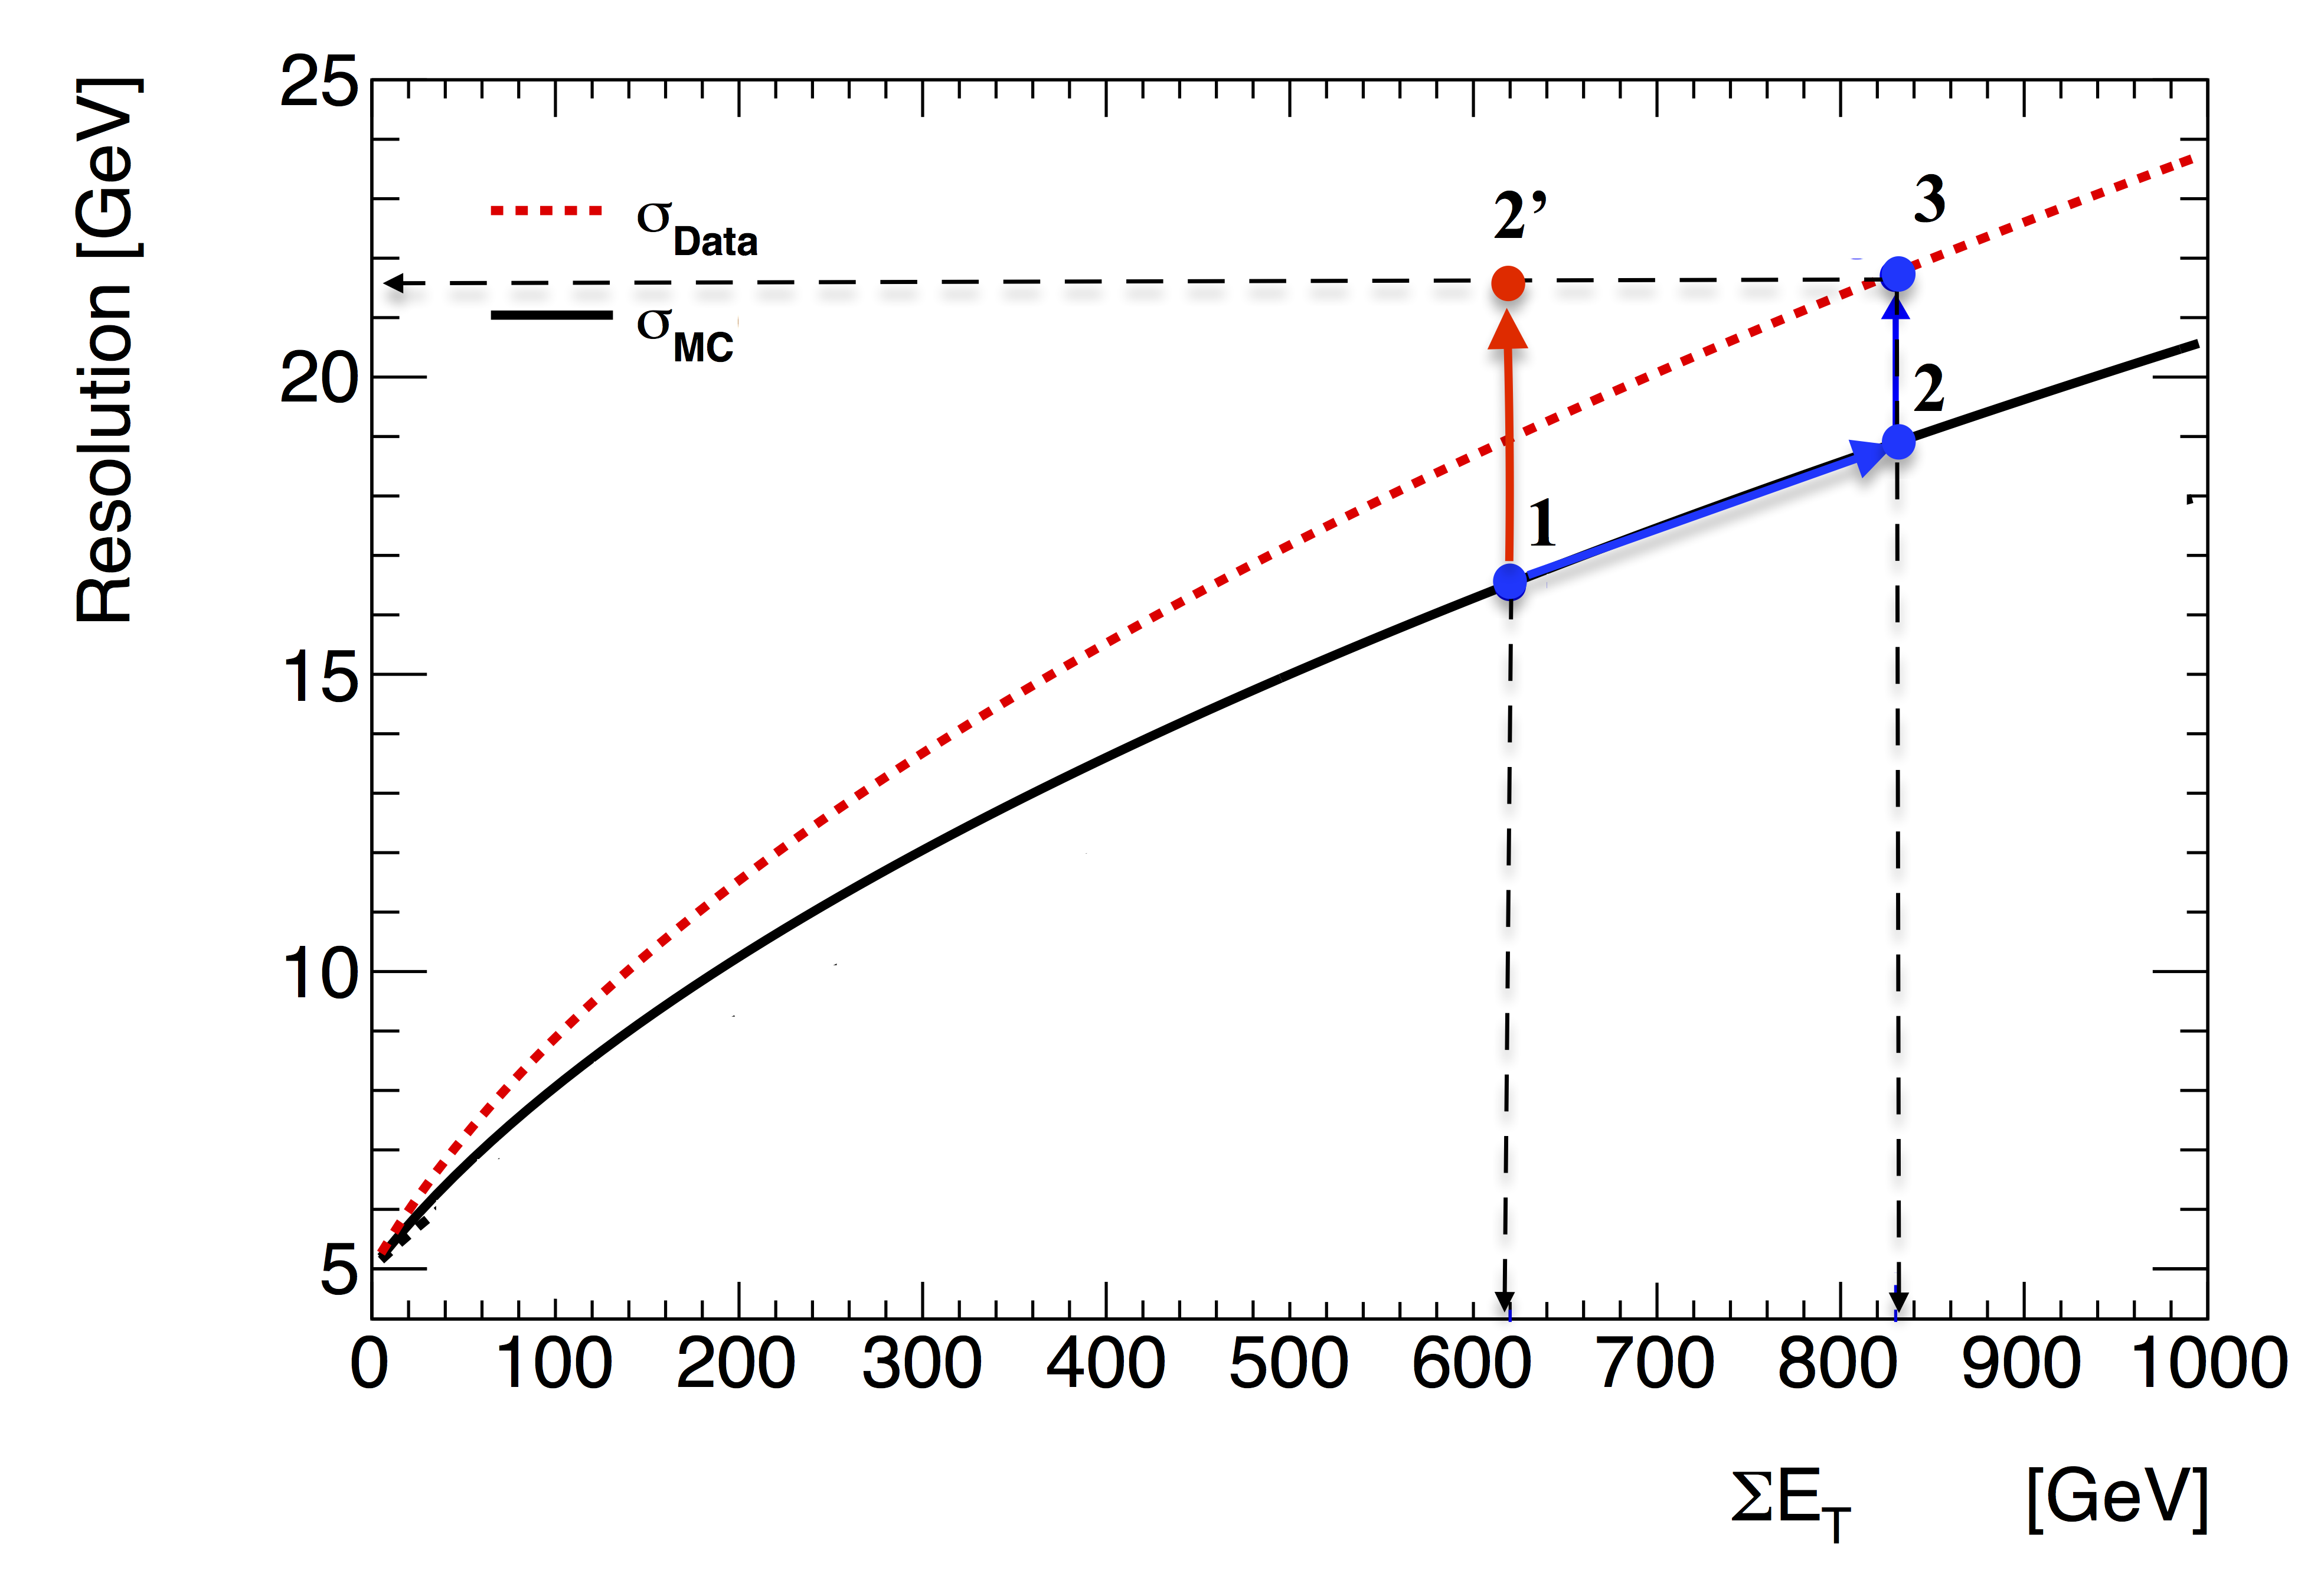
\includegraphics[width=1.\linewidth]{HadronRecoil/sumet.png}}
\end{minipage}

\end{center}
\caption{Schematic view of the correction procedure: this figure illustrates the resolution of \uperp as a function of event activity \sumet. The dotted curve represents data resolution ($\sigma_{data}$),the solid black one depicts a nominal MC resolution ($\sigma_{MC}$). Blue line from point 1 to point 2 corresponds to the \sumet correction discussed in Sec.\ref{sec:SumetCor}. The red line from point 1 to point 2' corresponds to a direct correction of the resolution mismodelling discussed in Sec. \ref{sec:ZperpSmear}. Modified from \cite{HRCorrections}}

\label{ris:sumetCor}
\end{figure}

\section{Hadronic recoil resolution correction}




The event activity plays an important role in the \etmiss reconstruction. Since \sumet and the hadronic recoil resolution values are correlated, the possible mismodelling of the event activity can lead to differences between the data and the Monte-Carlo \etmiss resolutions. There are two ways to correct the resolution in the 2.76 TeV data (Fig. \ref{ris:sumetCor}):
\begin{itemize}
\item A two step procedure, shown as path 1-2-3 in Fig. \ref{ris:sumetCor}. The first step is to correct \sumet distribution to match the data using reweighting of the events. Remaining differences in resolution are corrected at the second step. This method is discussed in Sec. \ref{sec:SumetCor}. 
\item The second order effects on \etmiss coming from \sumet modelling are neglected and the resolution differences between data and MC corrected directly. This procedure is shown as the path 1-2' in Fig. \ref{ris:sumetCor} and described in Sec. \ref{sec:ZperpSmear}.
\end{itemize}
Both of these methods have been implemented and will be described next.

\subsection{ Event activity correction}\label{sec:SumetCor}



\begin{figure}[!tbp]
\begin{minipage}[h]{0.49\linewidth}
\center{\includegraphics[width=1.\linewidth]{HadronRecoil/UncorrSumet/W_EtMiss_CorRecoilSumet.pdf} \\ a)}
\end{minipage}
\hfill
\begin{minipage}[h]{0.49\linewidth}
\center{\includegraphics[width=1.\linewidth]{HadronRecoil/UncorrSumet/Wmu_EtMiss_CorRecoilSumet.pdf} \\ b)}
\end{minipage}
\caption{Event activity \sumet distribution from a) the \wenu selection and b) the \wmunu selection. There is a clear sign of the event activity mismodelling in both channels, that should be corrected.}
\label{HadrRecoil:UncorrSumet}
\end{figure}

\begin{figure}[!tbp]
\begin{minipage}[h]{0.49\linewidth}
\center{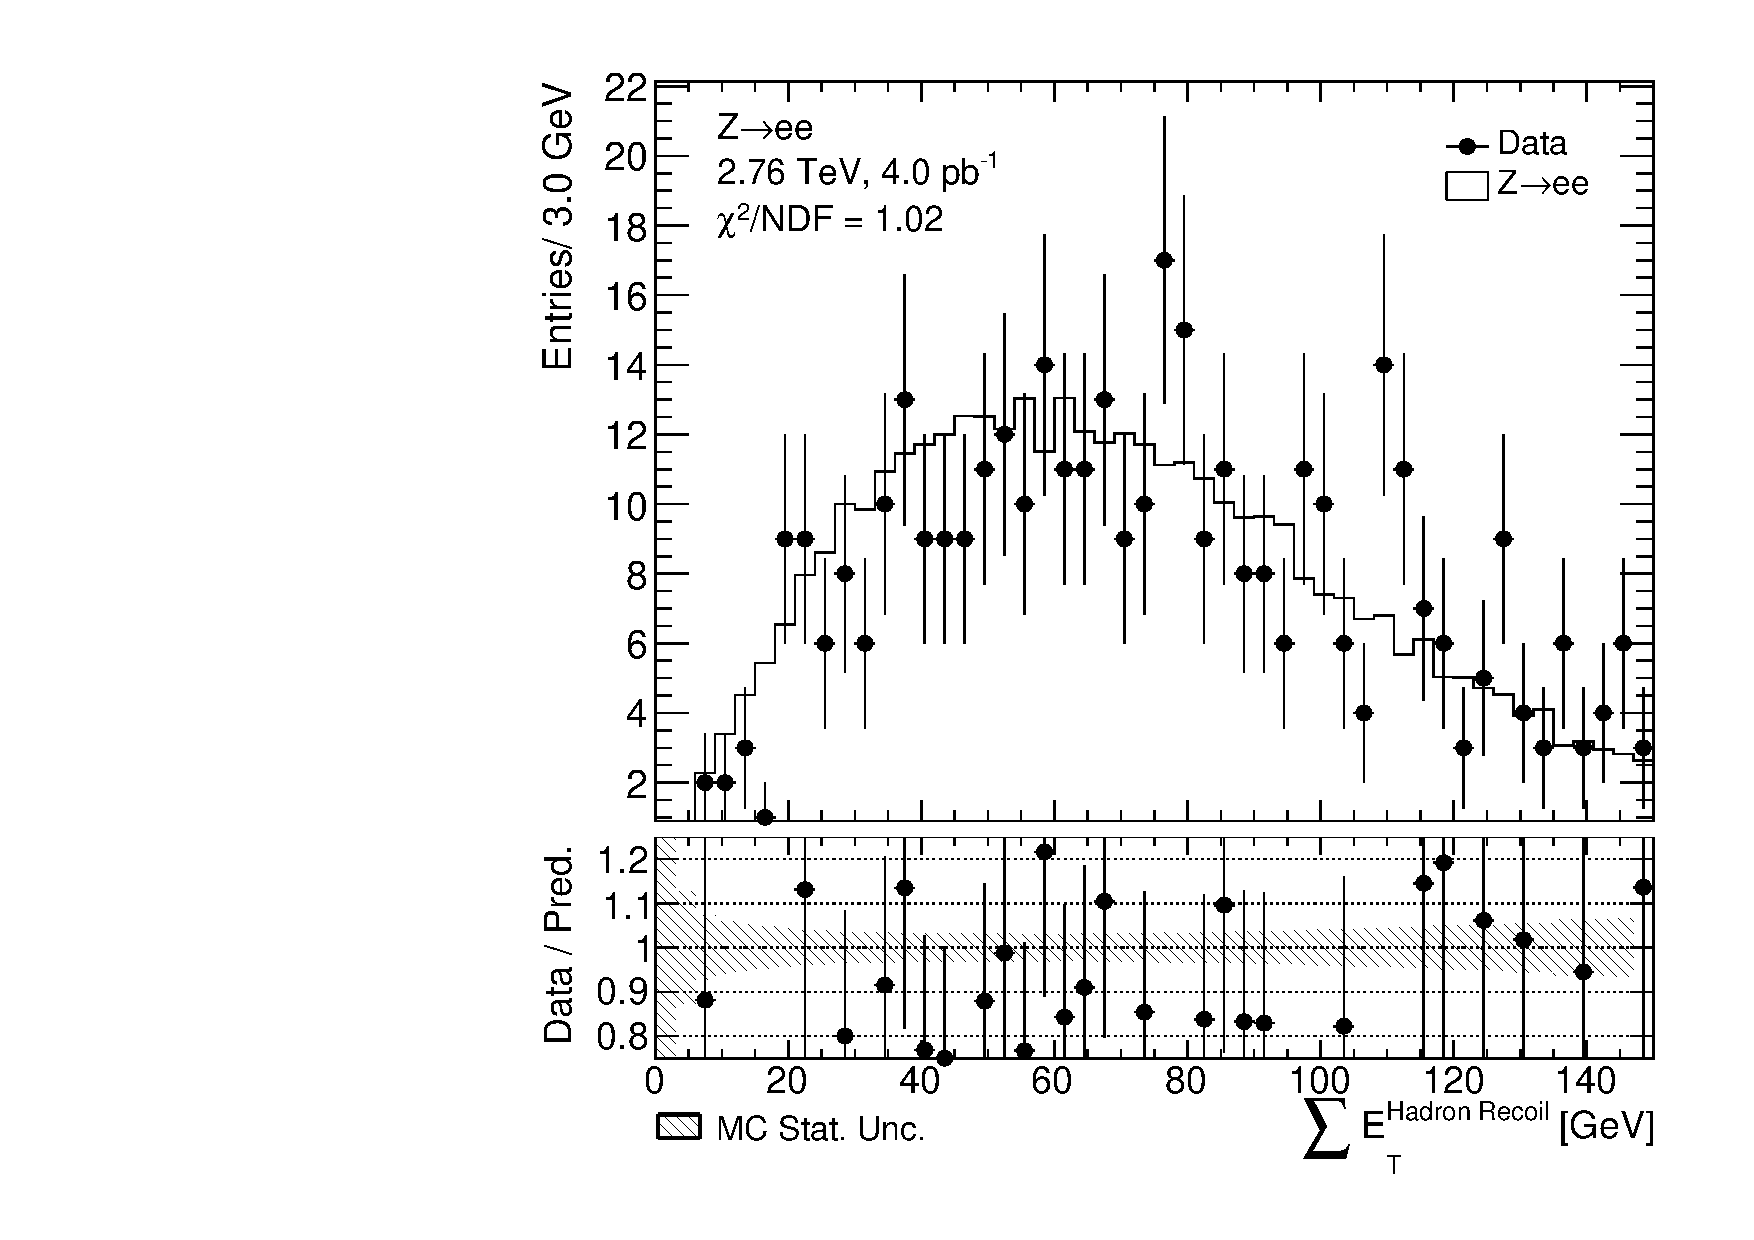
\includegraphics[width=1.\linewidth]{HadronRecoil/ZeeSumet.pdf} \\ a)}
\end{minipage}
\hfill
\begin{minipage}[h]{0.49\linewidth}
\center{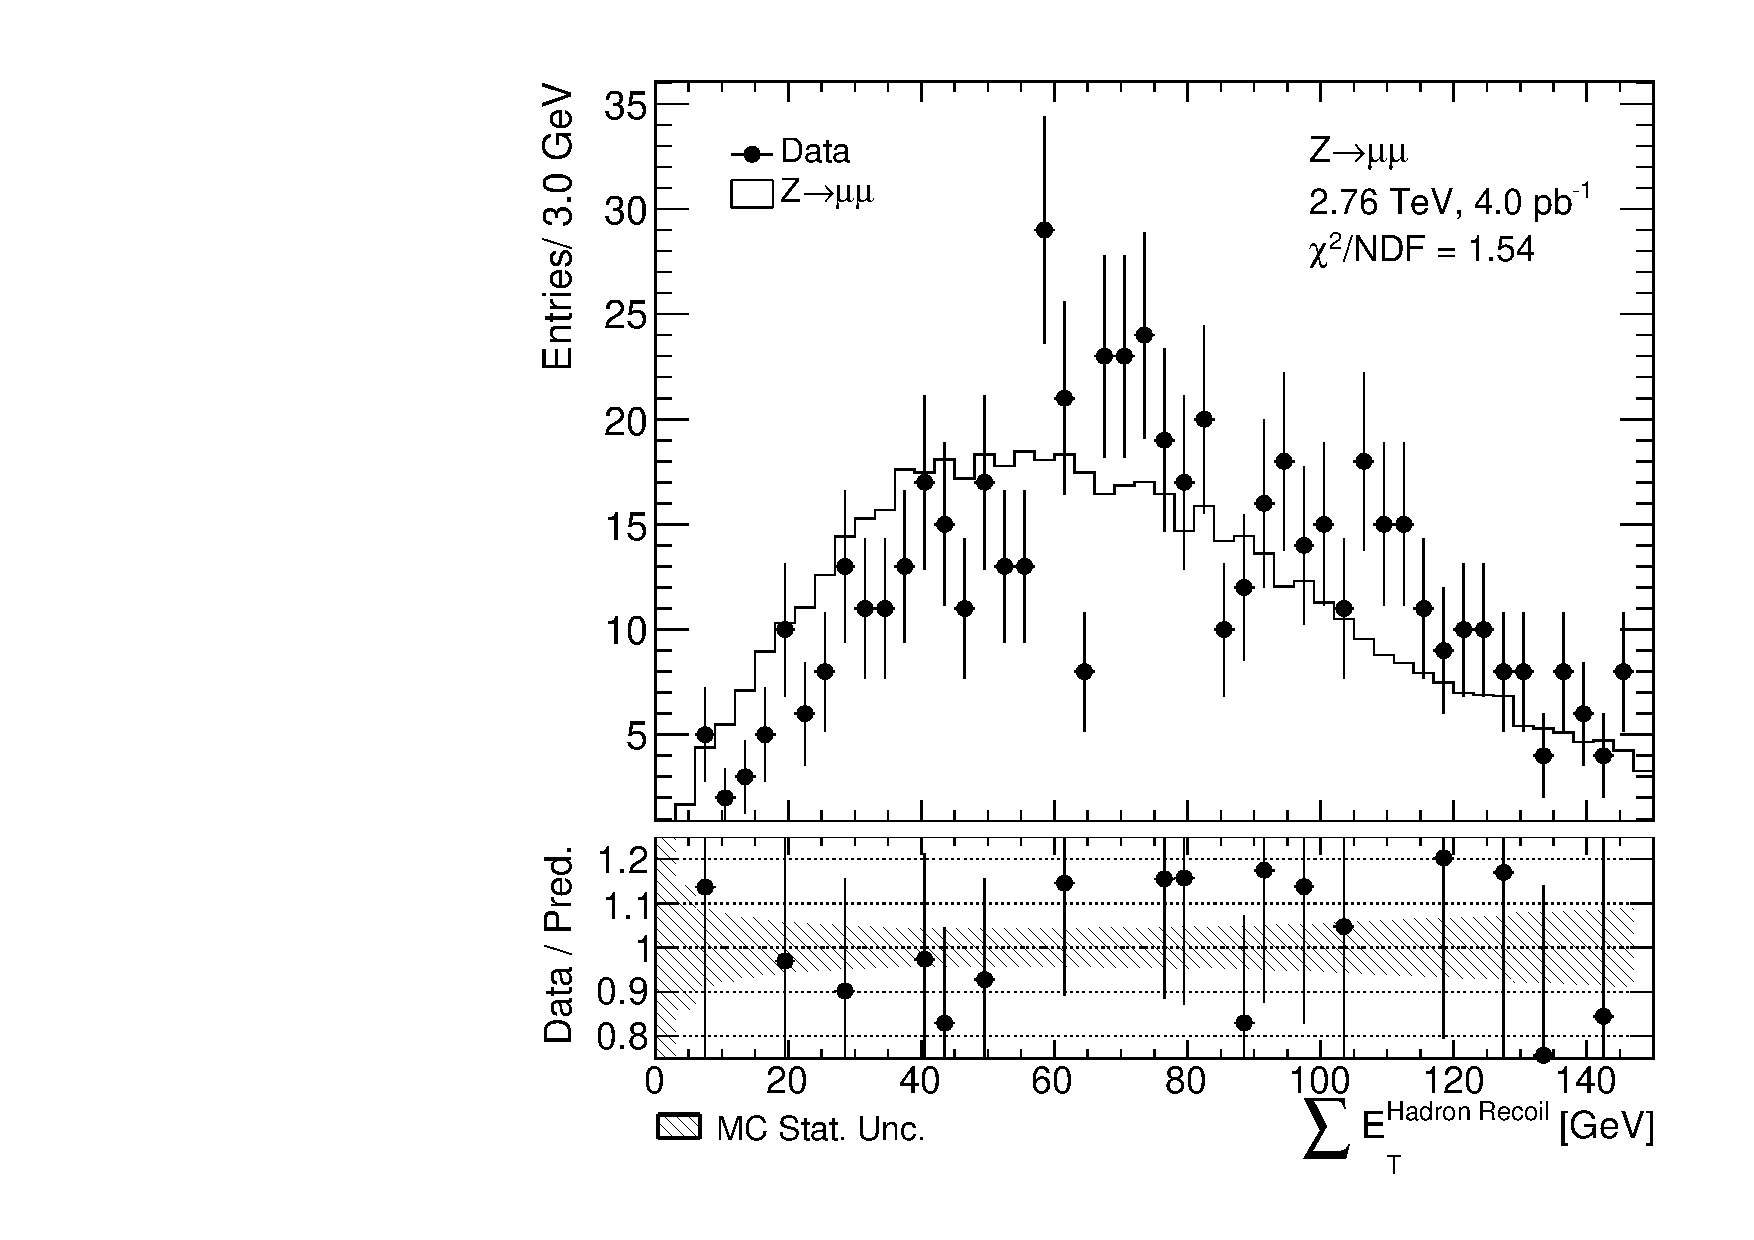
\includegraphics[width=1.\linewidth]{HadronRecoil/ZmumuSumet.pdf} \\ b)}
\end{minipage}
\caption{Event activity \sumet distribution from a) the $Z\to ee$ selection and b) the $Z\to \mu\mu$ selection. The size of the Z sample in 2.76 TeV data is insufficient correct the mismodelling of the event activity. }
\label{HadronRecoilSumetZ}
\end{figure}

\begin{figure}[!tb]
\center{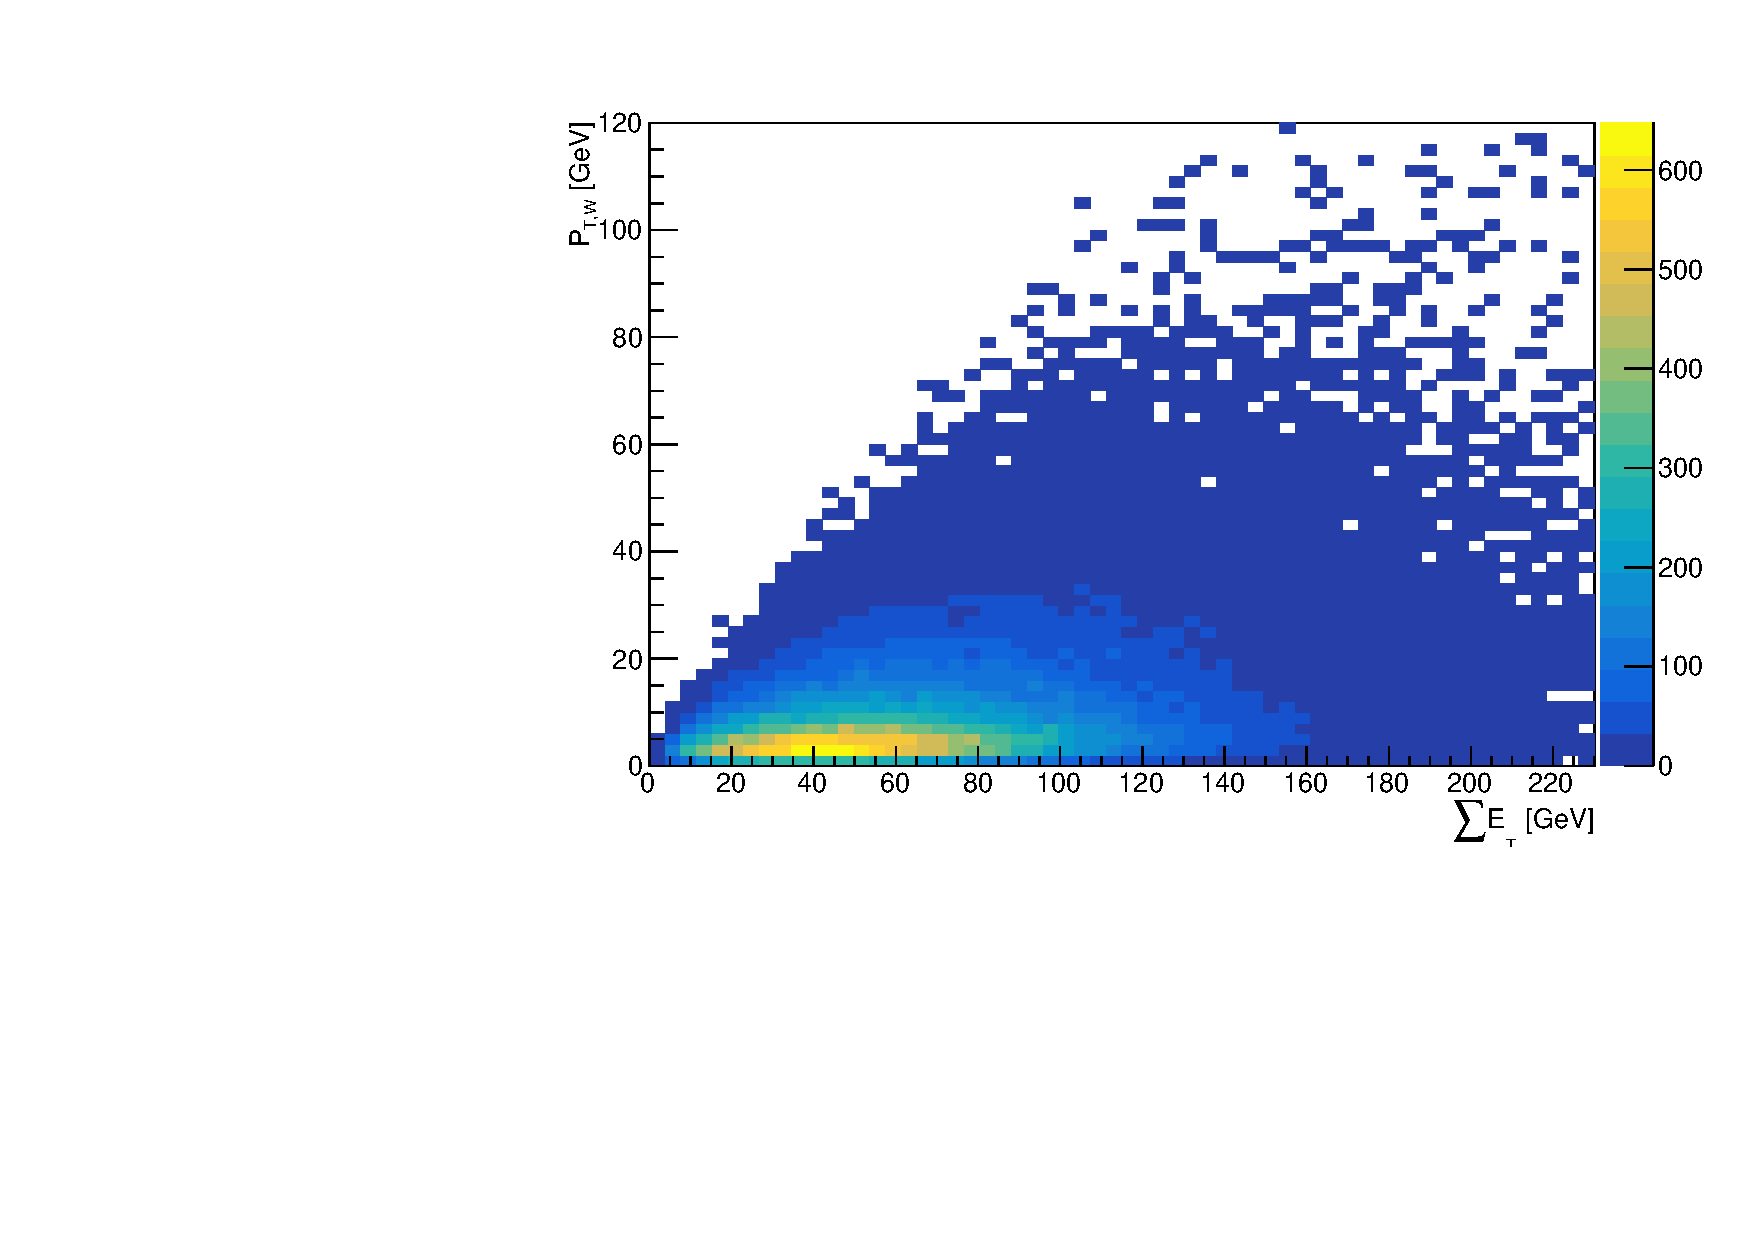
\includegraphics[width=0.9\linewidth]{HadronRecoil/SumetPtTruth.pdf} }
\caption{Distribution of event activity \sumet vs truth transverse momentum of the W boson \ptw$^{truth}$ in the $W^{+} \to e\nu$ MC sample.  }
\label{HadrRecoil:SumetPt}
\end{figure}




The distributions of the event activity \sumet  are shown in Fig. \ref{HadrRecoil:UncorrSumet}. There is a visible shift between data and the MC distribution for both W boson channels. The standard procedure, used in the \mtw measurement at 7 TeV uses a Smirnov transformation of MC, determined from the \sumet and $P_{T}^{bos}$ distributions in Z events \cite{HRCorrections}. Distribution of the event activity in the Z-boson events are shown in Fig. ~\ref{HadronRecoilSumetZ}. Since the value of $\chiD/NDF$ is around 1, it is clear that size of the Z sample is not sufficient for this procedure for both  \sumet and $P_{T}^{bos}$ distributions. This motivates a choice of the \sumet reweighting constants determination from the W-boson sample. 

\begin{figure}[!p]
\begin{minipage}[h]{0.49\linewidth}
\center{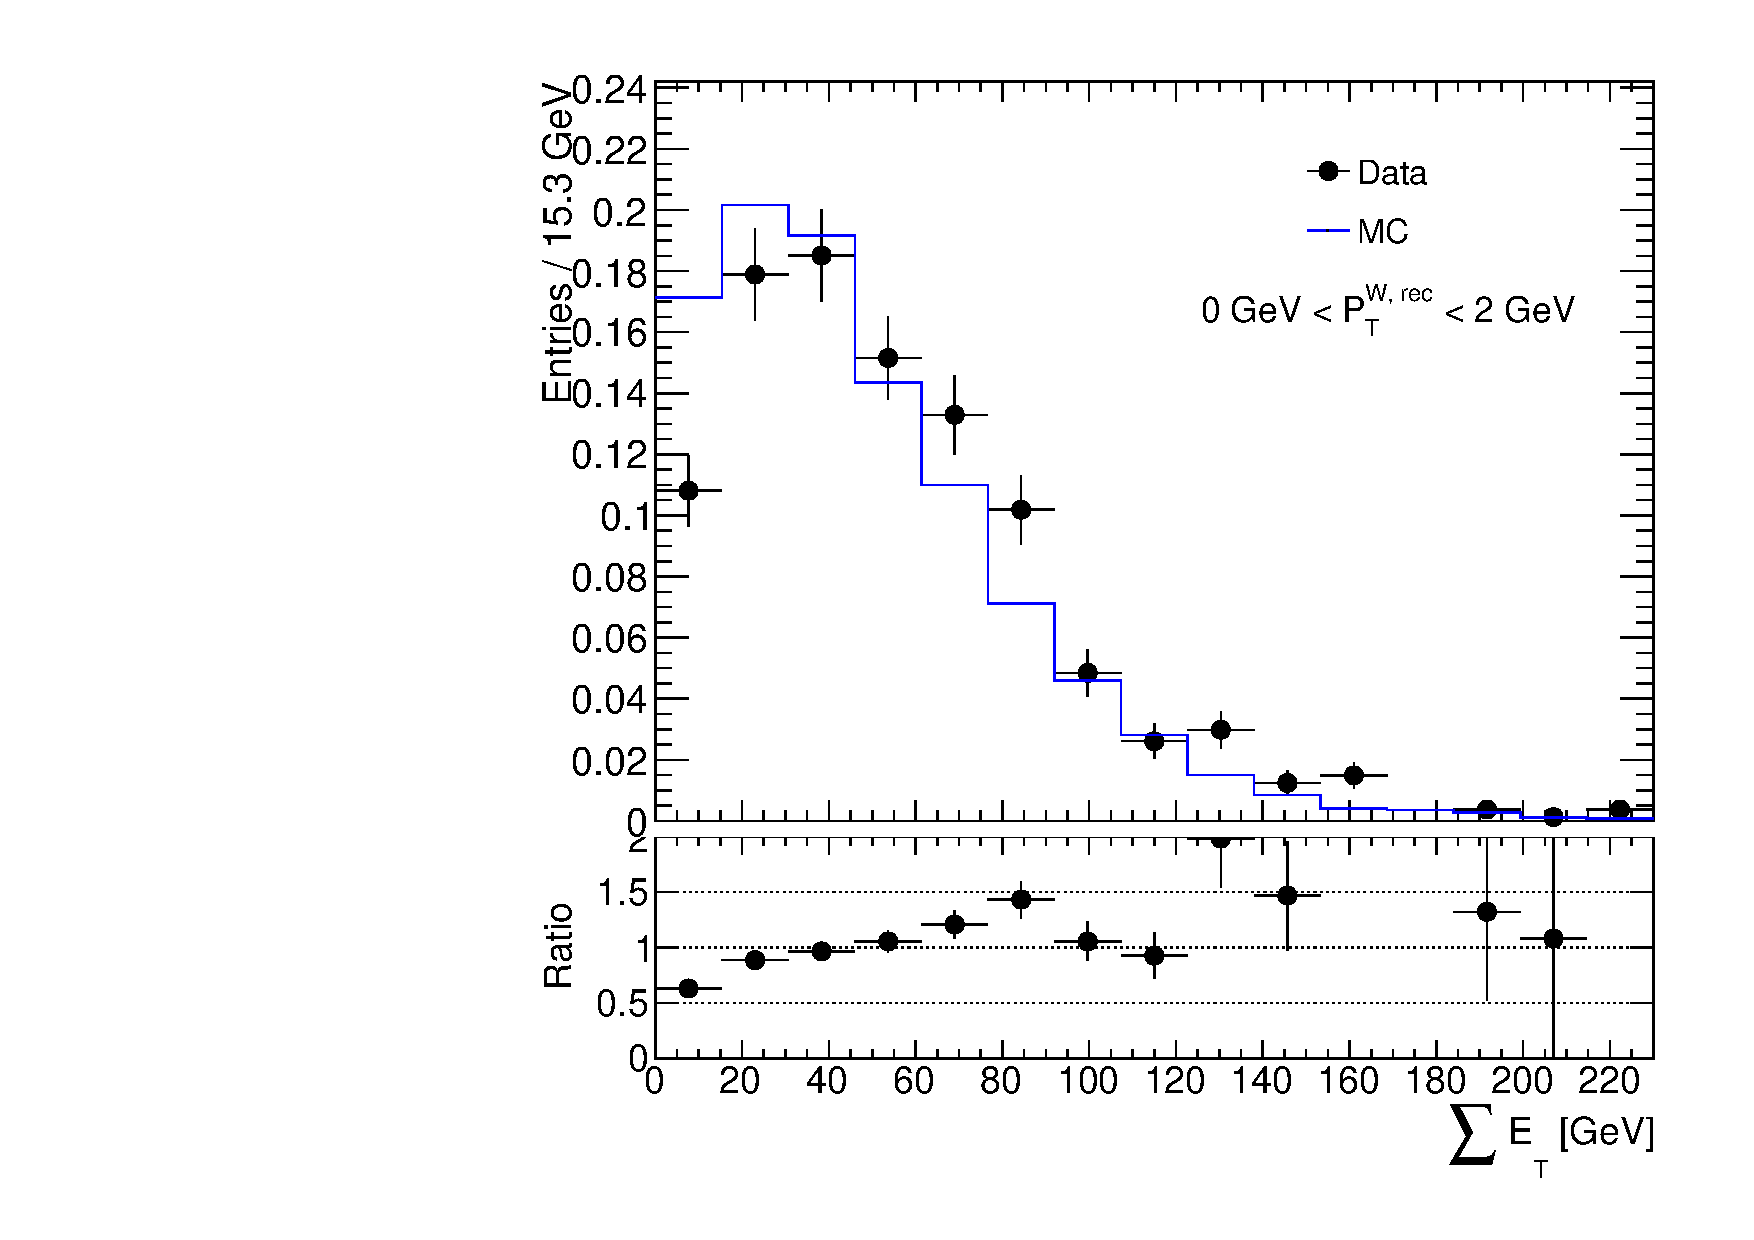
\includegraphics[width=1.\linewidth]{HadronRecoil/2.pdf} \\ a)}
\end{minipage}
\hfill
\begin{minipage}[h]{0.49\linewidth}
\center{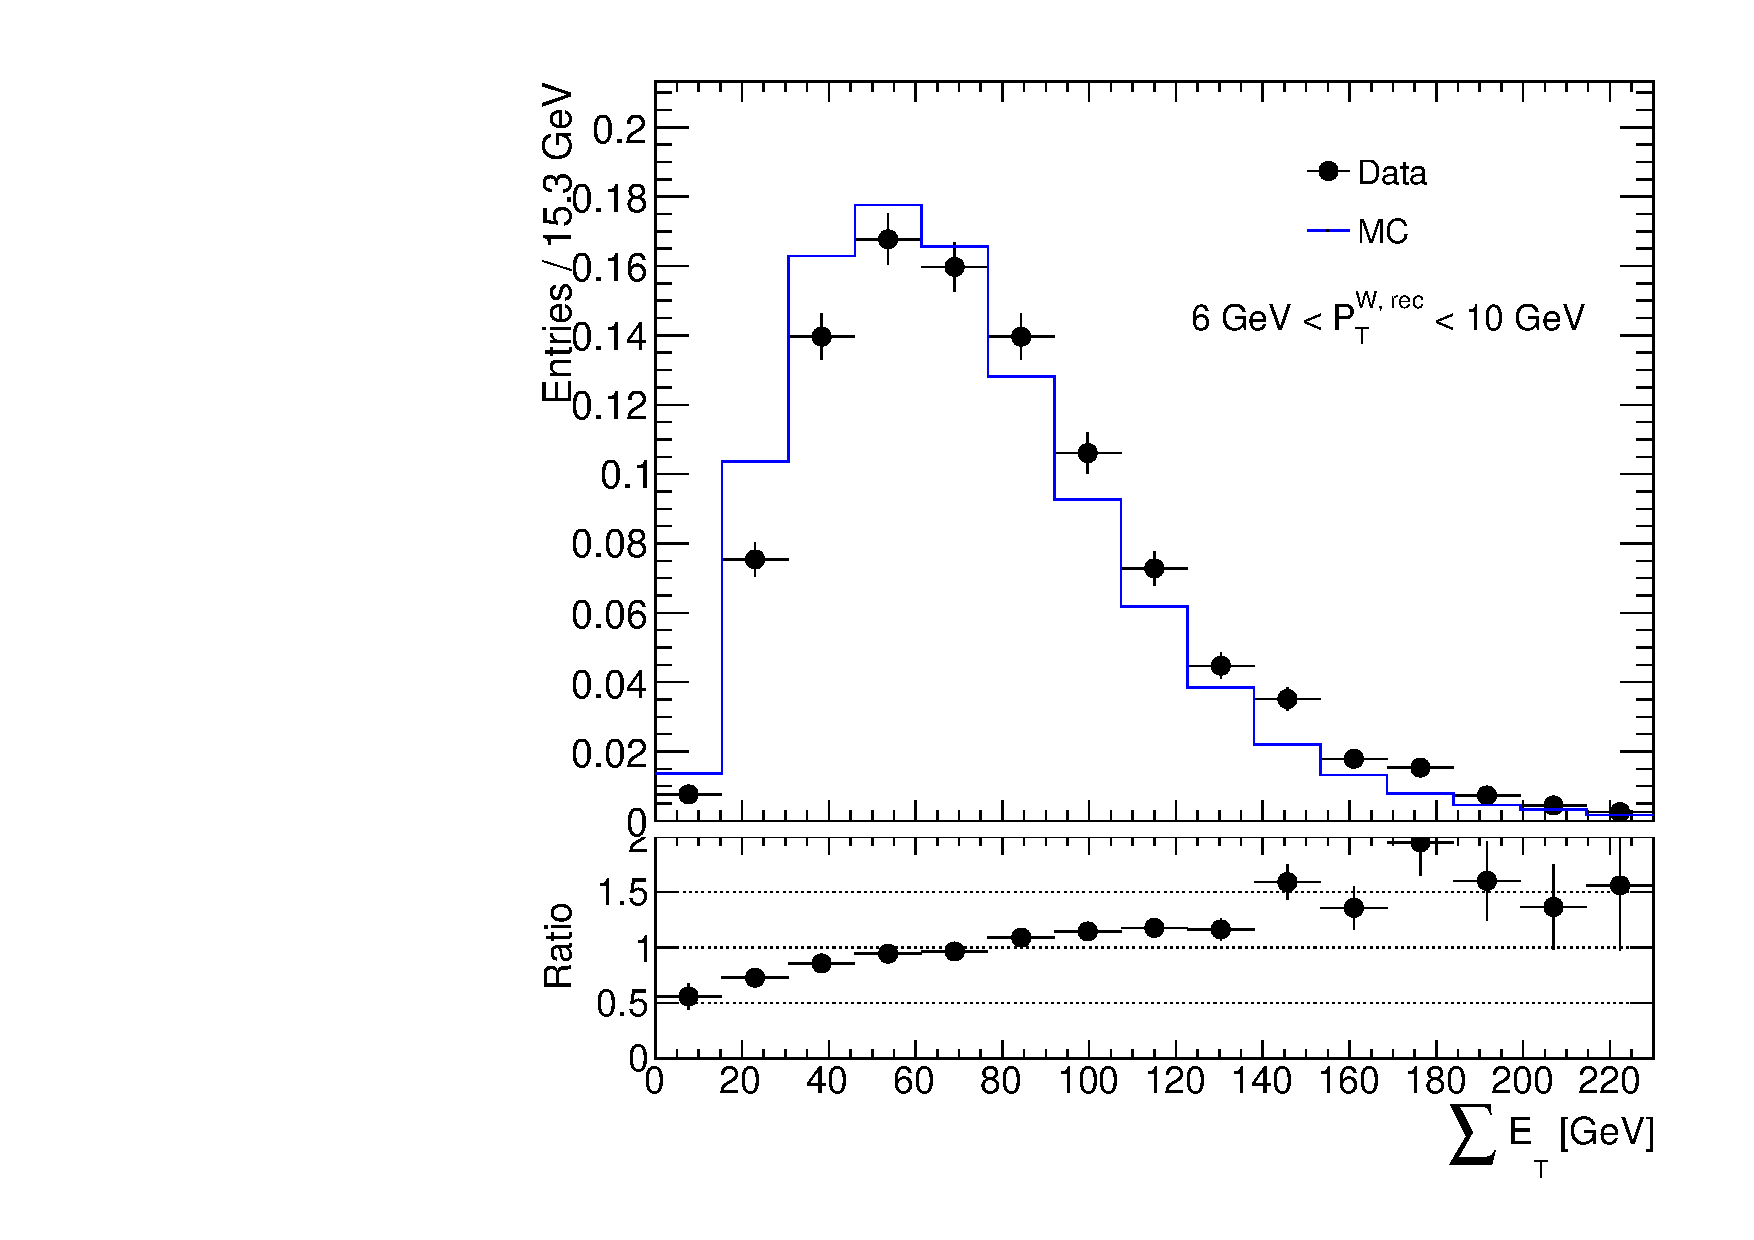
\includegraphics[width=1.\linewidth]{HadronRecoil/10.pdf} \\ b)}
\end{minipage}
\caption{Distribution of \sumet for the different $p_T^{W, rec}$ bins for $W^{+} \to e \nu$ MC sample}
\label{ris:SumEtCorPtW}
\end{figure}

\begin{figure}[!p]
\begin{minipage}[h]{0.49\linewidth}
\center{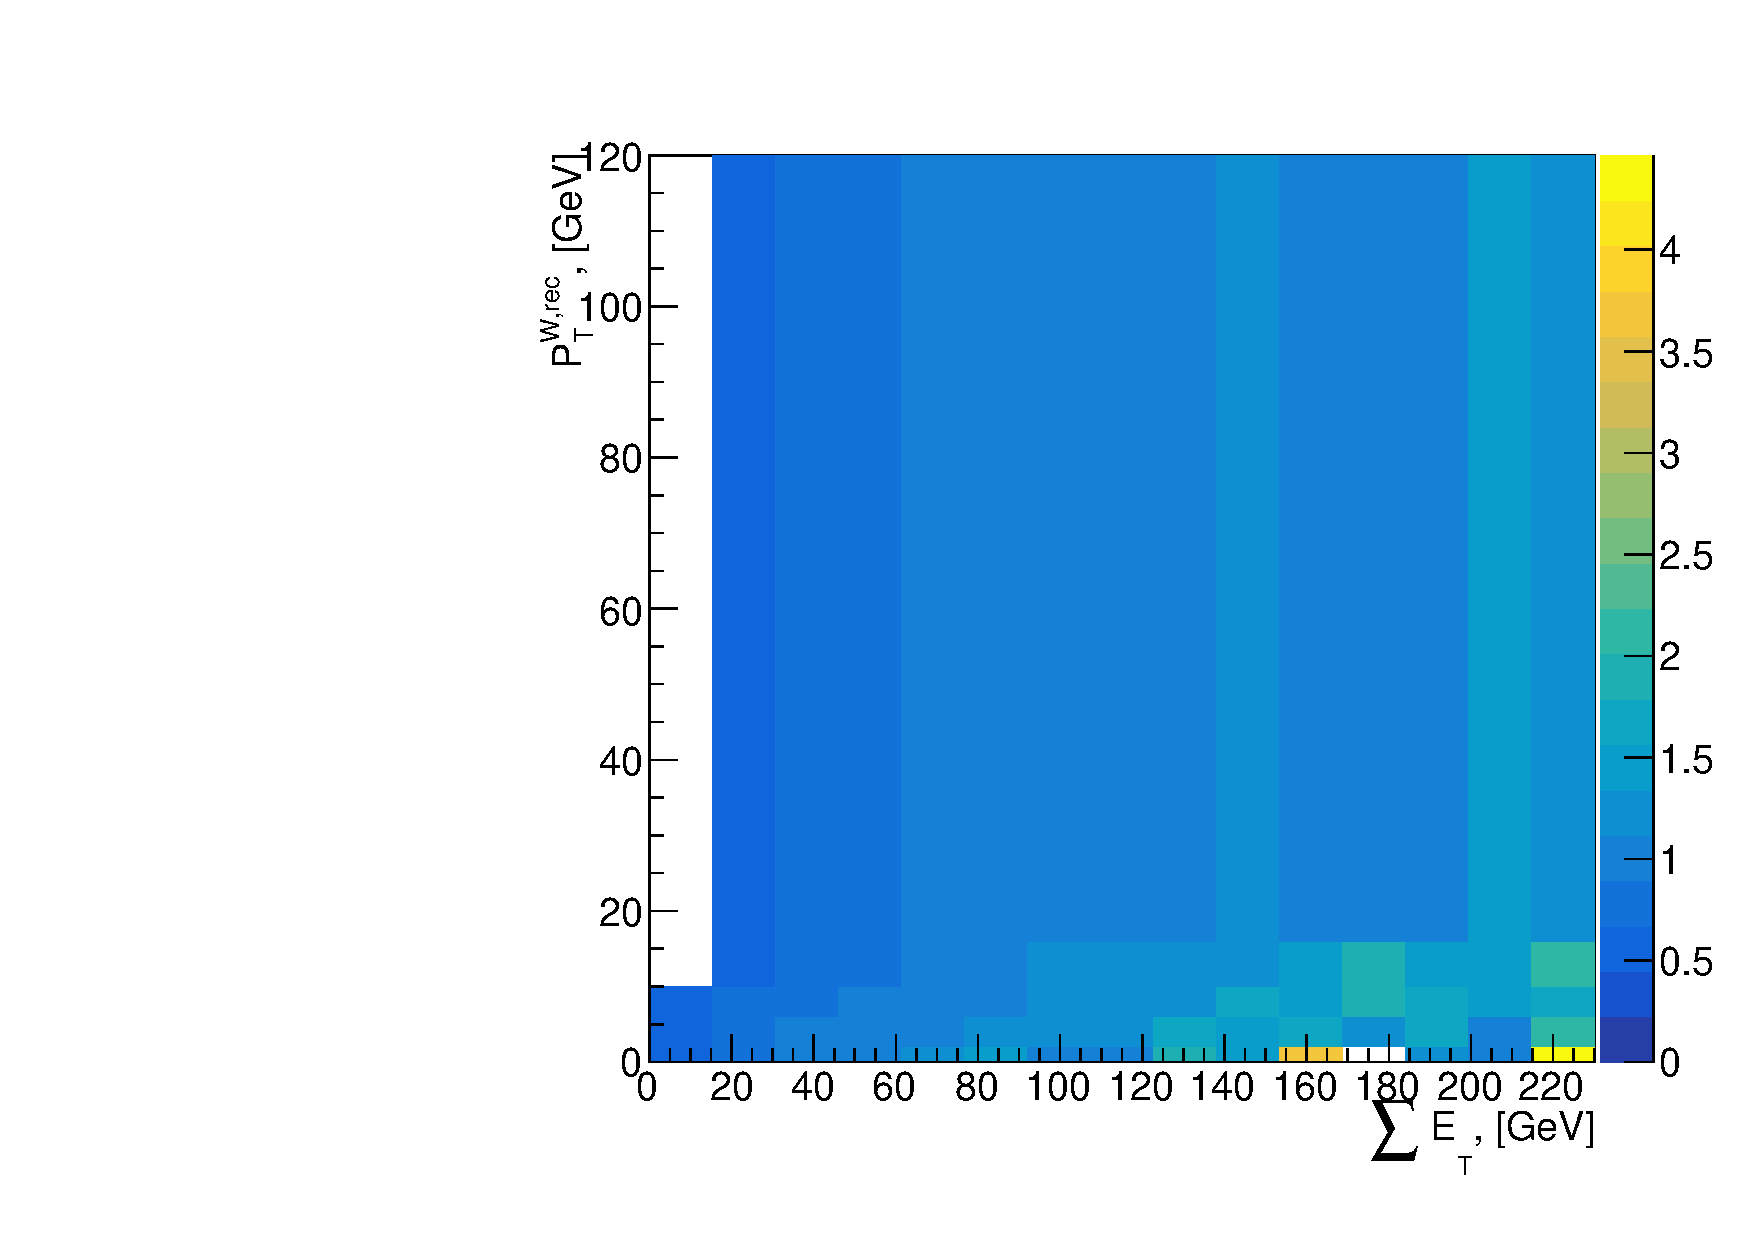
\includegraphics[width=1.\linewidth]{HadronRecoil/ReweightingNoPolEP.pdf} \\ a)}
\end{minipage}
\hfill
\begin{minipage}[h]{0.49\linewidth}
\center{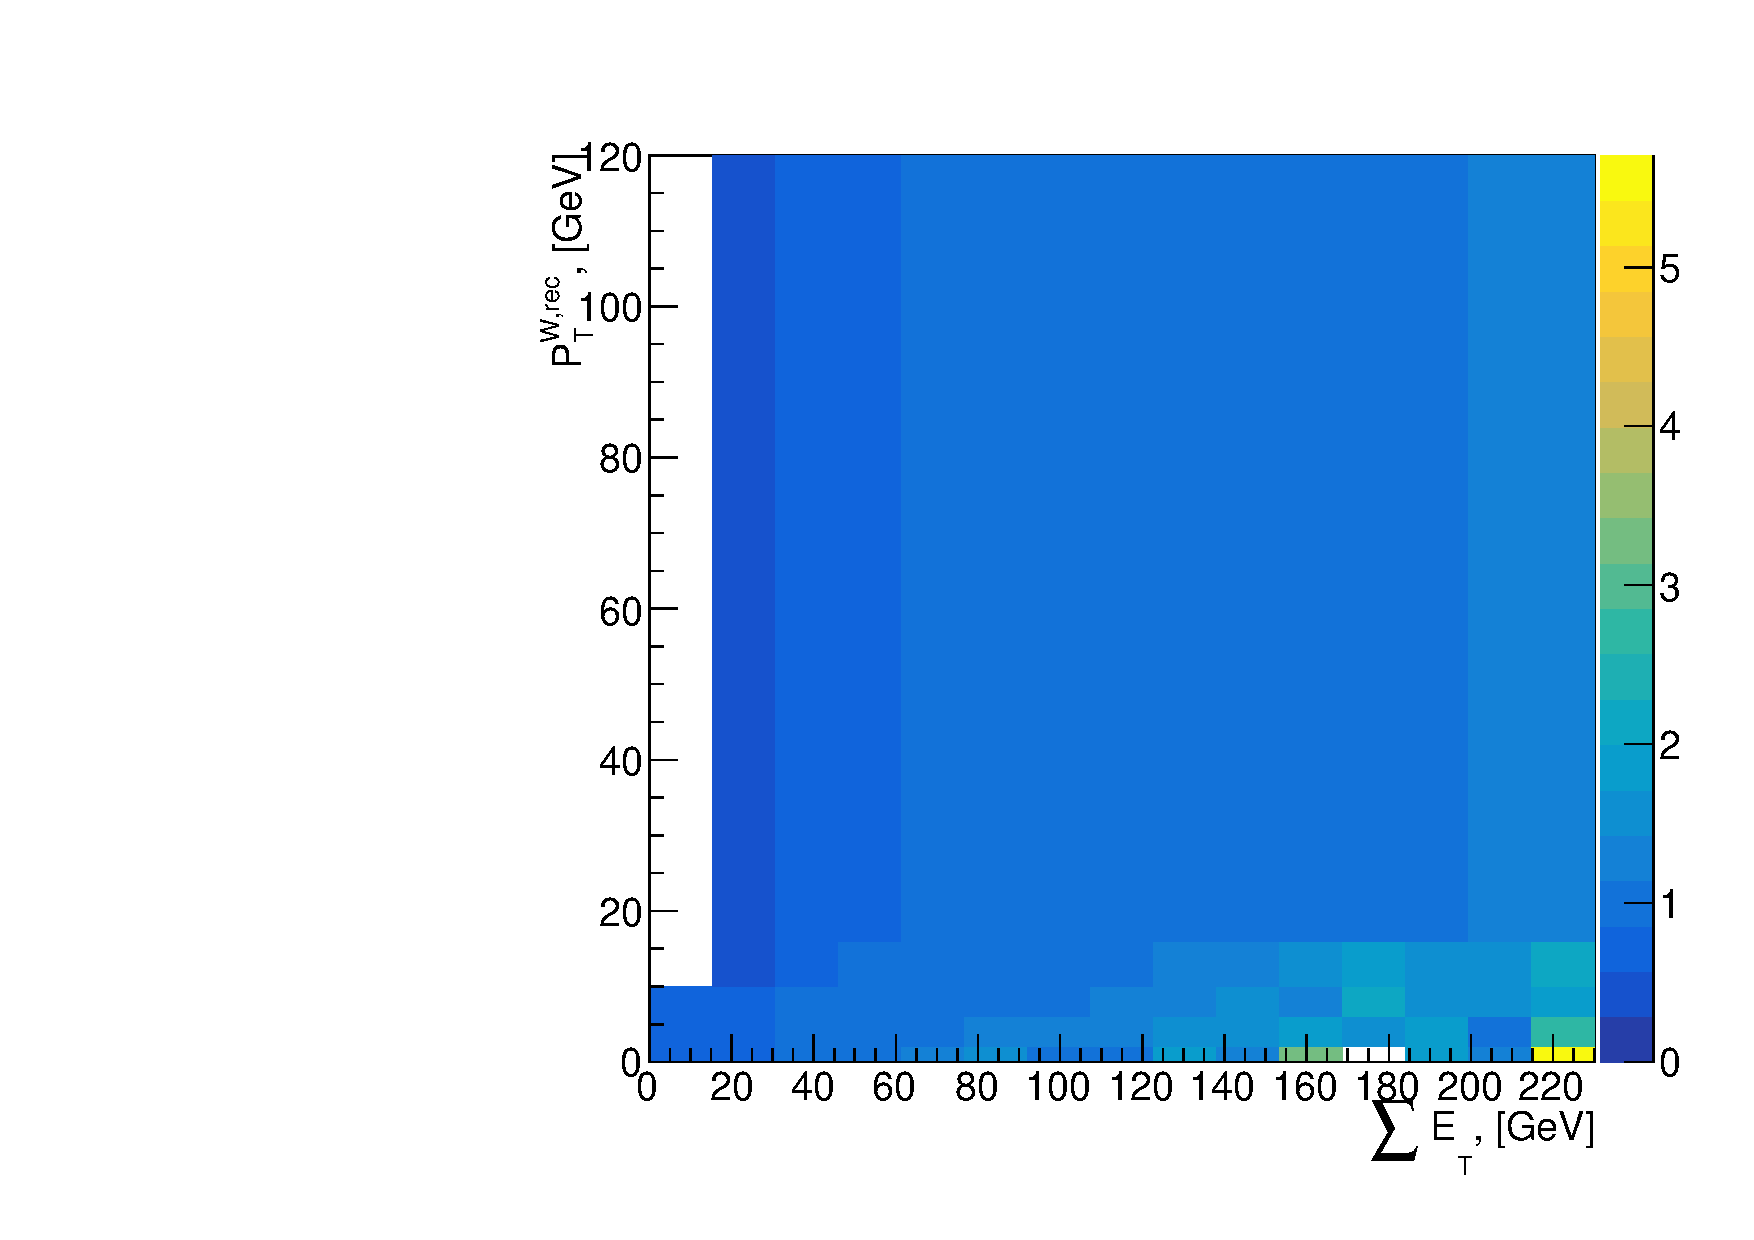
\includegraphics[width=1.\linewidth]{HadronRecoil/ReweightingNoPolMP.pdf} \\ b)}
\end{minipage}
\caption{Distribution of \sumet reweighting constants derived for a) $W^{+} \to e \nu$ and b) $W^{+} \to \mu \nu$ MC sample.}
\label{ris:SumEtCorNoPol}
\end{figure}

\begin{figure}[!p]
\begin{minipage}[h]{0.5\linewidth}
\center{\includegraphics[width=1.\linewidth]{HadronRecoil/CorrSumet/W_EtMiss_CorRecoilSumet.pdf} \\ a)}
\end{minipage}
\hfill
\begin{minipage}[h]{0.5\linewidth}
\center{\includegraphics[width=1.\linewidth]{HadronRecoil/CorrSumet/Wmu_EtMiss_CorRecoilSumet.pdf} \\ b)}
\end{minipage}
\caption{Event activity \sumet distribution from a) the \wenu selection and b) the \wmunu selection after \sumet correction. }
\label{HadrRecoil:CorrSumet}
\end{figure}

\begin{figure}[!p]
\begin{minipage}[h]{0.49\linewidth}
\center{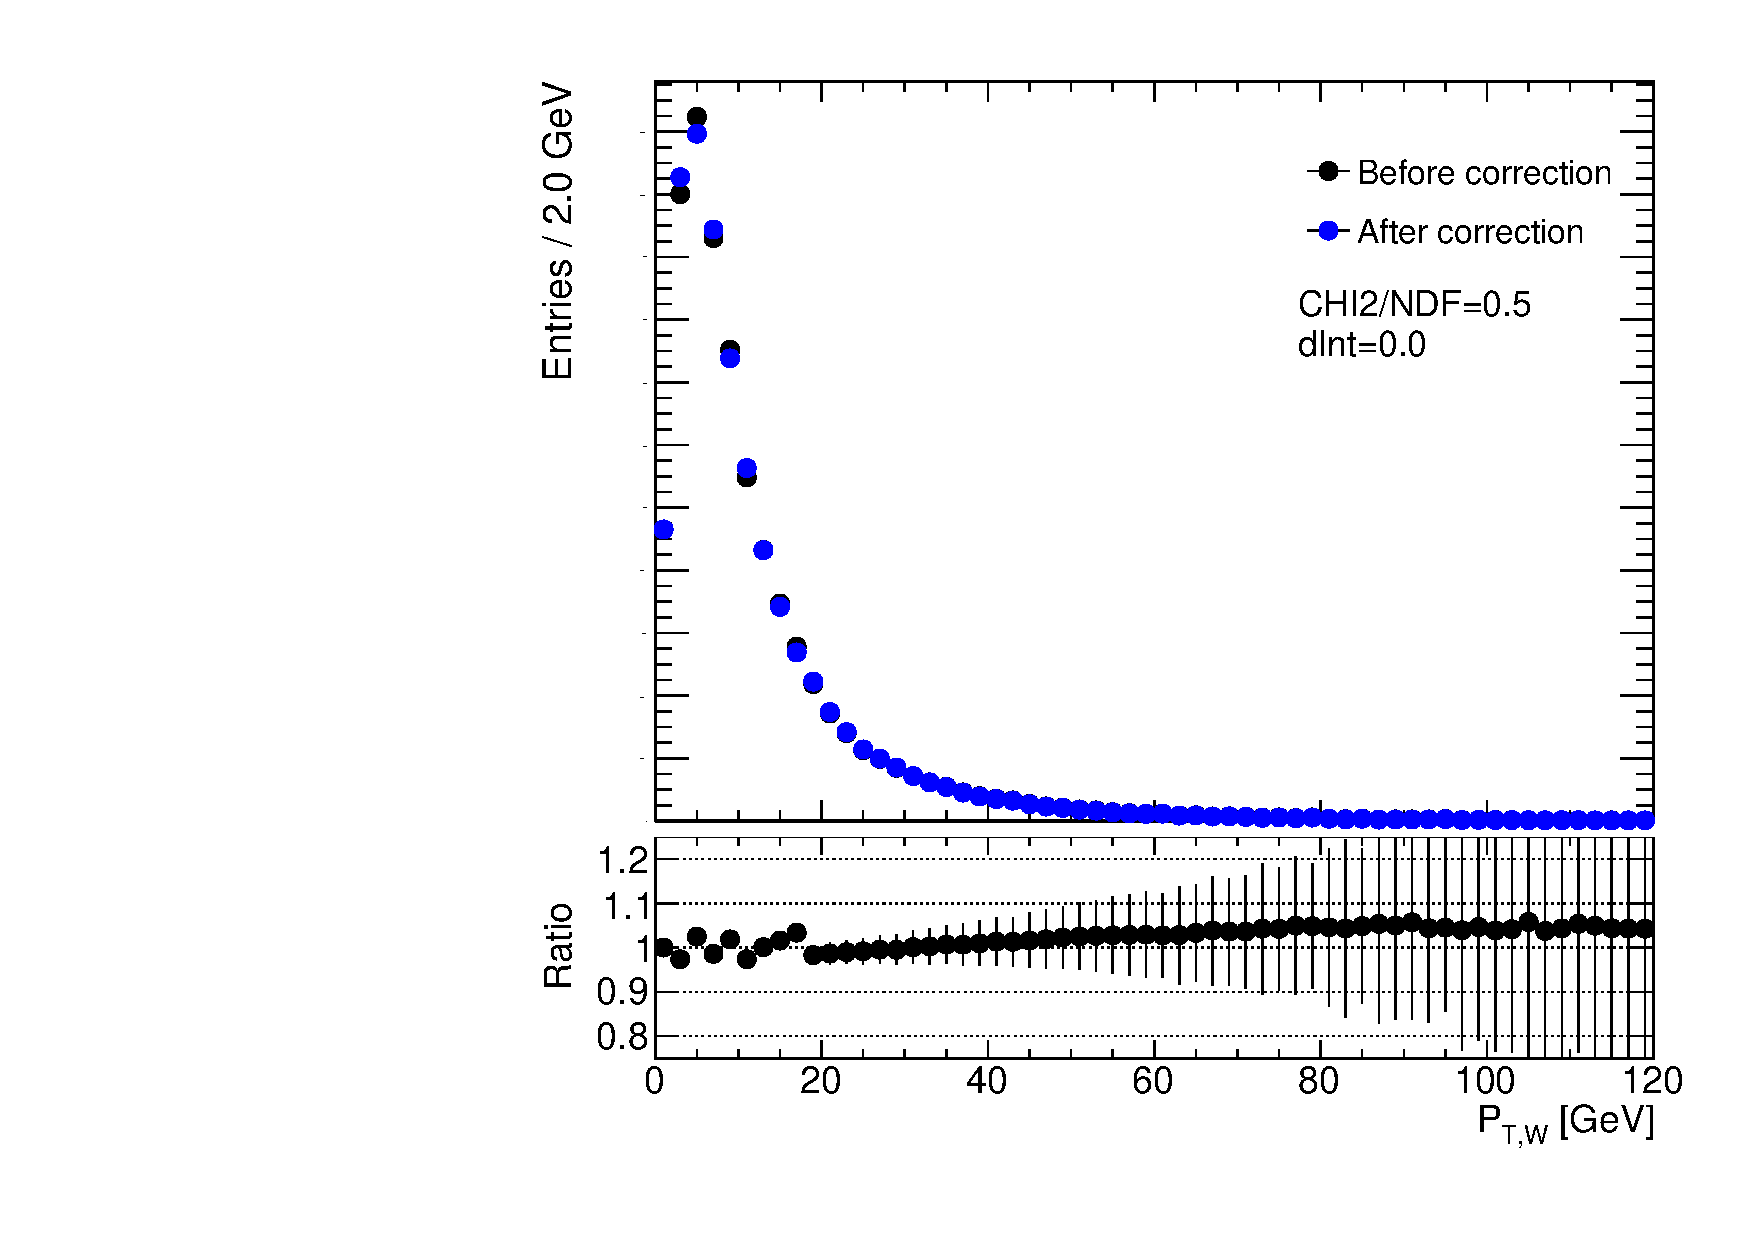
\includegraphics[width=1.\linewidth]{HadronRecoil/WplusenuRecoEffect.pdf} \\ a)}
\end{minipage}
\hfill
\begin{minipage}[h]{0.49\linewidth}
\center{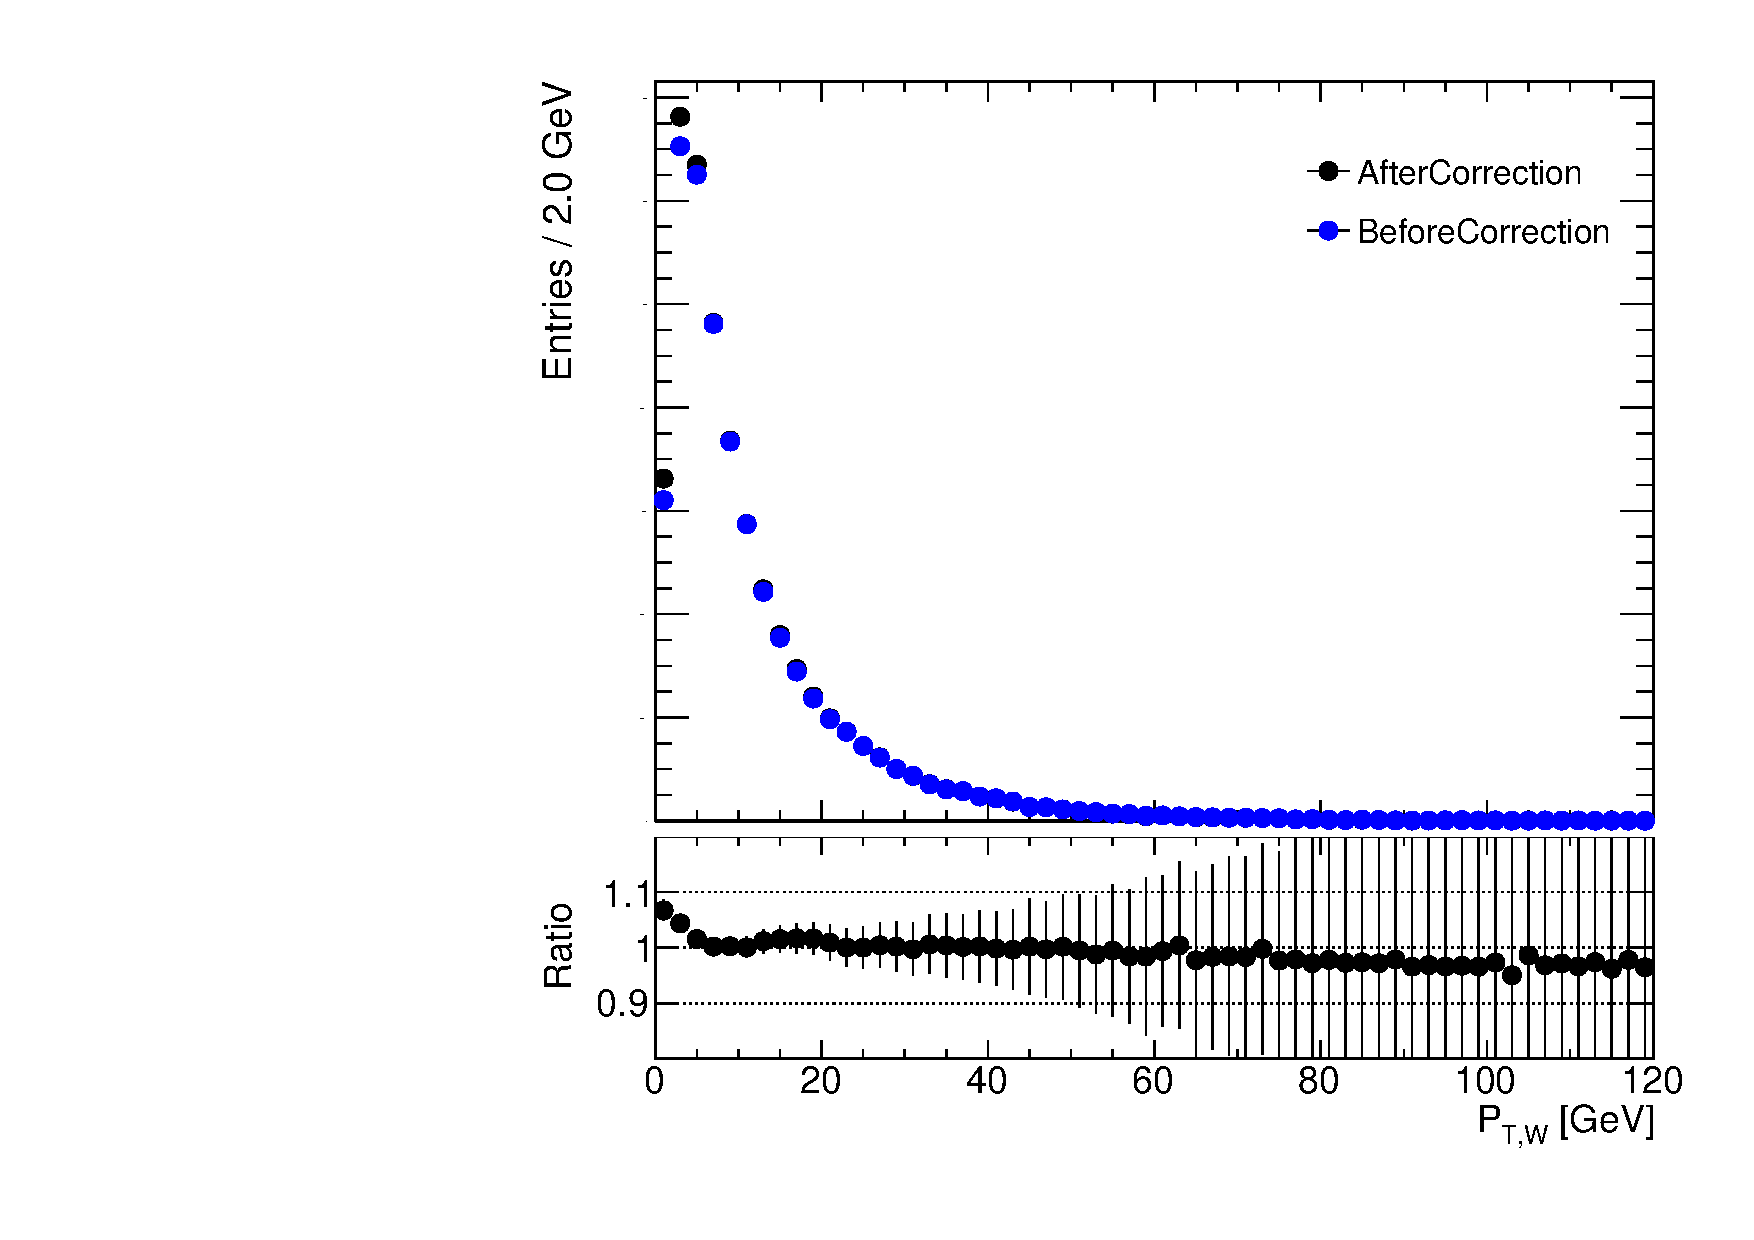
\includegraphics[width=1.\linewidth]{HadronRecoil/Wplusenu.pdf} \\ b)}
\end{minipage}
\caption{Effect of the \sumet reweighting on a) reconstructed transverse momentum of the boson and b) truth transverse momentum of the boson in $W^{+} \to e\nu$ MC sample.}
\label{HadrRecoil:PtSpectrum}
\end{figure}

The event activity \sumet is correlated to the truth transverse momentum of the boson, as shown in Fig. \ref{HadrRecoil:SumetPt}, so in order to avoid a bias from changing \ptw spectrum, reweighting constants are derived in bins of reconstructed boson momentum $P_T^{W, rec}$. Inside each $P_T^{W, rec}$ bin the reweighting constants are calculated as:
\begin{equation}
SF^{channel}=\frac{\sum E_T^{data, \, selection} }{\sum E_T^{MC,\, no\, cuts} },
\end{equation}
where $\sum E_T^{data,\, selection} $ is a \sumet distribution inside a given $P_T^{W, rec}$ after the full event selection. In order to reduce systematic uncertainty from this value, a combination of \wenu and \wmunu events is used. 

Second term $\sum E_T^{MC,\, no\, cuts}$ stands for \sumet distribution in MC before any selection. The scale factors are determined separately for each signal MC for W boson decays, in order to leave the total number of events in the the MC after the correction unchanged. Transverse boson momentum binning is chosen so that there is approximately the same number of events per bin. The total number of $P_T^{W, rec}$ bins is 6. The scale factor are applied as a reconstructed weight on MC.

The correction factors for two example $P_T^{W, rec}$ bins are shown in Fig.\ref{ris:SumEtCorPtW}. Resulting reweighting constants for \wenu and \wmunu MC samples are shown in Fig. \ref{ris:SumEtCorNoPol}. This method allows to leave the reconstructed transverse momentum of the boson nearly unmodified and introduces only a small change in a the truth boson spectrum, as shown in Fig. \ref{HadrRecoil:PtSpectrum}. 

There are two possible sources of the uncertainties of this correction: systematical, coming from the method itself and a statistical, coming from the limited data statistic. The methods of their determination and an effect of the correction on $C_{W}$ factors will be discussed.

\subsubsection{Systematic error estimation}

Systematic error on this reweighting can be estimated approximating the data to MC ratio as a function of \sumet inside each $P_T^{W, rec}$ bin with a polynomial degree 2 or 1. This method allows also to neglect effects of the data fluctuations, especially for the high \sumet regions with low statistics, as it could be seen in Fig. \ref{ris:SumEtCorNoPol}. Because of the low statistics for \sumet > 220 GeV the ratio in the last bins has been set to 1 and this region haven't been included in the polynomial fit. The total reweigting constants obtained from this procedure are shown in Fig. \ref{ris:SumEtCorPol}. 

\begin{figure}[!tbp]
\begin{minipage}[h]{0.49\linewidth}
\center{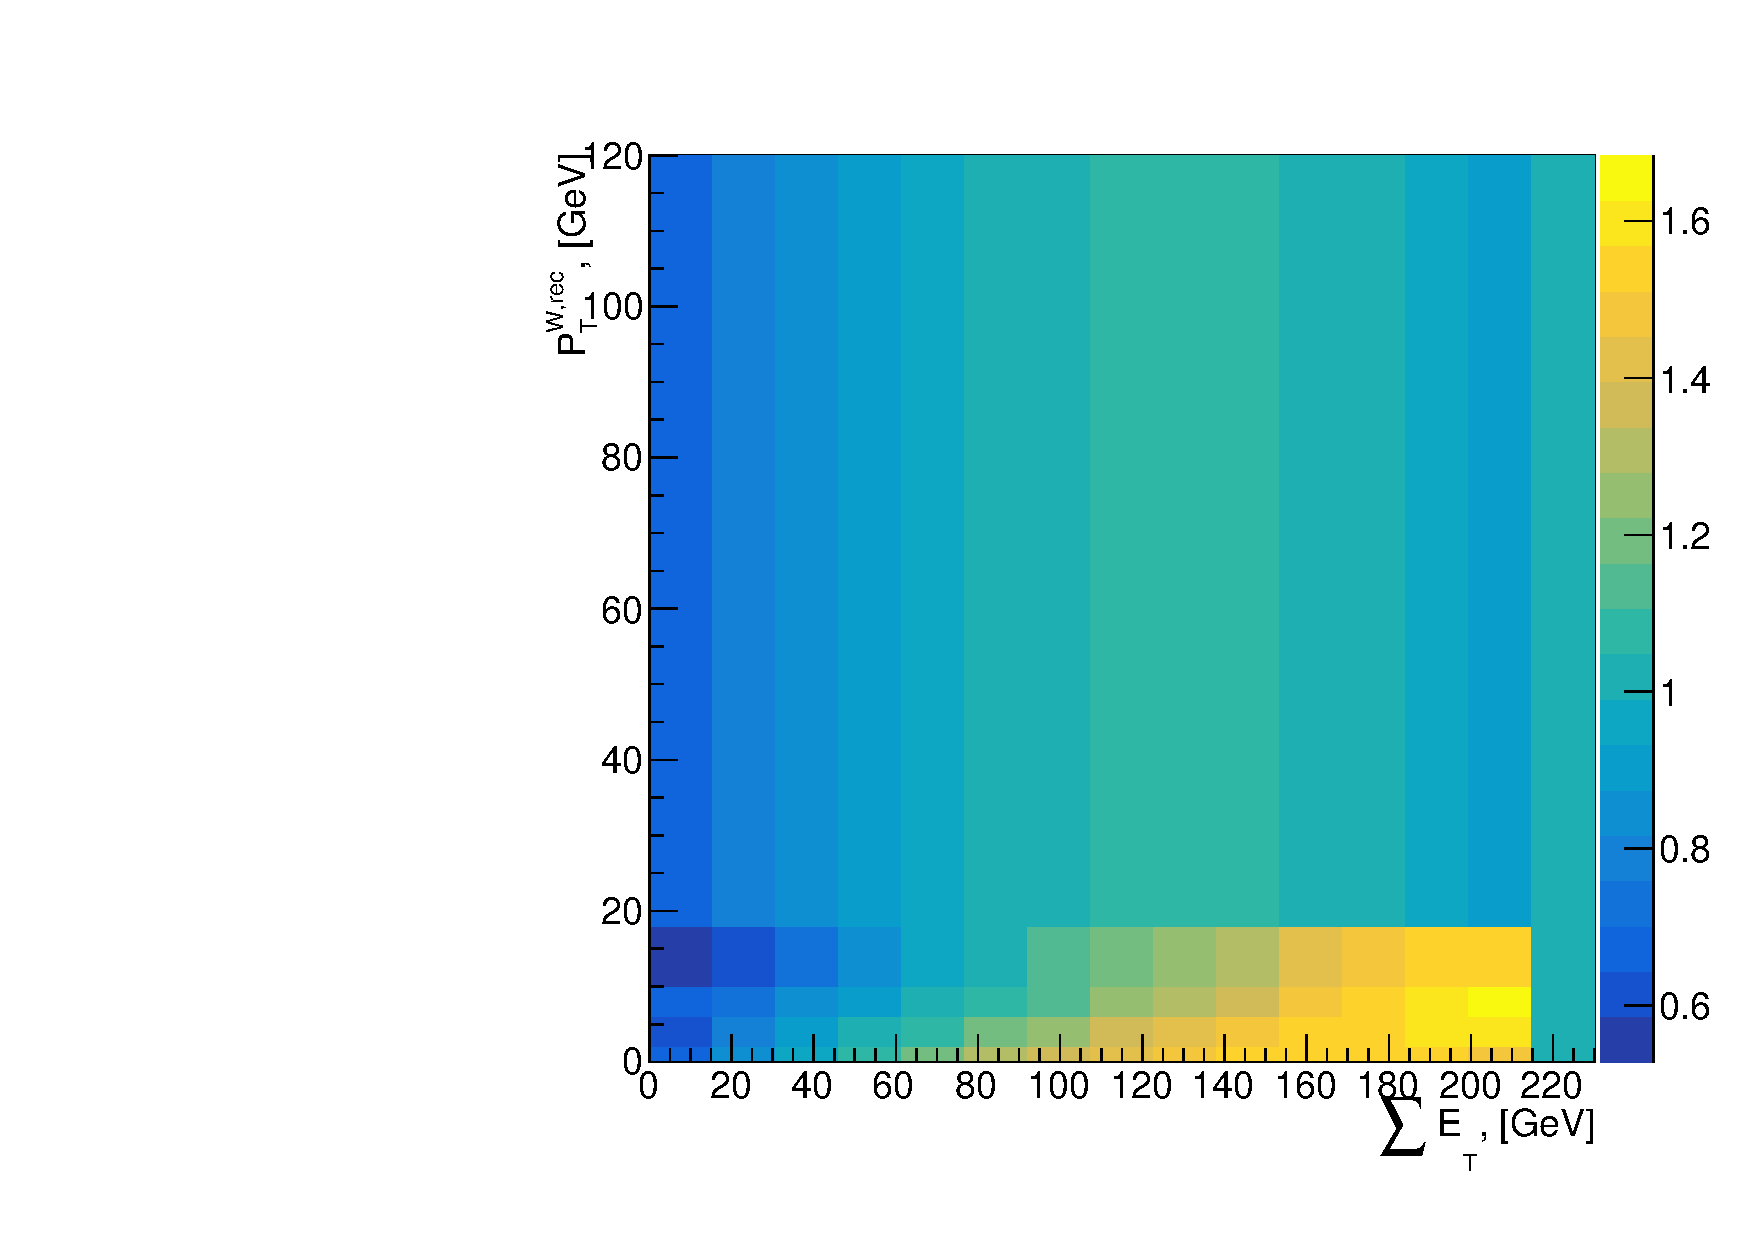
\includegraphics[width=1.\linewidth]{HadronRecoil/ReweightingPolEP.pdf} \\ a)}
\end{minipage}
\hfill
\begin{minipage}[h]{0.49\linewidth}
\center{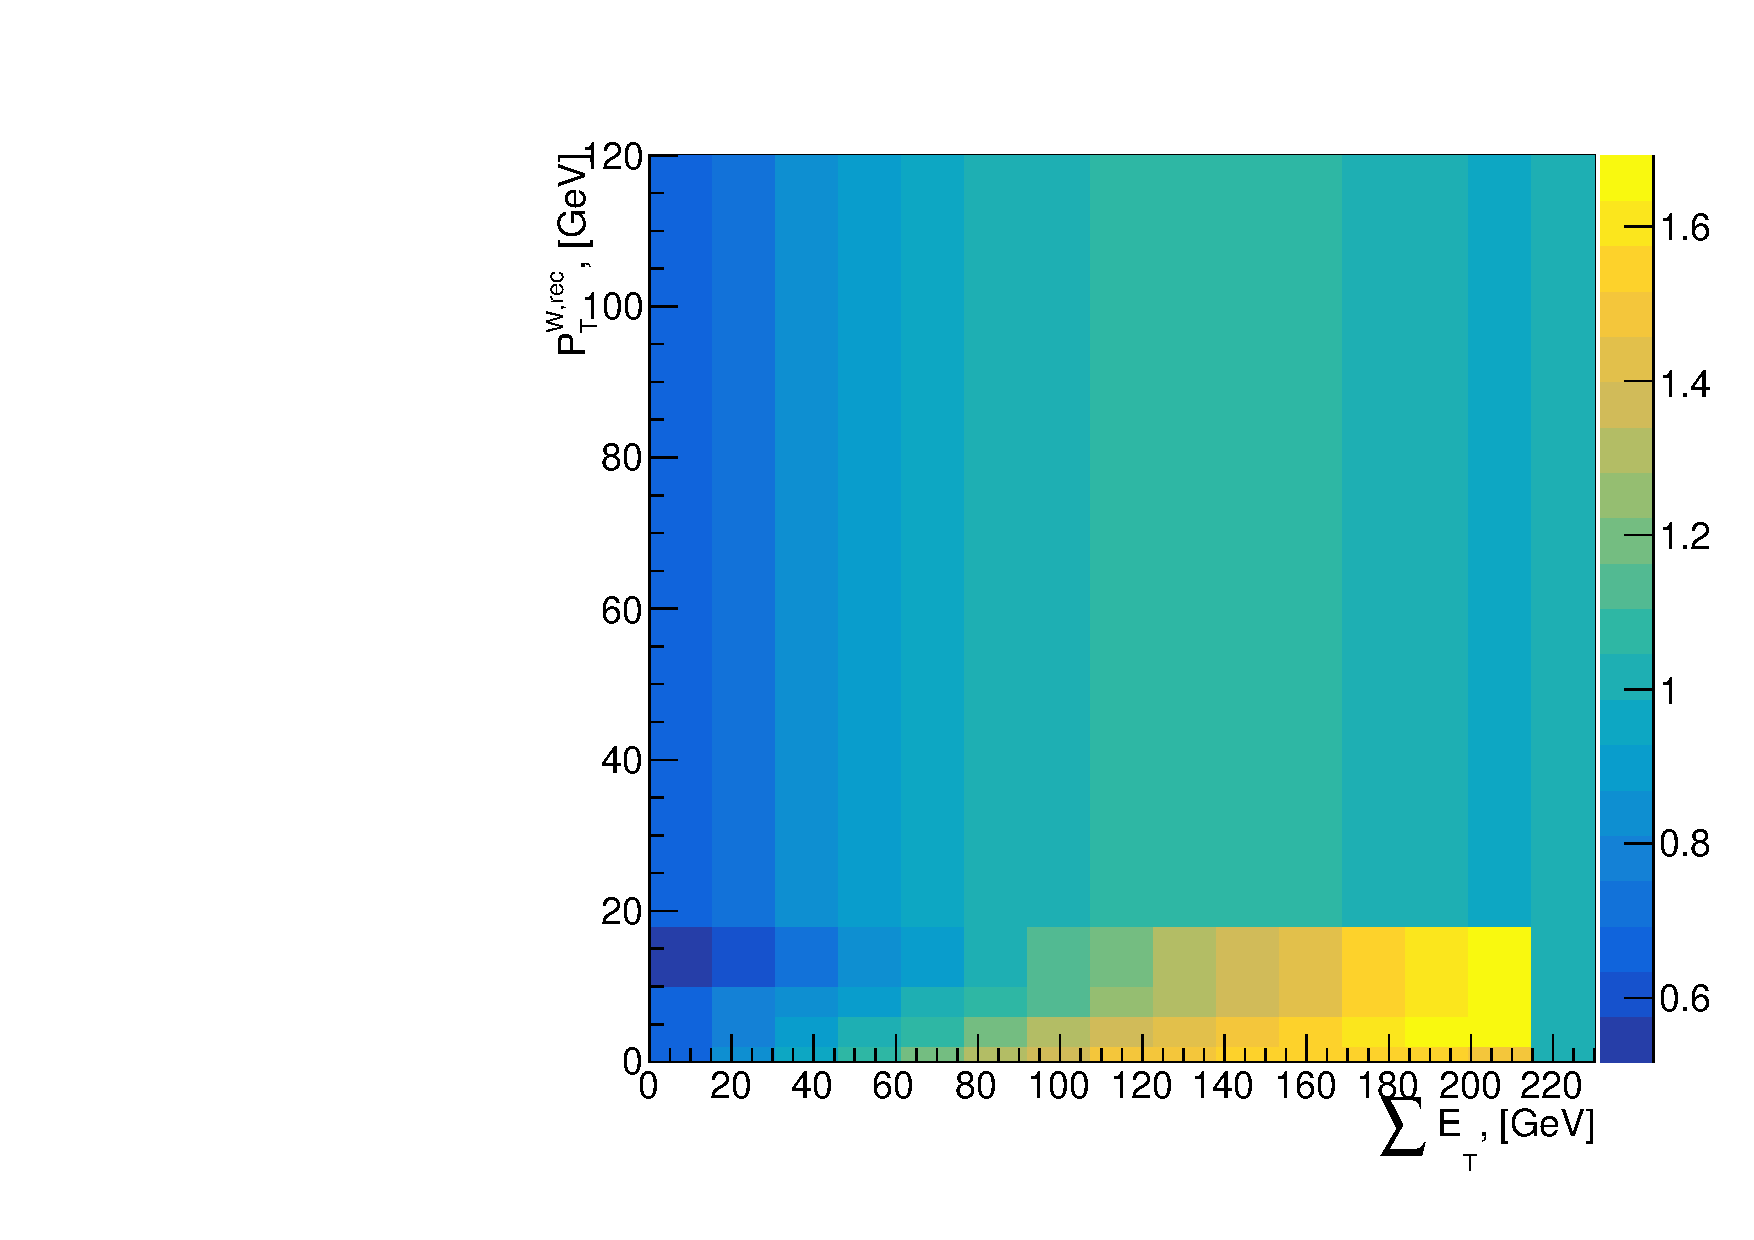
\includegraphics[width=1.\linewidth]{HadronRecoil/ReweightingPolMP.pdf} \\ b)}
\end{minipage}
\caption{Distribution of \sumet reweighting constants derived for a) $W^{+} \to e \nu$ and b) $W^{+} \to \mu \nu$ MC sample using polynomial order 2 approximation.}
\label{ris:SumEtCorPol}
\end{figure}

\subsubsection{Statistical error estimation}

Statistical error on the \sumet reweighting is estimated using Toy MC method, described in Chap.\ref{chap:Unc} from the polynomial order 2 approximation, since the uncertainty of the fit parameters obtained from the fit includes statistical error of data points. The fit parameters of the polynomials are varied inside each $p_T^{W, rec}$ bin within their fit uncertainties as in Eq. \ref{eq:ToyMethod}. 

Because of the possible correlations between the fit parameters, a multivariate gaussian distribution has been used. It  is calculated as:
\begin{equation}
p(x;\mu, \Sigma) =\frac{1}{(2\pi)^{n/2}|\Sigma|^{1/2}} exp\Big(-\frac{1}{2}(x-\mu)^{T}\Sigma^{-1}(x-\mu)\Big),
\end{equation}
where $\mu\in \boldsymbol{R}^{n}$ is obtained from the fit parameters vector and $\Sigma$ is $n \times n$ covariance matrix of these parameters, $(x-\mu)^{T}$ is a transpose of the vector $(x-\mu)$. In case of the polynomial order two n=3. For statistic error determination total number of 25 toys have been used. Total error is calculated using Eq.\ref{eq:ToyError}.

\subsubsection{Effect of the \sumet correction on cross-section}
The effect of the \sumet correction on cross-section is estimated by applying different correction factors on MC. The error is estimated by calculating difference in $C_{W}$ using On/Off method (see Chap. \ref{chap:Unc}). The overall effect of the \sumet correction for different methods is summarized in Tab. \ref{SumetCW}. Statistical error, estimated using Toy MC method is negligible. The systematic error is calculated as a difference between $C_{W}$ for a two methods and is considered to be small, compared to the overall effect. 

The sign of the effect differs for different W channels, that cannot be explained by a systematic error coming from the method or a data statistics. This effect also cannot be explained from a physical point of view, since we expect a similar errors for both lepton flavors, so it was decided not to use this corrections in a final analysis.

 \begin{table}[!t]
 \caption{Effect of \sumet correction on $C_{W}$ for different channels and methods}
\label{SumetCW}
\begin{center}
\begin{tabular}{c | c | c |  c |  c   }
\hline
Channel & $\delta C_W$ & $\delta C_W$ & $\delta C_W$ & $\delta C_W$ \\
& no approximation & polynomial order 2 & polynomial order 1 & Toy MC \\
\hline
\hline
$W^{+} \to e^{+}\nu$ & 0.48\% &0.39\%  & 0.31\% & 0.03\% \\
$W^{-} \to e^{-}\nu$ & 0.49\% &0.33\%  & 0.22\% & 0.03\% \\
$W^{+} \to \mu^{+}\nu$ & -0.27\% &-0.20\%  & -0.28\% & 0.03\% \\
$W^{-} \to \mu^{-}\nu$ & -0.29\% &-0.21\%  & -0.27\% & 0.03\% \\
\hline
\end{tabular}
\end{center}

\end{table}


\subsection{Resolution corrections using Z events}\label{sec:ZperpSmear}

Another way to check resolution effects is to study \uperp and \upar  $ - p_T^{Z}$ distributions in events containing Z boson. This correction assumes, that any resolution mismodelling reflects discrepancies in the \sumet distribution, while the difference in the resolution at a given \sumet is subleading. 

Difference in hadronic recoil resolutions $d\sigma$ between the data and the MC can be quantified by value:
\begin{equation}
d\sigma=\sqrt{\sigma_{data}^2-\sigma_{MC}^2},
\end{equation}
where $\sigma_{data}$ and $\sigma_{MC}$ are the RMS of these distributions. This value is affected by the statistical uncertainty of data standard deviation, that in case of the distributions close to normal can be calculated as \cite{AdvStat}:
\begin{equation}
\sigma( \sigma_{data} ) = \frac{\sigma_{data}}{\sqrt{2N} },
\end{equation}
where $N$ is the number of entries in histogram. The distributions of \uperp and \upar  $ - p_T^{Z}$ in $Z\to ee$, $Z\to \mu\mu$, $Z\to ll$ events are shown in Fig. \ref{HadrRecoil:UparSmear}. The typical resolution uncertainty for data is around 0.1 GeV for all distributions, while the the difference in resolution is 1.0 GeV and higher, that is a clear indication of mismodelling of hadronic recoil resolution in the Monte-Carlo. The overall difference in resolutions is consistent between \uperp and \upar  $ - p_T^{Z}$ distributions, however it depends on a lepton flavor, isolation and identification criteria. For a correction it was decided to choose the value, obtained from combined $Z\to ll$ channel, where $d\sigma$ = 1.3 GeV.

\begin{figure}[!tbp]
\begin{minipage}[h]{0.32\linewidth}
\center{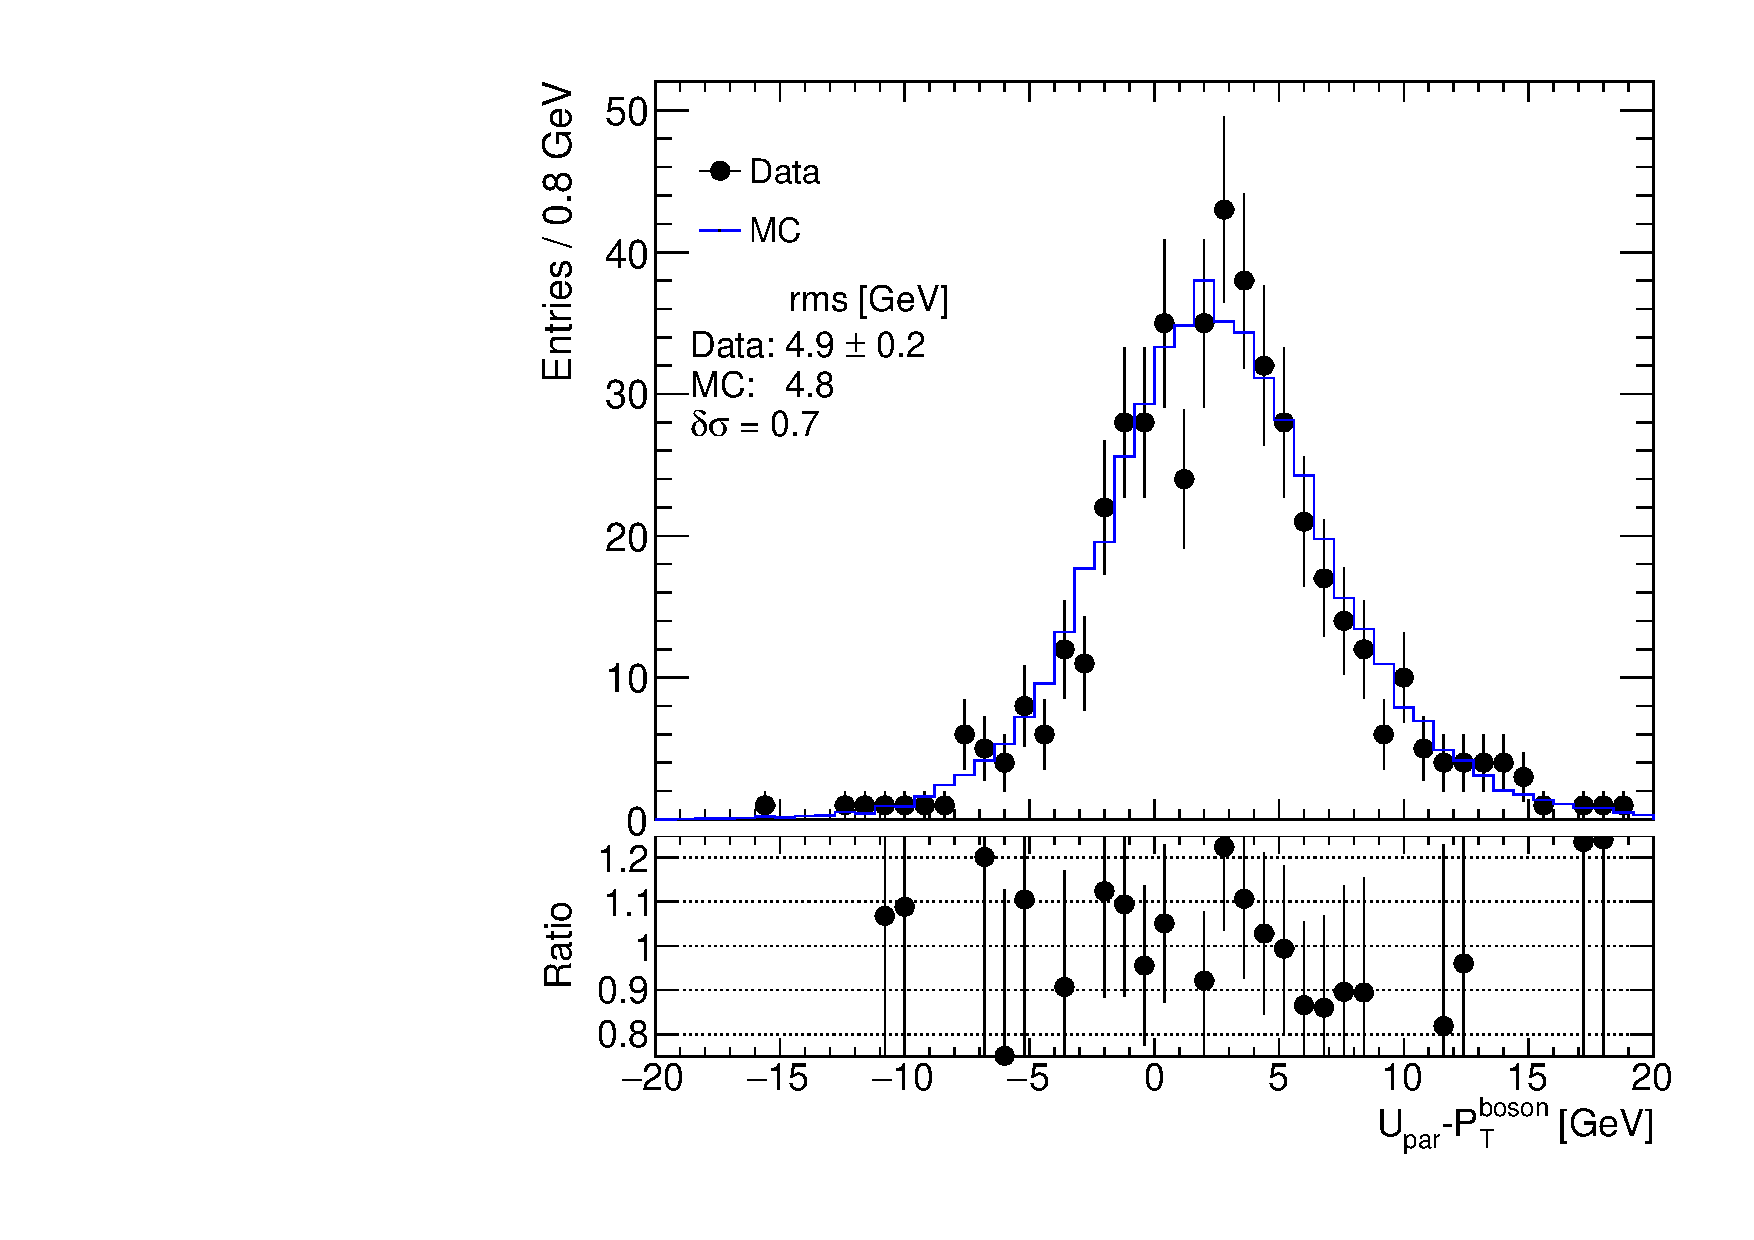
\includegraphics[width=1.\linewidth]{HadronRecoil/UParERMS.pdf} \\ a)}
\end{minipage}
\hfill
\begin{minipage}[h]{0.32\linewidth}
\center{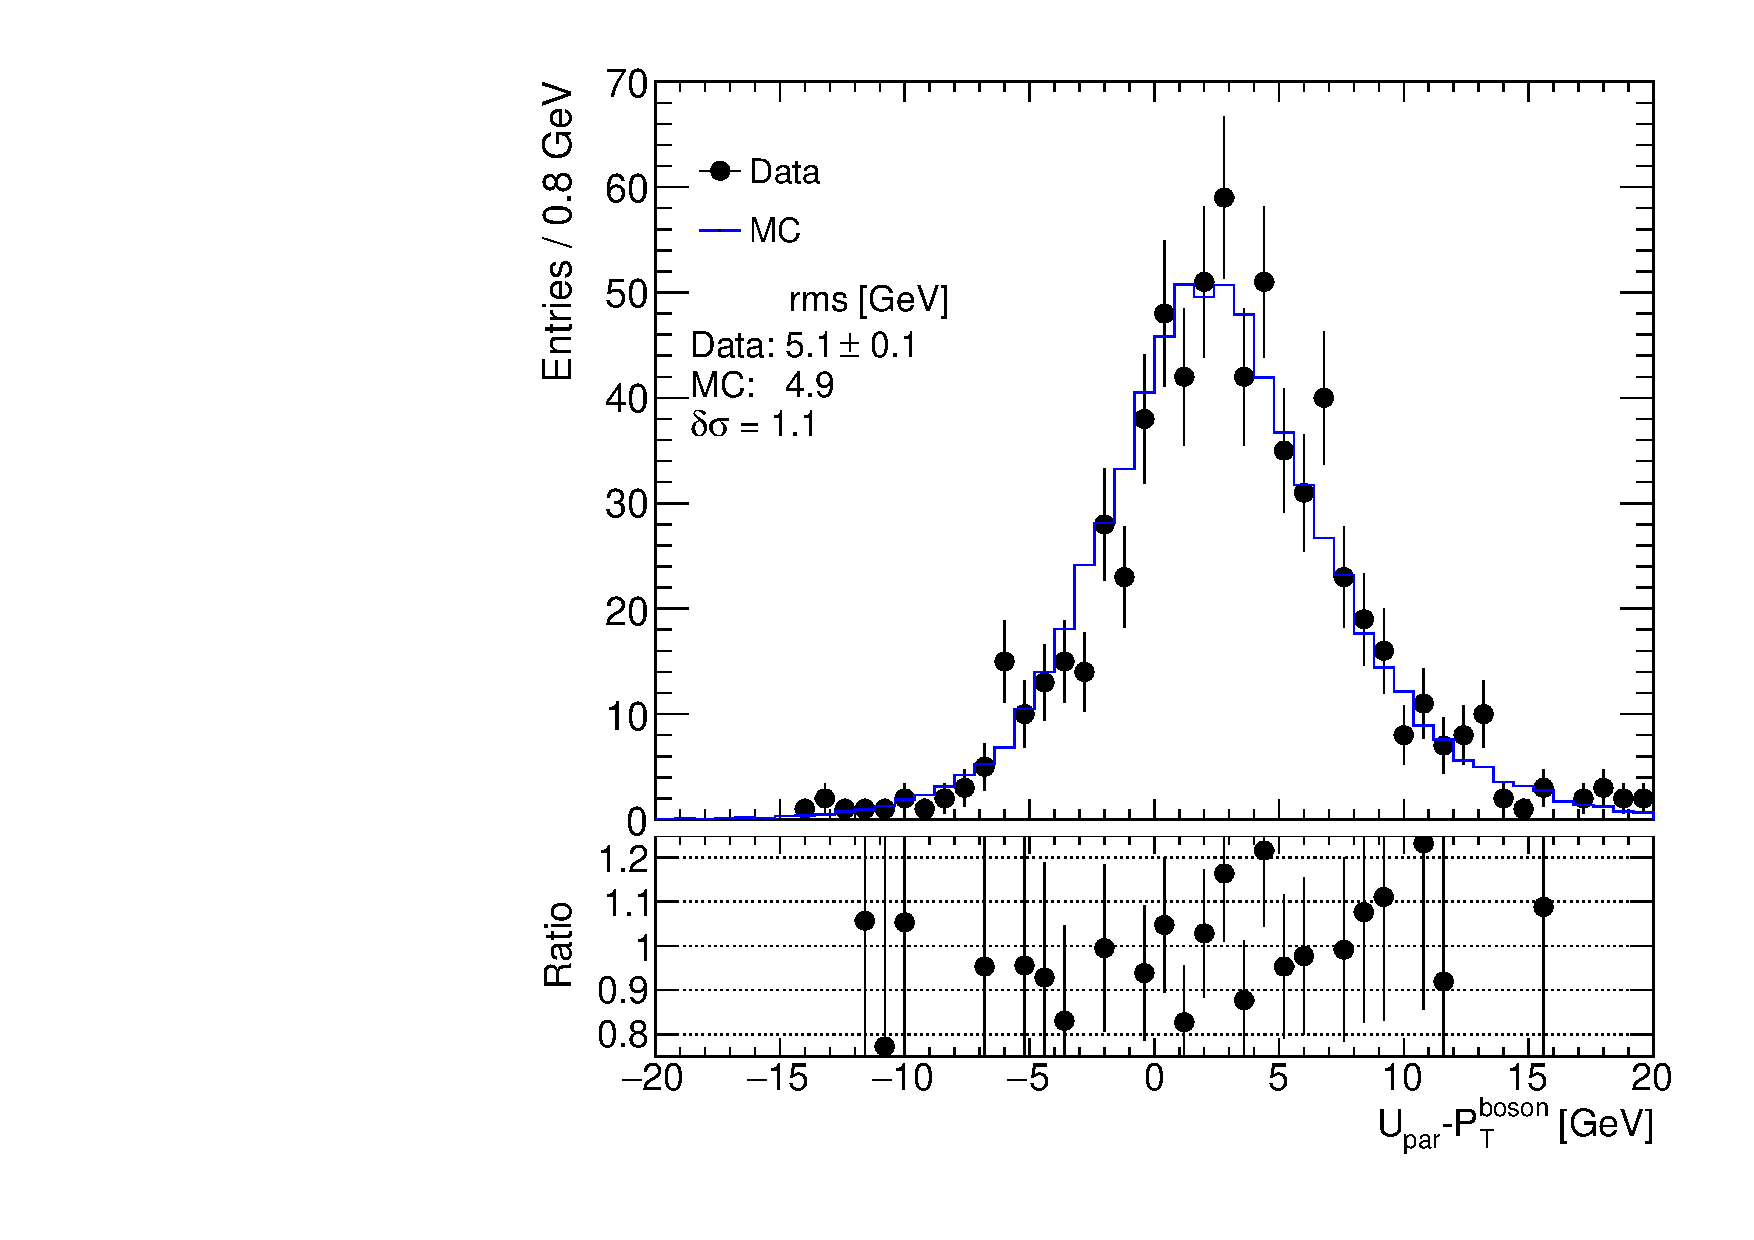
\includegraphics[width=1.\linewidth]{HadronRecoil/UParMRMS.pdf} \\ b)}
\end{minipage}
\hfill
\begin{minipage}[h]{0.32\linewidth}
\center{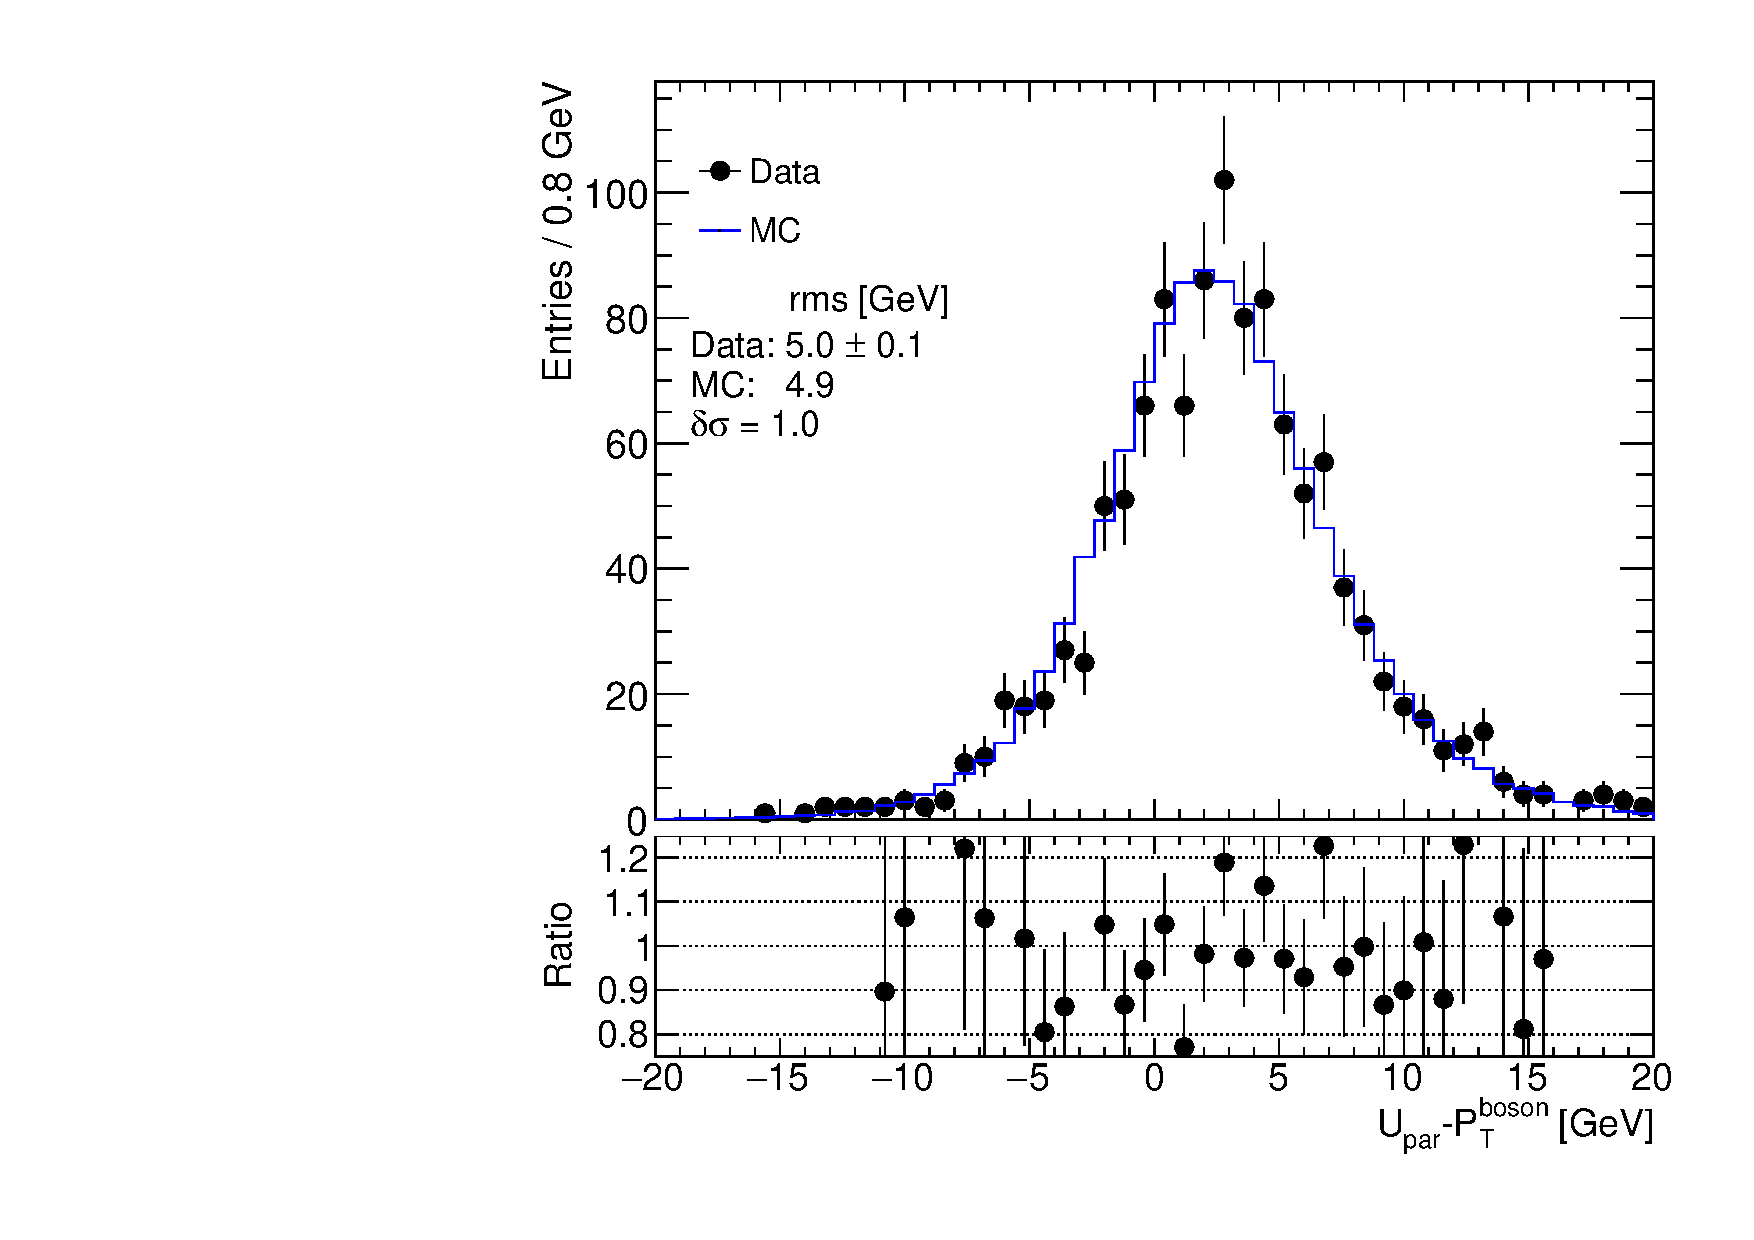
\includegraphics[width=1.\linewidth]{HadronRecoil/UParTotalRMS.pdf} \\ c)}
\end{minipage}
\caption{Parallel hadronic recoil component distribuiton from a) the $Z\to ee$ selection b) $Z\to\mu\mu$ selection and c) $Z\to ll$ selection. The expected contribution from signal is estimated with Monte Carlo simulation, other background sources are considered negligible.}
\label{HadrRecoil:UparSmear}
\end{figure}

\begin{figure}[!tbp]
\begin{minipage}[h]{0.32\linewidth}
\center{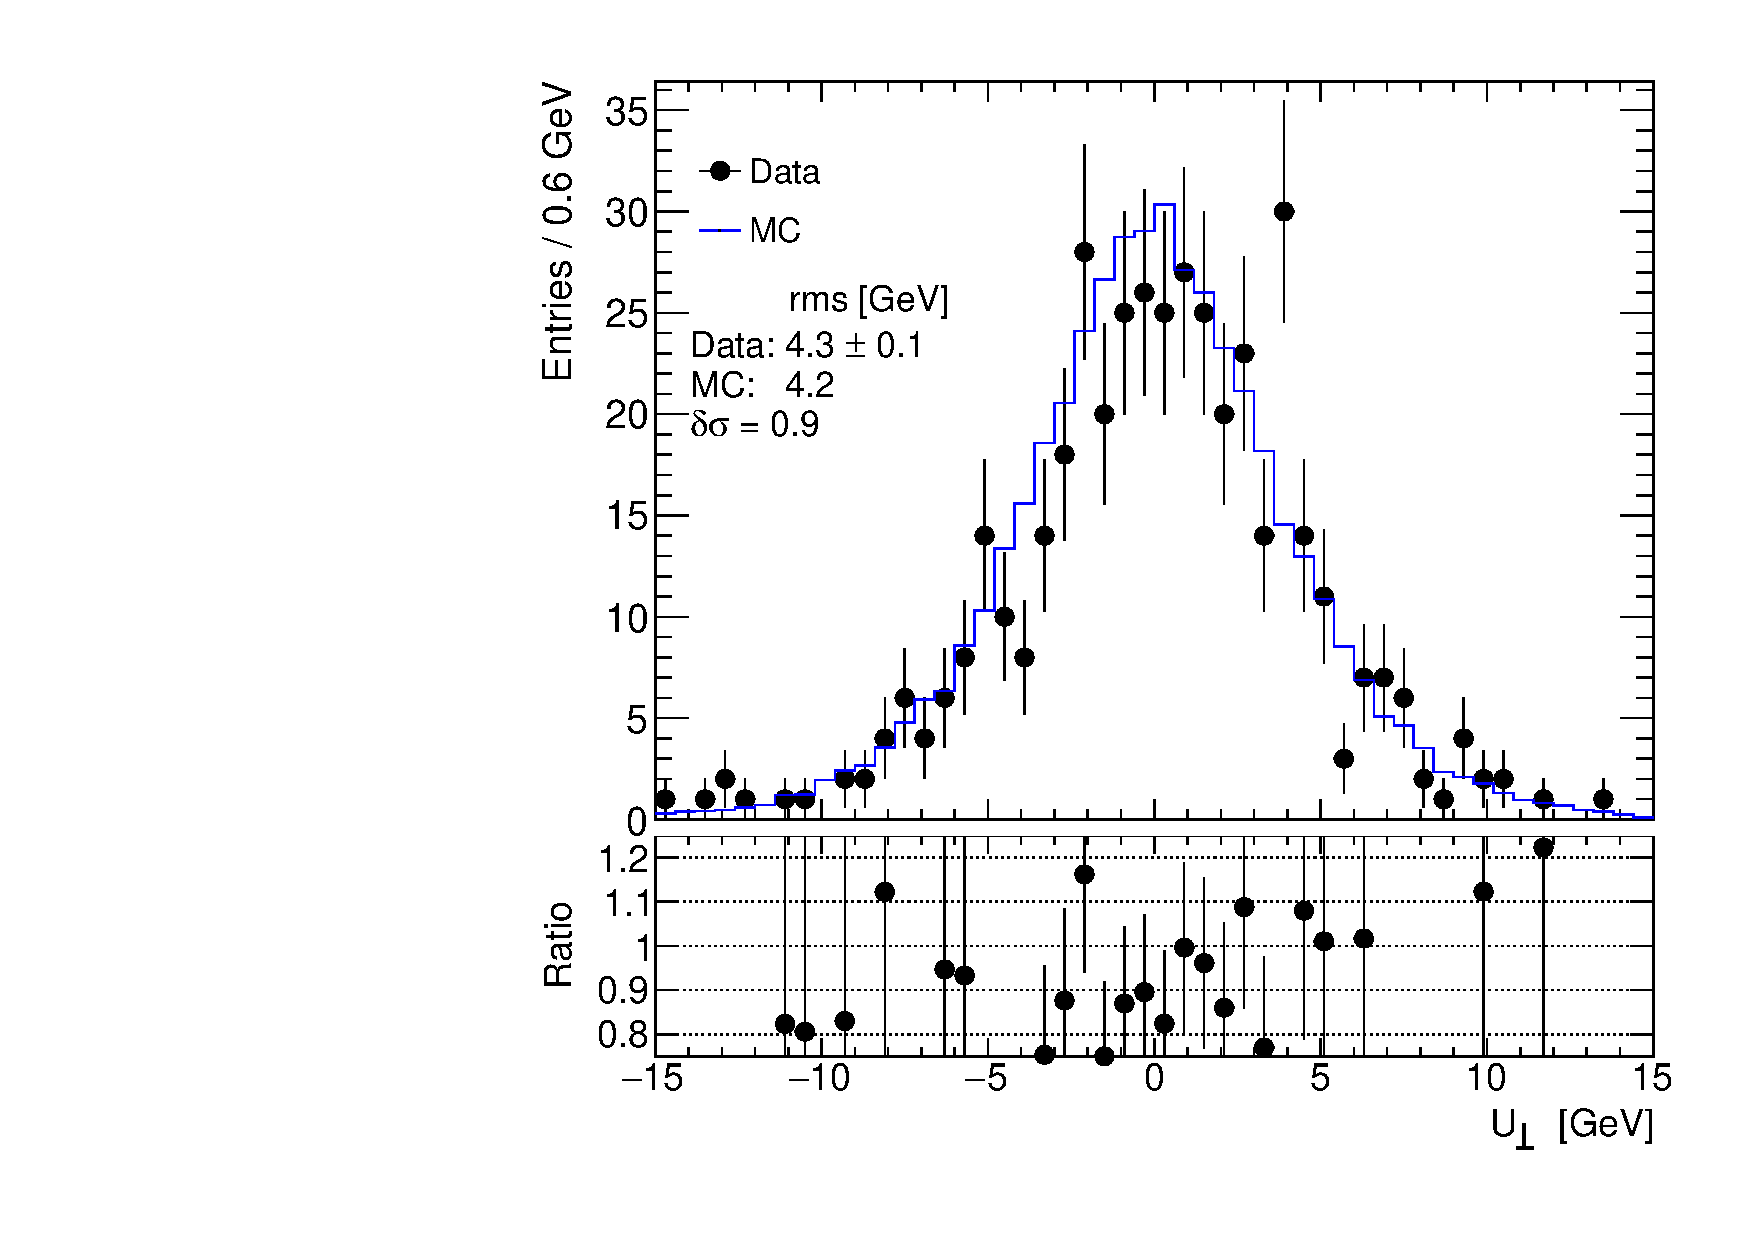
\includegraphics[width=1.\linewidth]{HadronRecoil/UPerpERMS.pdf} \\ a)}
\end{minipage}
\hfill
\begin{minipage}[h]{0.32\linewidth}
\center{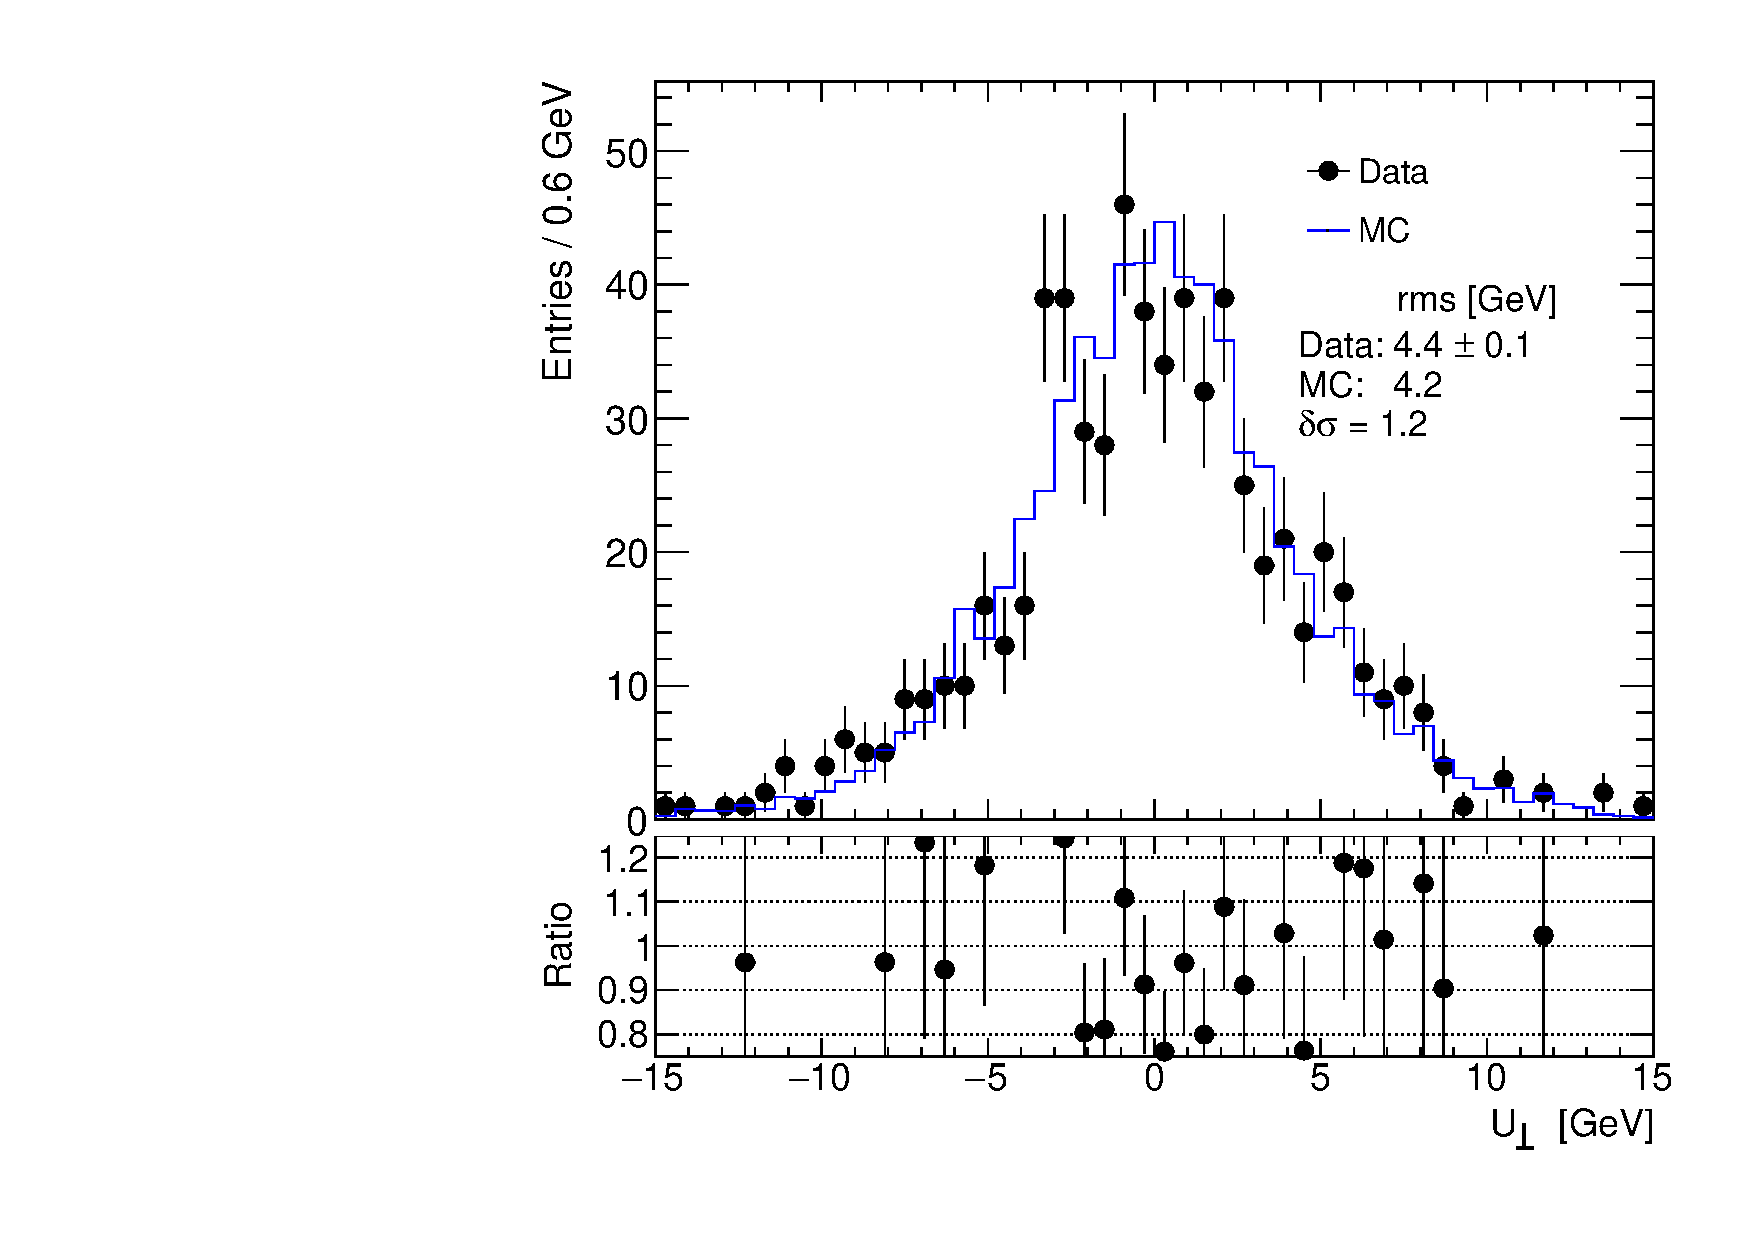
\includegraphics[width=1.\linewidth]{HadronRecoil/UPerpMRMS.pdf} \\ b)}
\end{minipage}
\hfill
\begin{minipage}[h]{0.32\linewidth}
\center{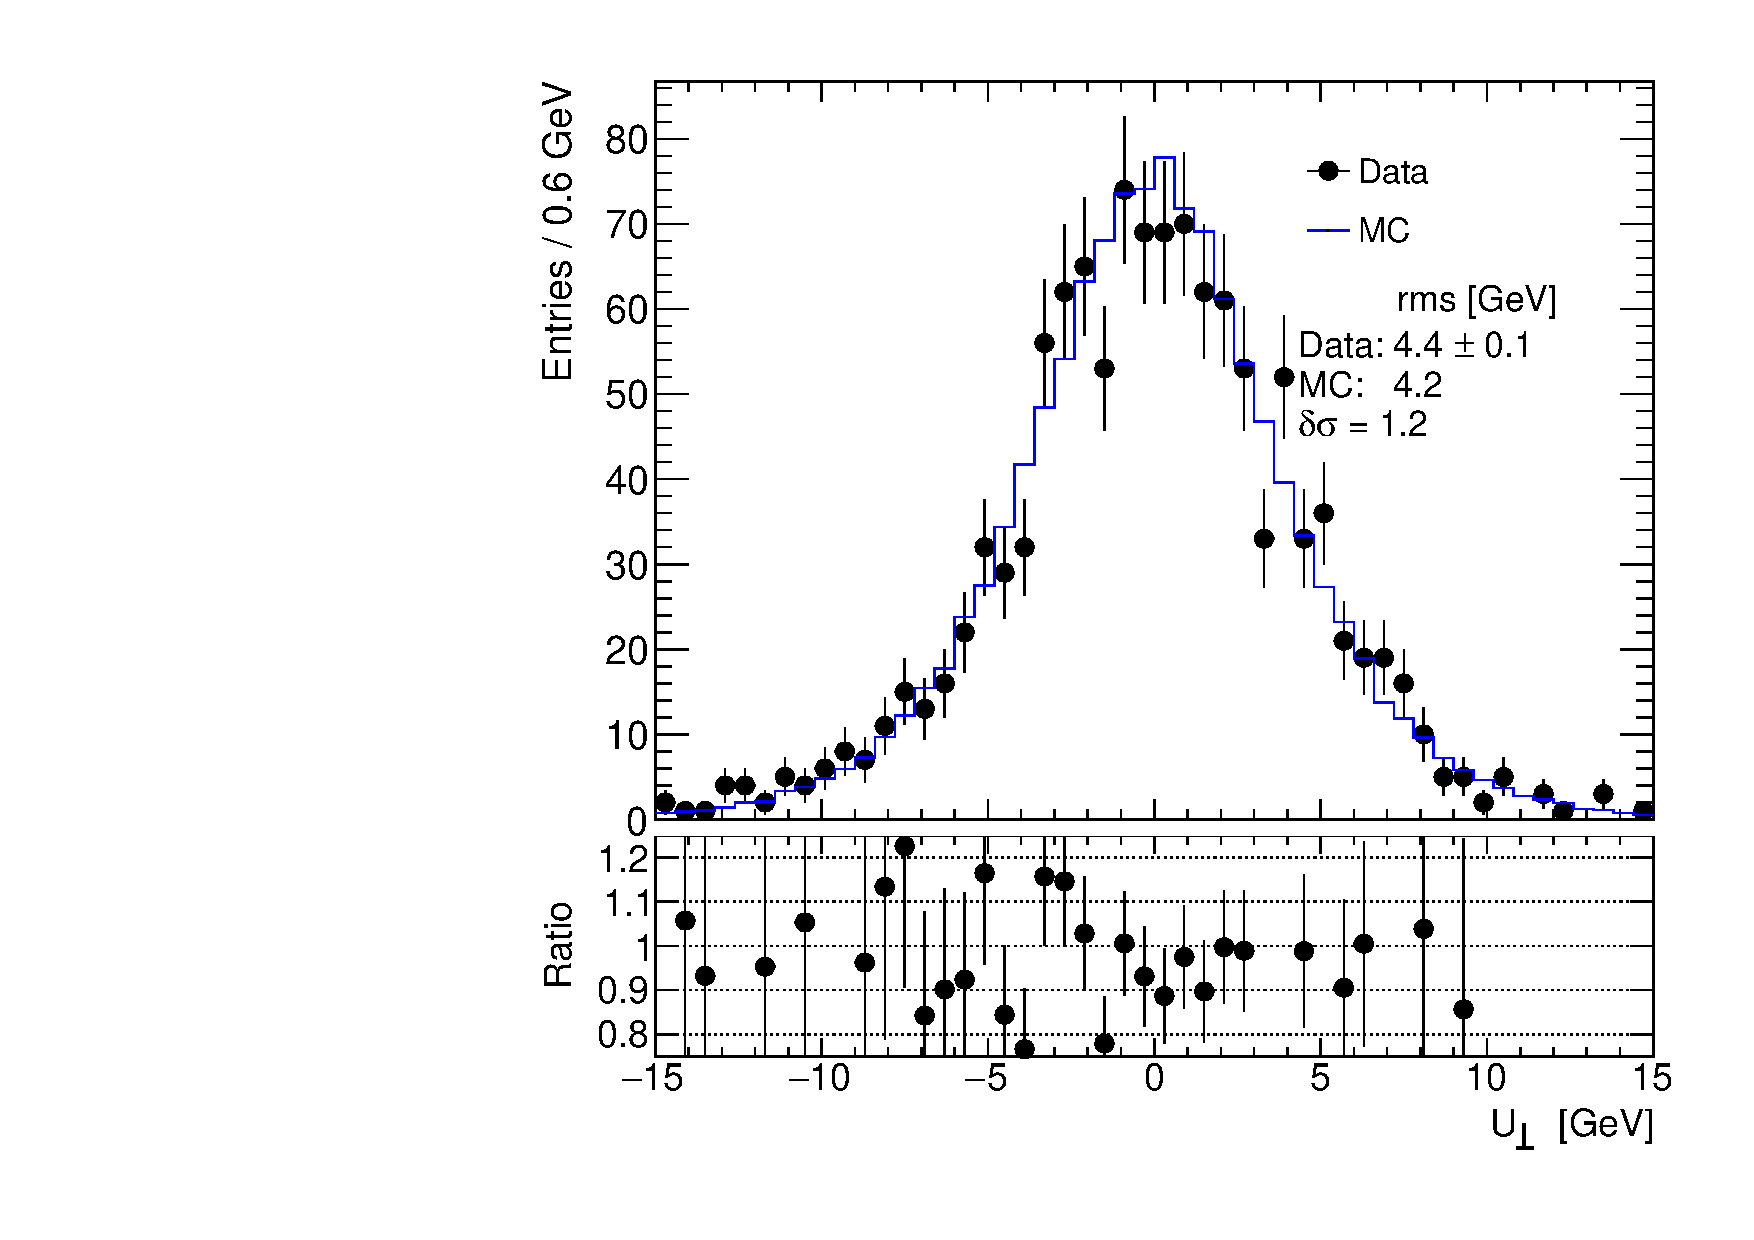
\includegraphics[width=1.\linewidth]{HadronRecoil/UPerpTotalRMS.pdf} \\ c)}
\end{minipage}
\caption{Perpendicular hadronic recoil component distribuiton from a) the $Z\to ee$ selection b) $Z\to\mu\mu$ selection and c) $Z\to ll$ selection. The expected contribution from signal is estimated with Monte Carlo simulation, other background sources are considered negligible.}
\label{HadrRecoil:UpeprSmear}
\end{figure}

The resolution is corrected by a smearing, using a Gaussian distribution, of each component of the hadronic recoil in Monte-Carlo:
\begin{equation}
\upar' = \upar+Gaus(0, d\sigma)
\end{equation}
\begin{equation}
\uperp' = \uperp + Gaus(0, d\sigma),
\end{equation}

\subsubsection{Effect of the smearing correction on cross-section}

\begin{figure}[!tbp]
\begin{minipage}[h]{0.49\linewidth}
\center{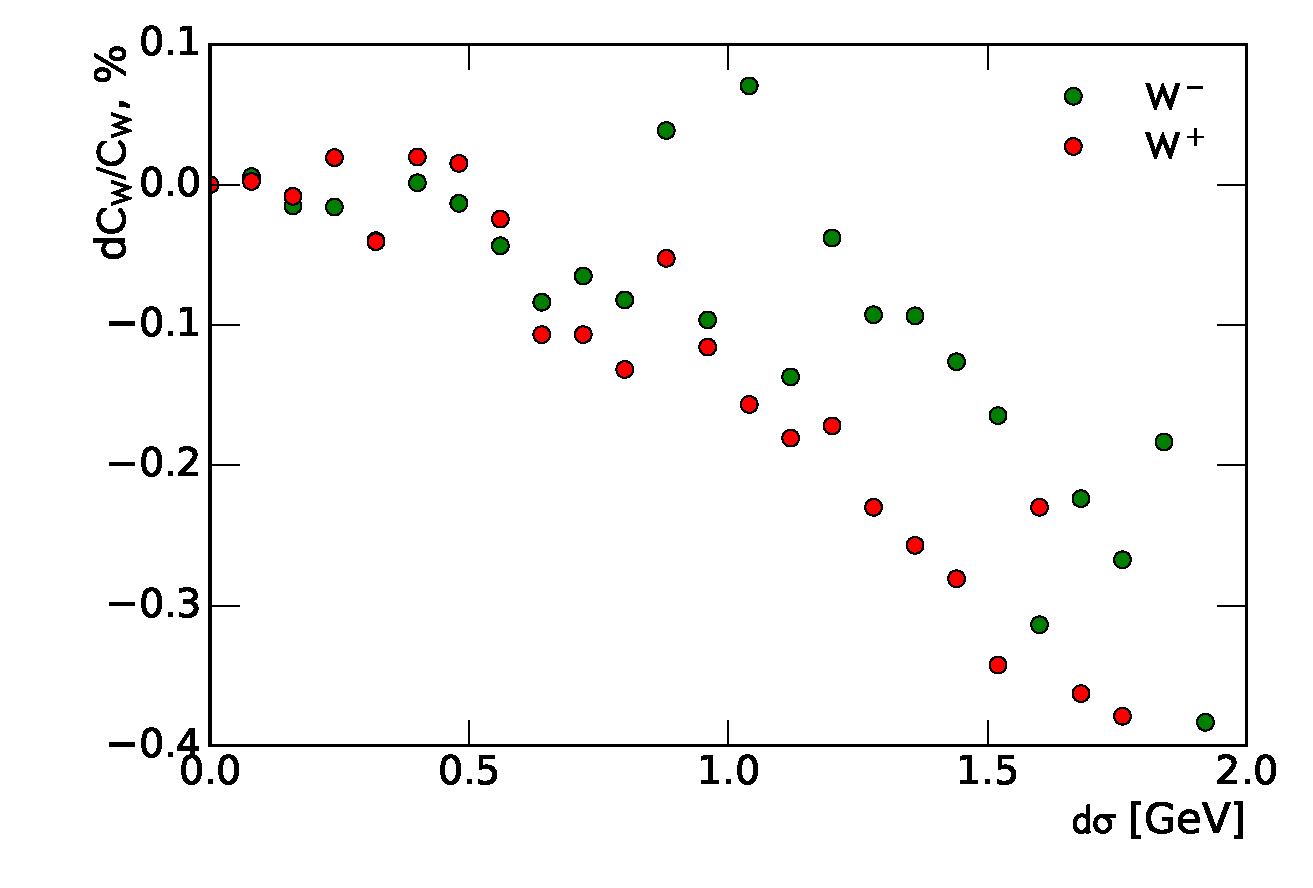
\includegraphics[width=1.\linewidth]{HadronRecoil/CWElectronSmearing.pdf} \\ a)}
\end{minipage}
\hfill
\begin{minipage}[h]{0.49\linewidth}
\center{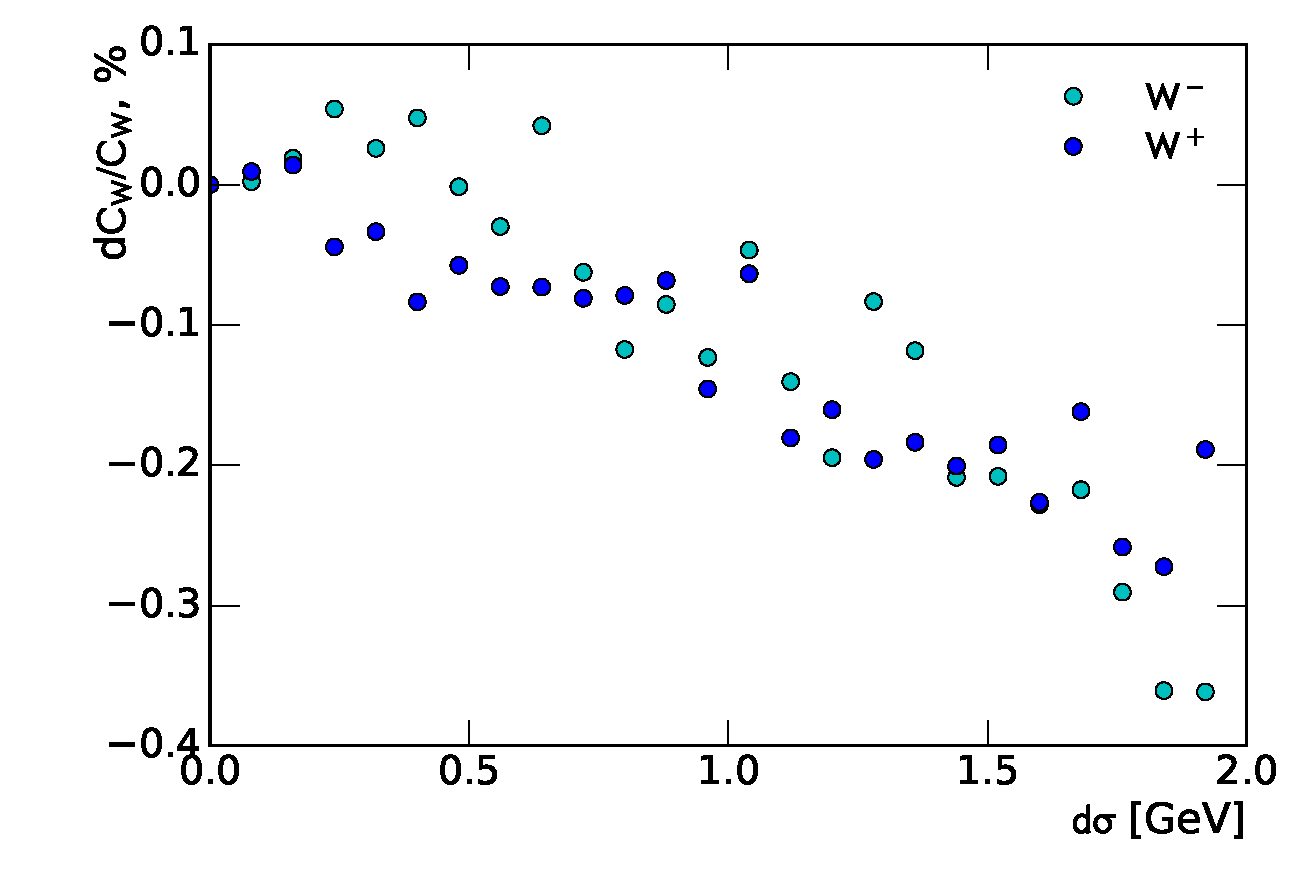
\includegraphics[width=1.\linewidth]{HadronRecoil/CWMuonSmearing.pdf} \\ b)}
\end{minipage}
\caption{Effect on a \cw from hadronic recoil resolution correction with different $d\sigma$ for a) \wenu b) \wmunu channel.}
\label{ris:HadrRecSmearScan}
\end{figure}

\begin{figure}[!tbp]
\begin{minipage}[h]{0.49\linewidth}
\center{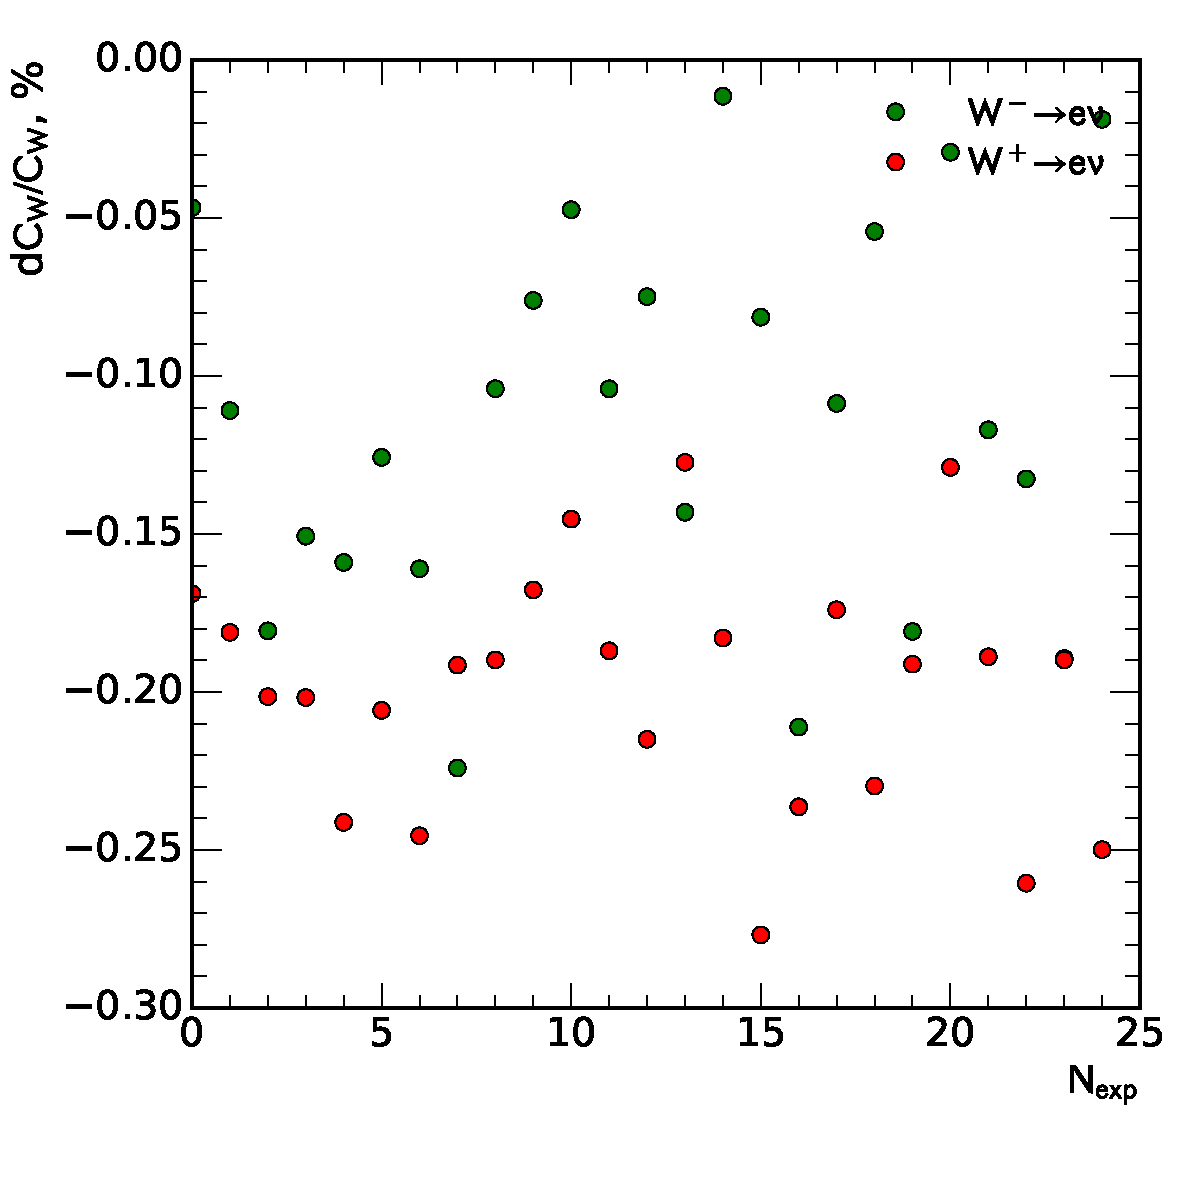
\includegraphics[width=1.\linewidth]{HadronRecoil/CWElectronStab.pdf} \\ a)}
\end{minipage}
\hfill
\begin{minipage}[h]{0.49\linewidth}
\center{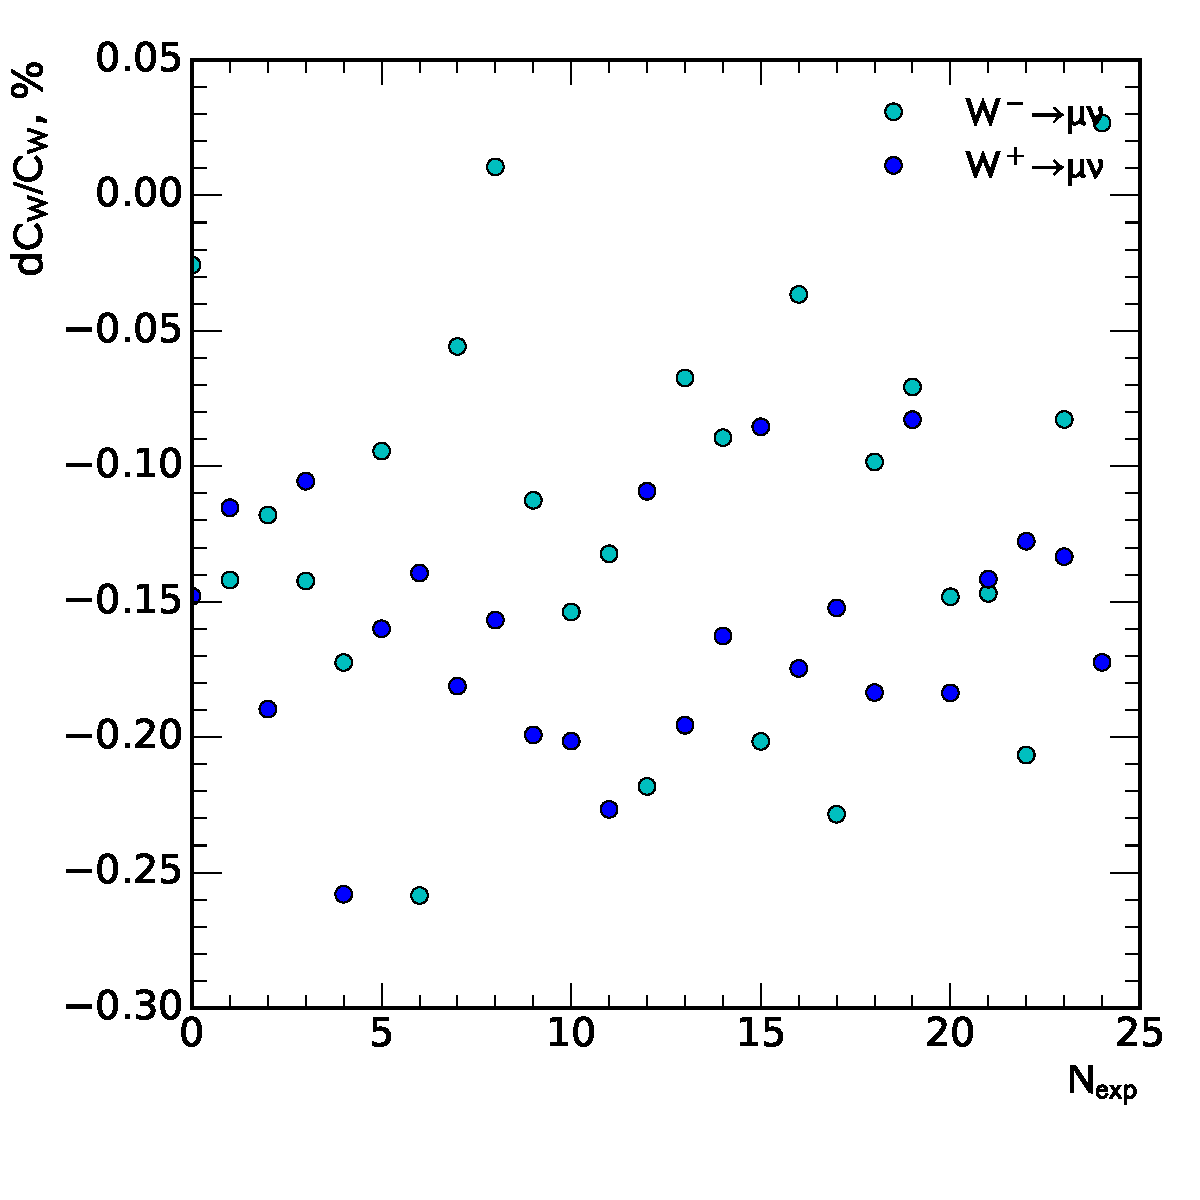
\includegraphics[width=1.\linewidth]{HadronRecoil/CWMuonStab.pdf} \\ b)}
\end{minipage}
\caption{Effect on a \cw from hadronic recoil resolution correction with $d\sigma$ = 1.3 GeV for a) \wenu b) \wmunu channel for repeated experiments. The overall systematic uncertainty of this correction is estimated as the mean value of $dC_{W}$. }
\label{ris:HadrRecSmearStab}
\end{figure}

Effect of smearing correction is estimated using On/Off method (Chap. \ref{chap:Unc}) on a $C_{W}$ factor. Scan in a big range of the  parameter $d\sigma$ up to  2.0 GeV (Fig. \ref{ris:HadrRecSmearScan}) have showed, that $C_{W}$ becomes smaller with growth of the smearing parameter $d\sigma$. However, due to the random nature of the correction, the $C_{W}$ fluctuates within the mean value.

Systematic error have been estimated by repeating correction on the same sample 25 times (Fig. \ref{ris:HadrRecSmearStab}). Table \ref{SmearCW} presents the mean effect on $C_{W}$ together with the rms of the distribution. Overall systematic effect is below 0.2\% for each analysis channel, that makes it negligible compared to the statistics uncertainty in W samples (Chap. \ref{chap:Unc}).


 \begin{table}[!t]
 \caption{Effect of smearing correction on a $C_{W}$ for a different channels. The statistical error (noted $stat.err.$) of the mean value is estimated using the Eq. \ref{eq:MeanErr}}
\label{SmearCW}
\begin{center}
\begin{tabular}{| l  | c | c | }
\hline
Channel & $\delta C_W \pm stat.err.$ & rms \\
\hline
\hline
$W^{+} \to e^{+}\nu$ & -0.20$\pm0.01$\% & 0.04\% \\
$W^{-} \to e^{-}\nu$ & -0.11$\pm0.01$\% &  0.06\% \\
\hline
$W^{+} \to \mu^{+}\nu$ & -0.16$\pm0.01$\% & 0.04\% \\
$W^{-} \to \mu^{-}\nu$ & -0.12$\pm0.01$\% & 0.07\% \\
\hline
\end{tabular}
\end{center}

\end{table}

\section{Hadronic recoil bias correction}

\begin{figure}[!b]
\minipage{0.32\textwidth}
  \center{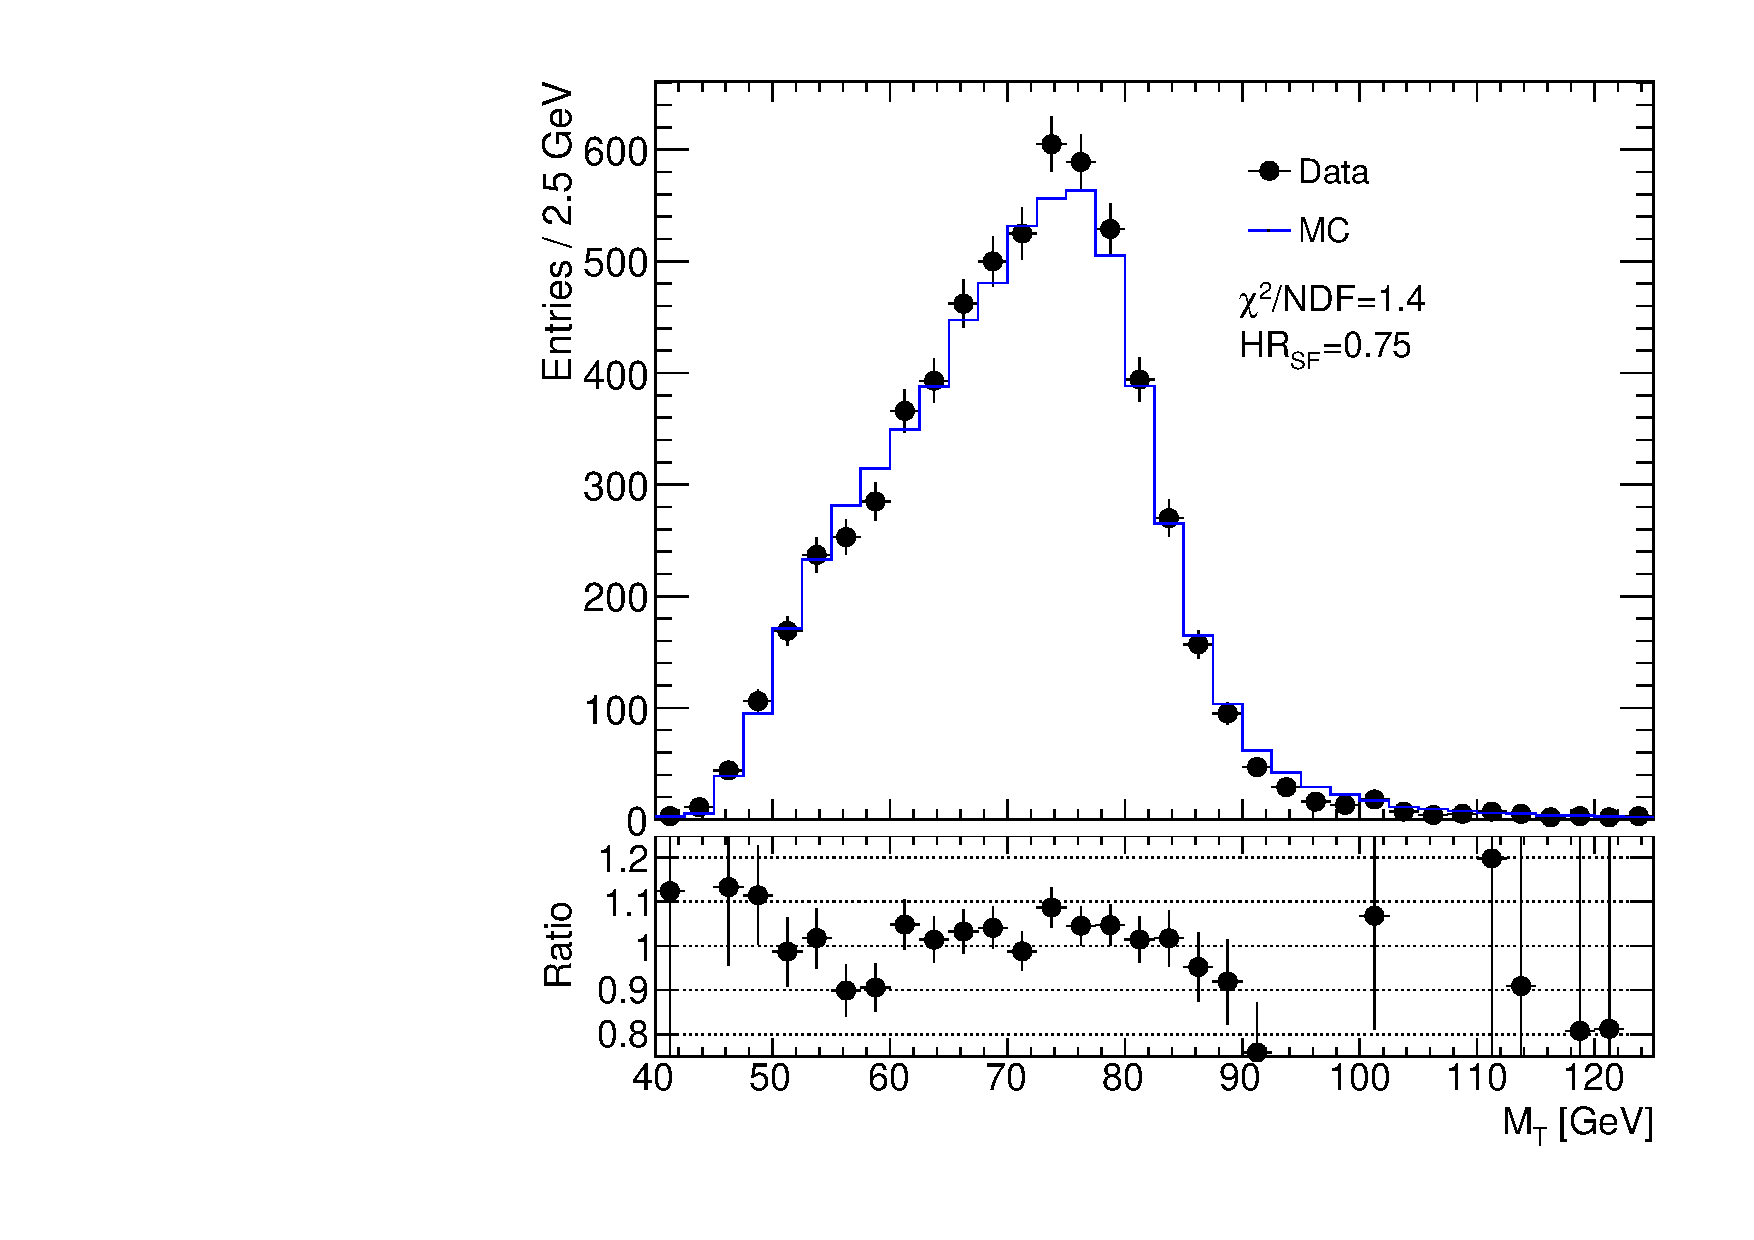
\includegraphics[width=\linewidth]{HadronRecoil/MtWEScale0.pdf} a)}
\endminipage\hfill
\minipage{0.32\textwidth}
   \center{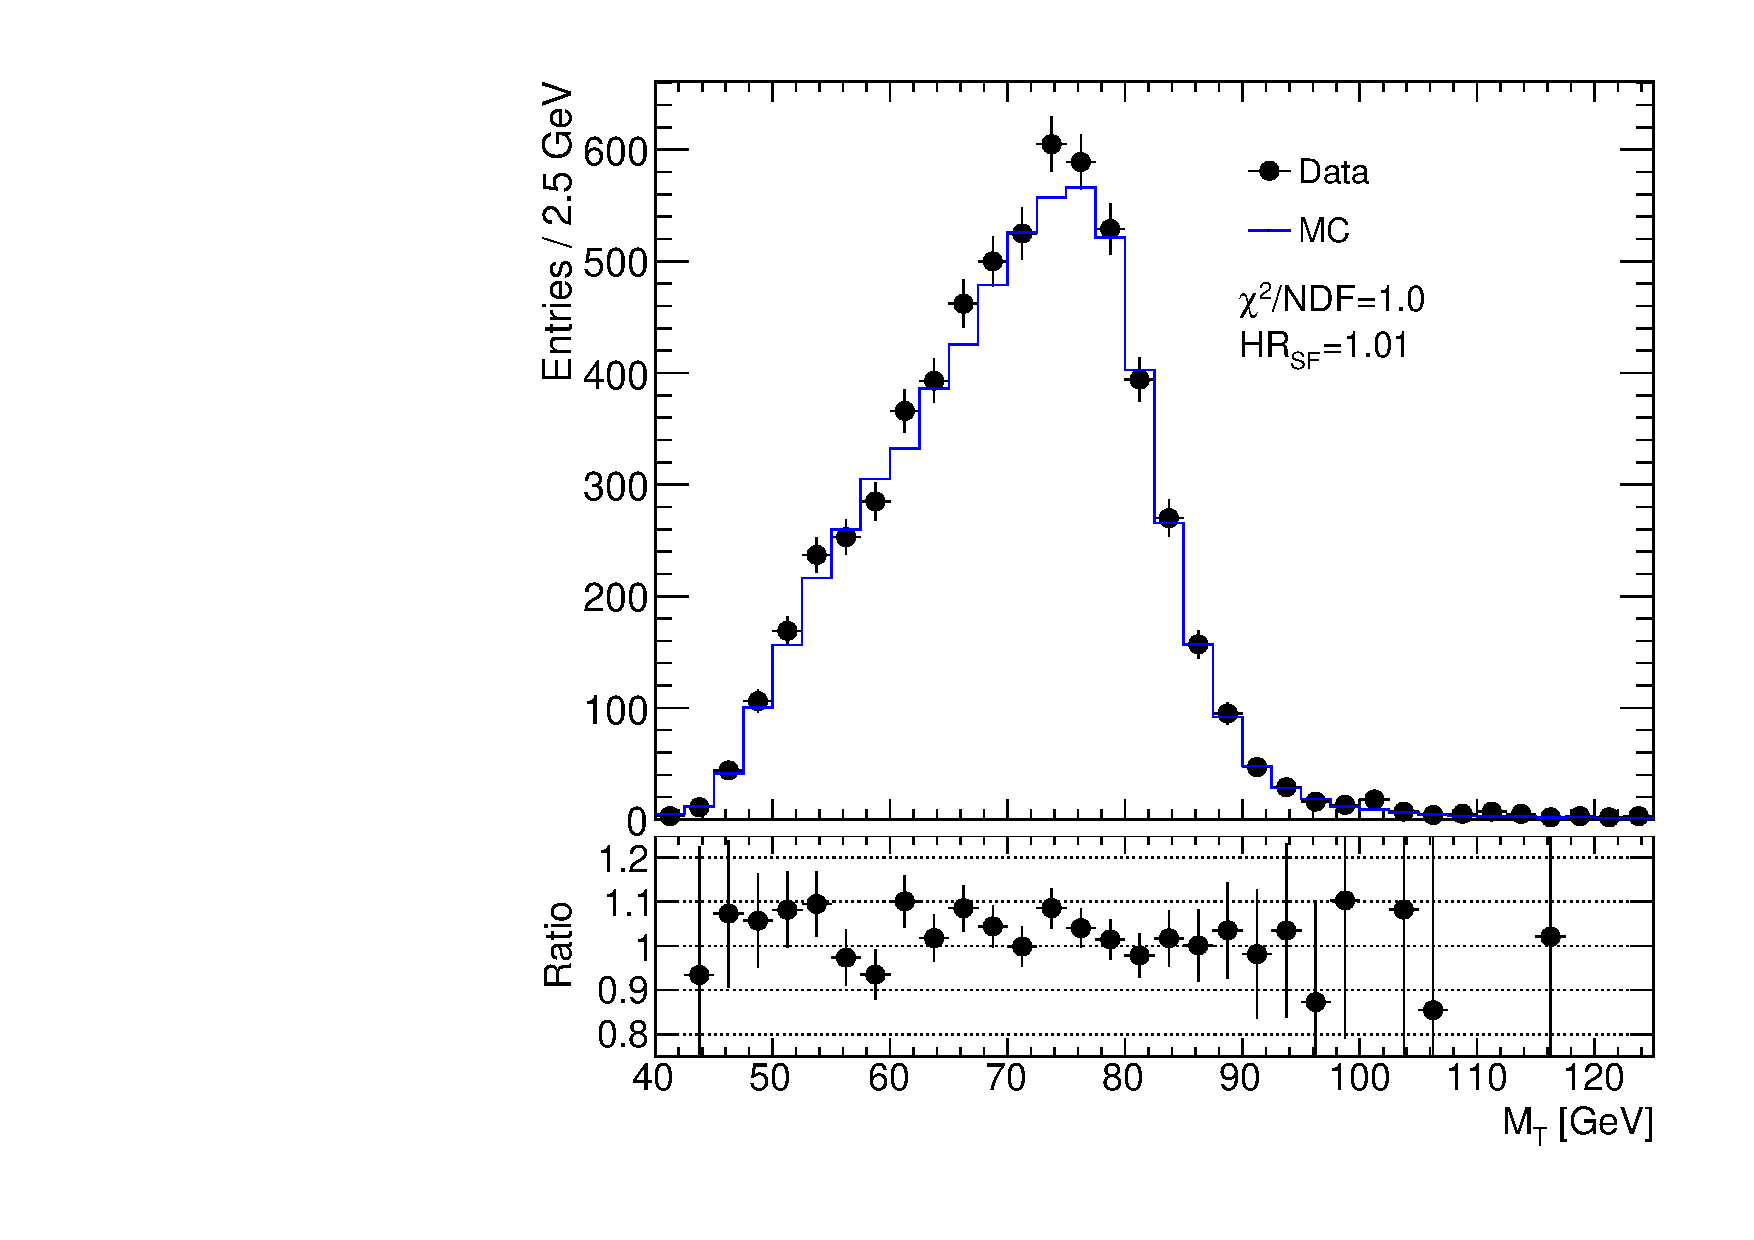
\includegraphics[width=\linewidth]{HadronRecoil/MtWEScale13.pdf} b)}
\endminipage\hfill
\minipage{0.32\textwidth}%
   \center{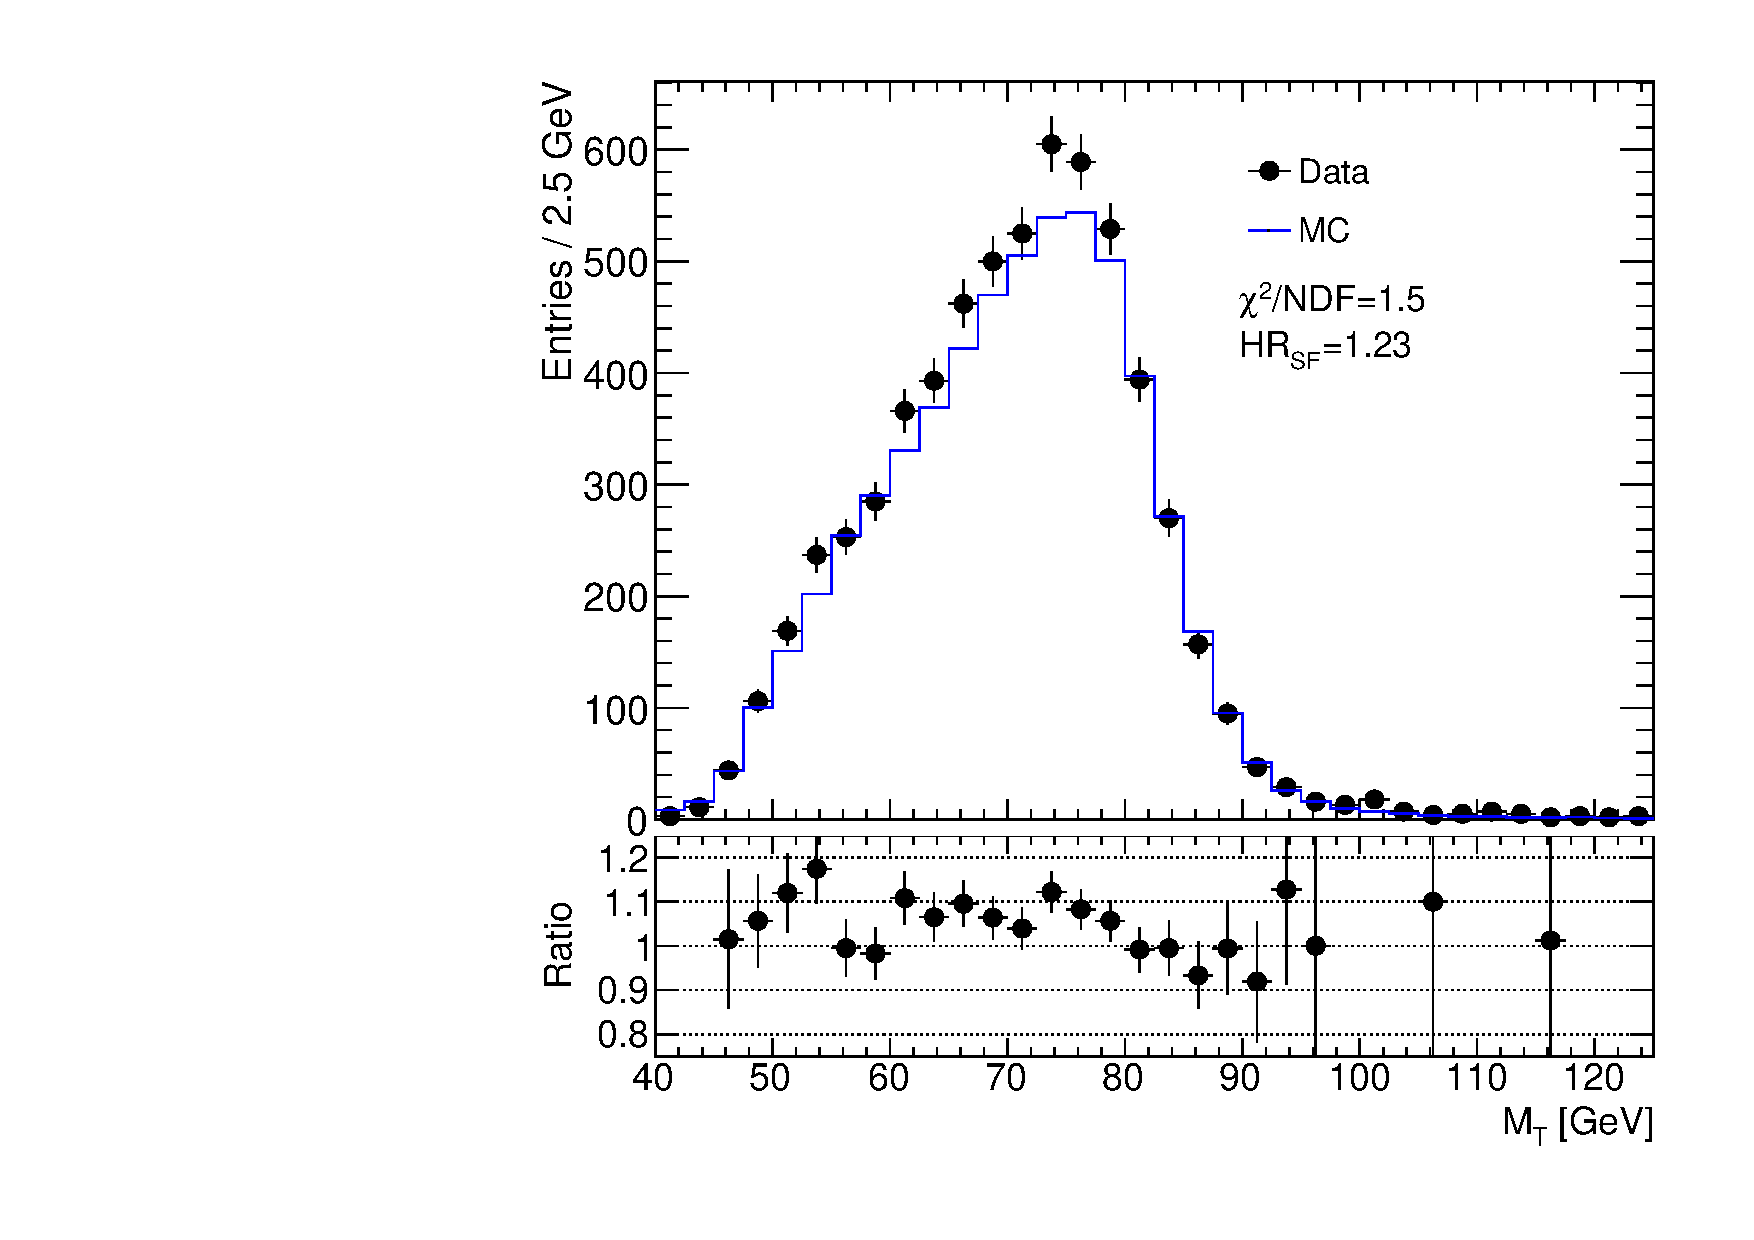
\includegraphics[width=\linewidth]{HadronRecoil/MtWEScale24.pdf} c)}
\endminipage
\caption{Transverse mass distribution from the \wenu selection for different hadronic recoil scales: a) $HR_{SF}$=0.75 b) $HR_{SF}$= 1.1 c) $HR_{SF}$=1.23. The expected contributions from signals and backgrounds are estimated with Monte Carlo simulation, except for a QCD background, that is not included.}
\label{HadronRecoilScaleMtW}
\end{figure}
As it was mentioned before, the hadronic recoil value in Monte Carlo could be shifted in a respect to data because of the mismodelling of underlying event, calorimeter cluster responces, etc. Since the value of hadronic recoil affects the \etmiss distribution this discrepancy should be corrected. It could be done by applying the correction factor $HR_{SF}$ on a hadronic recoil in Monte-Carlo sample as:
\begin{equation}
\upar^{cor}=\upar \cdot HR_{SF},
\end{equation}
where \upar is a parallel component in the respect to the true boson direction of hadronic recoil.

The procedure of hadronic recoil bias determination uses a parameter scan through the wide range of the possible $HR_{SF}$ values. It is assumed, that the "real" value of the bias is corresponding to a best agreement between data and MC and therefore can be obtained through the fit of \chiD of some distribution as:
\begin{equation}\label{eq:chiD}
\chi^2 = \frac{(HR_{SF}-sf_{best})^2}{\sigma_{sf}^2}+\chi^2_0,
\end{equation}
where $sf_{best}$ is the best scale factor,  $\sigma_{sf}$ is a statistical error of this parameter and $\chi^2_0$ is a value of \chiD in a minimum. 

In the following sections methods of hadronic recoil bias determination using W and Z events will be discussed.

\subsection{Bias determination from \mtw distribution}


Since the W boson transverse momentum cannot be measured in two different ways in order to provide the reference for a hadronic recoil scale, determination of the hadronic recoil bias should use the distributions, that  are not sensitive to the true \ptw spectrum, to exclude the effect of possible \ptw mismodelling in MC.  One of the optimal choices is the \mtw distribution. 

The transverse mass distribution for a different correction parameters $HR_{SF}$ is shown on a Fig. \ref{HadronRecoilScaleMtW}. The expected contributions from signal and backgrounds are estimated with Monte Carlo simulation, except for a multijet background, because its shape and number of events depends on a hadronic recoil scale and thus needs to be recalculated for each value of $HR_{SF}$. 

\begin{figure}[!tbp]
\begin{minipage}[h]{0.49\linewidth}
\center{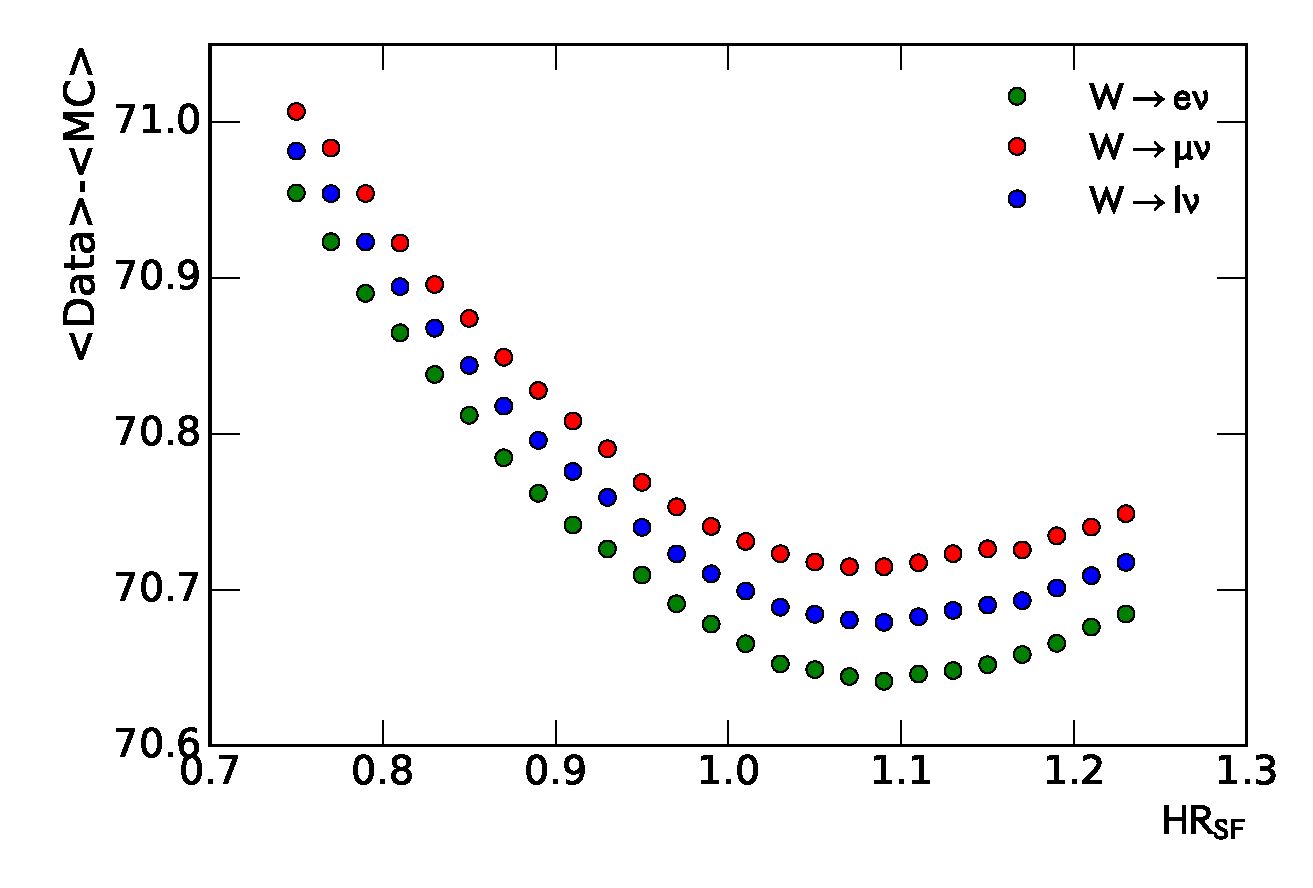
\includegraphics[width=1.\linewidth]{HadronRecoil/MeanAll.pdf} \\ a)}
\end{minipage}
\hfill
\begin{minipage}[h]{0.49\linewidth}
\center{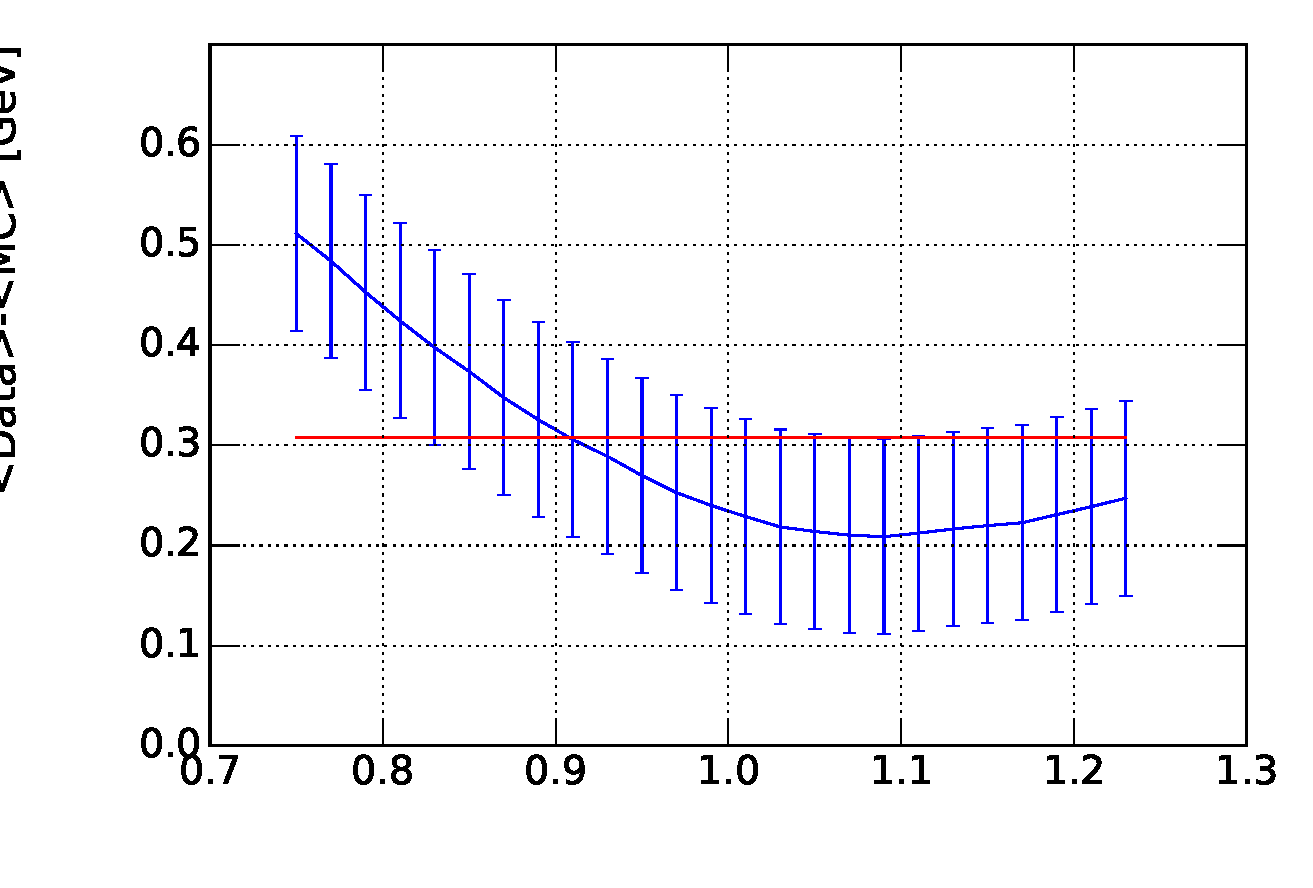
\includegraphics[width=1.\linewidth]{HadronRecoil/MeanCombined.pdf} \\ b)}
\end{minipage}
\caption{Distribution of a difference in a mean transverse mass $<\mtw>$ between data and MC as a function of the hadronic recoil scale $HR_{SF}$ a) for different W boson channels and b) for combined $W \to l \nu$ selection. Errors for each point are calculated as a standard error of mean (Eq. \ref{eq:MeanErr}). Below red line is the 68\% CL on the best $HR_{SF}$ correction factor. The expected contributions from signals and backgrounds are estimated with Monte Carlo simulation, except for a QCD background, that is not included.}
\label{fig:HRBiasMean}
\end{figure}

One of the possible methods to determine the correction factor is to use a difference in the mean of the transverse mass distributions in data and MC (Fig.~\ref{fig:HRBiasMean}). Statistical error on a correction factor is considered a dominating one and estimated as a standard error of a mean $\sigma ( <\mtw> ) $, calculated as:
\begin{equation}\label{eq:MeanErr}
\sigma \Big( <\mtw> \Big) = \frac{\sigma( \mtw )}{\sqrt N},
\end{equation}
where $\sigma(\mtw)$ is a standard deviation of $\mtw$ distribution and N is a total number of events used. The minimal difference is obtained at $HR_{SF}=1.1\pm0.2$. The precision of this method is low, and it is mainly used as a cross-check for other methods. 

\begin{figure}[!tbp]
\begin{minipage}[h]{0.49\linewidth}
\center{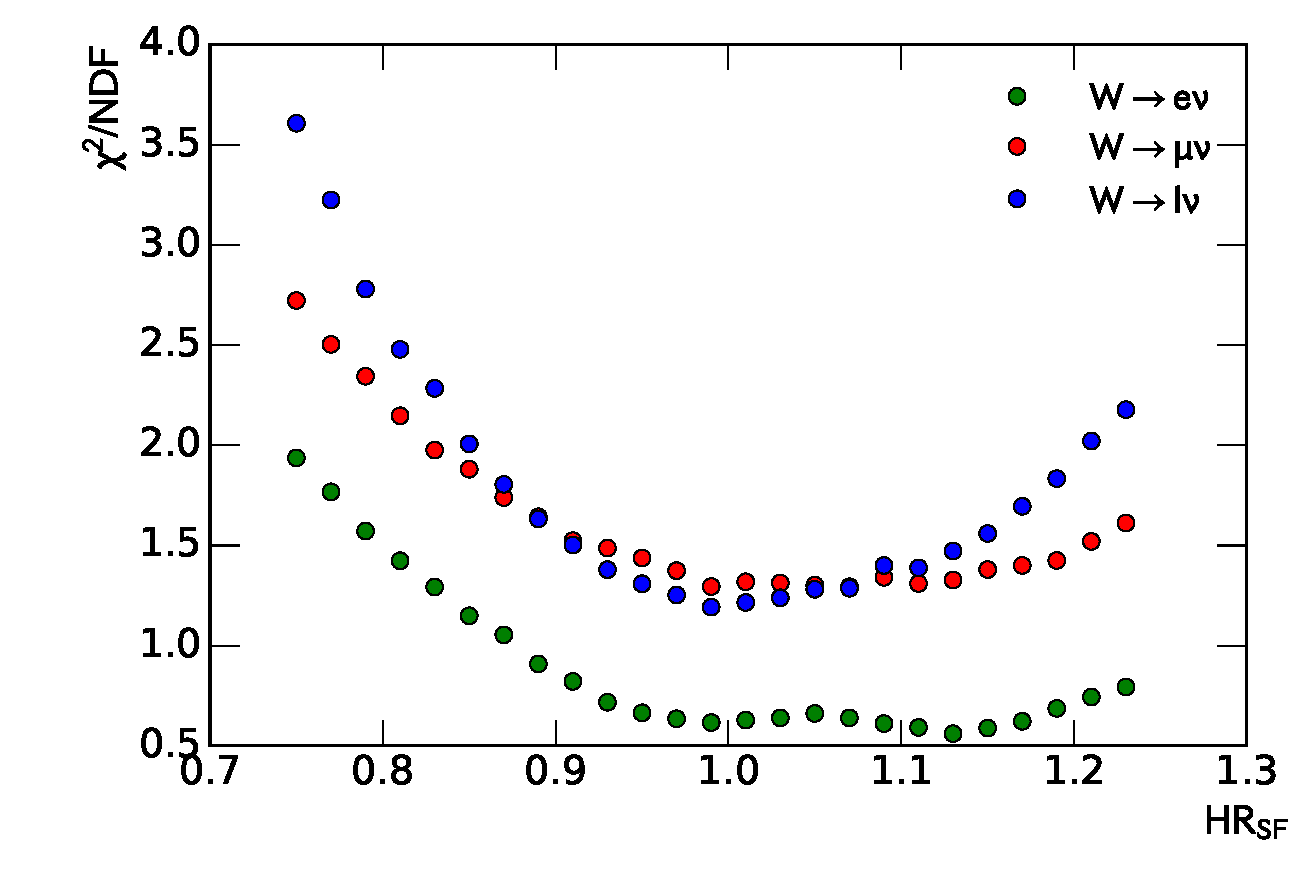
\includegraphics[width=1.\linewidth]{HadronRecoil/chi2AllChannelsMtw.pdf} \\ a)}
\end{minipage}
\hfill
\begin{minipage}[h]{0.49\linewidth}
\center{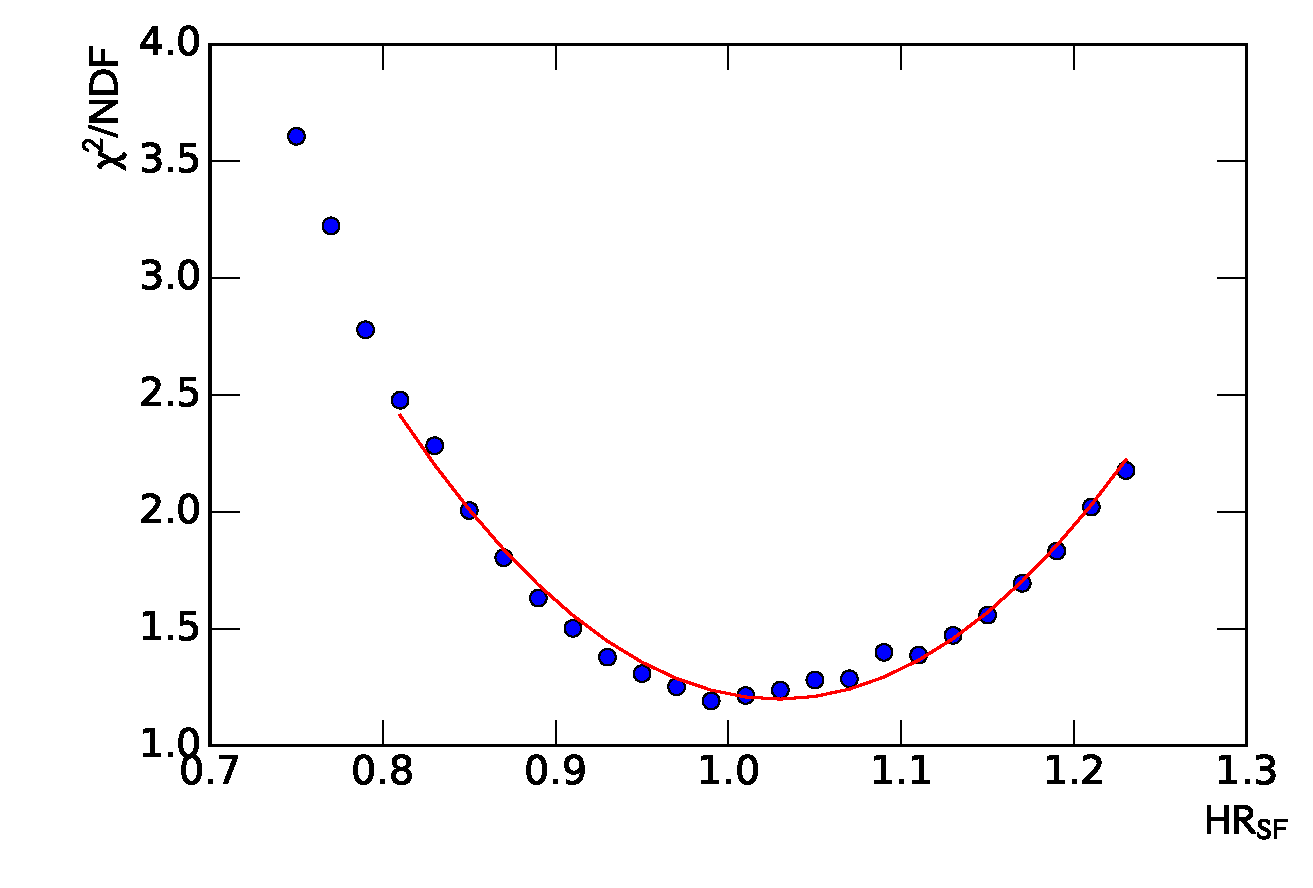
\includegraphics[width=1.\linewidth]{HadronRecoil/chi2TotalMtw.pdf} \\ b)}
\end{minipage}
\caption{Distribution of \chiD/NDF  between data and MC for transverse mass  $<\mtw>$ as a function of hadronic recoil scale $HR_{SF}$ a ) for different W boson channels. 
b) for combined $W \to l \nu$ selection. Fit result is shown by the red line. The expected contributions from signal and backgrounds are estimated with Monte Carlo simulation, except for a QCD background, that is not included.}
\label{mtWChi2}
\end{figure}

\begin{figure}[!tbp]
\centering
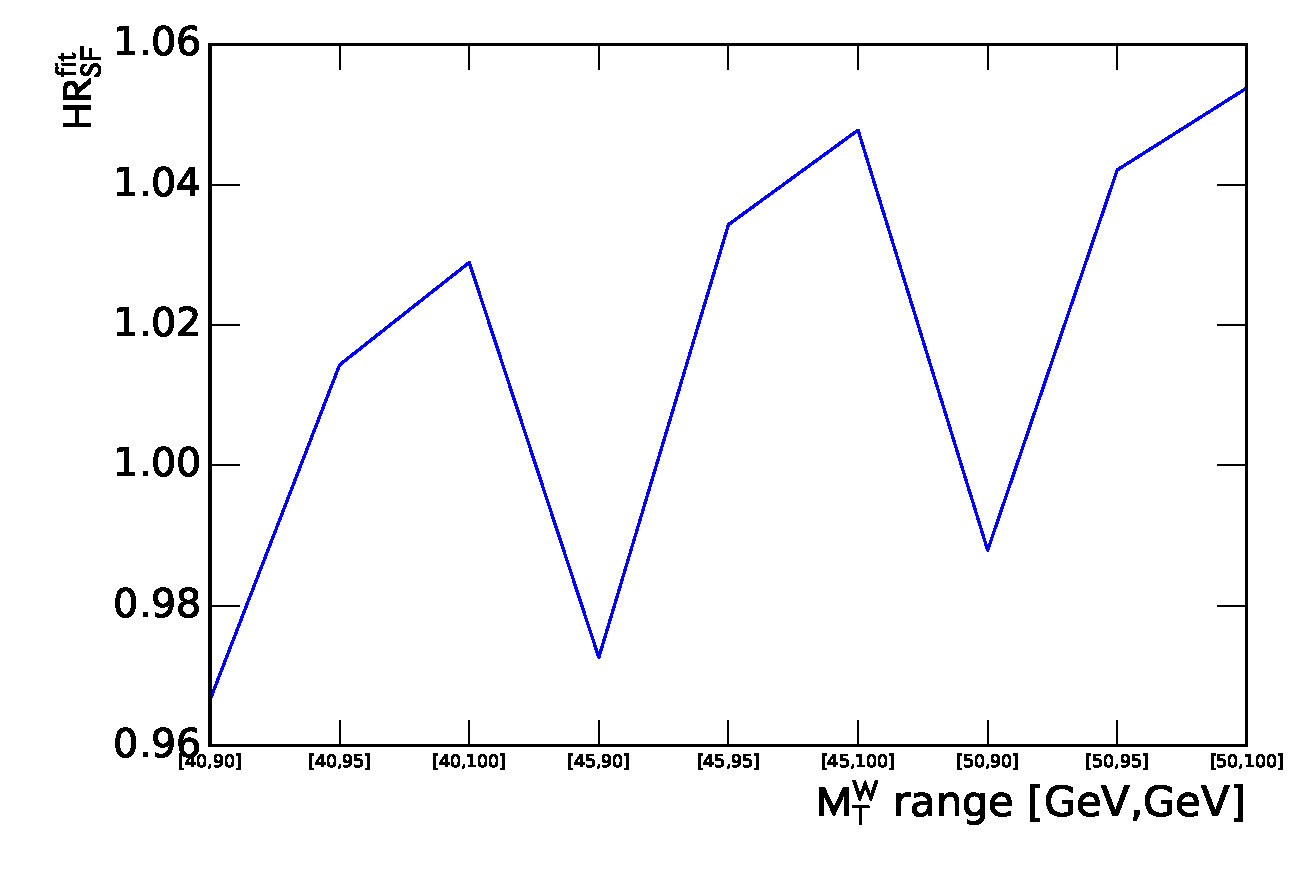
\includegraphics[width=0.5\textwidth]{HadronRecoil/RangeEffect.pdf}
\caption{Values of hadronic recoil biases obtained from the fit for events from combined $W \to l \nu$ selection as a function of fit range. The expected contributions from signals and backgrounds are estimated with Monte Carlo simulation, except for a QCD background, that is not included.}
\label{ScaleMtWRange}
\end{figure}

Distribution of \chiD  for a scan of possible values of $HR_{SF}$ for different W channels is shown in a Fig. \ref{mtWChi2} a). Because of a possible mismodelling of the tail \mtw distribution, events with \mtw > 100 GeV are not included in a \chiD calculation. There is a small peak visible in the \chiD distribution for events from \wenu selection, that can be assumed to come from the missing QCD background contributions. Hadronic recoil bias parameters are determined through the fit of \chiD distribution in combined $W\to l\nu$ channel using the function from Eq.~\ref{eq:chiD}. The resulting bias is $HR_{SF}=1.02$, with the statistical error 0.06. 

Additionally, a cut on \mtw lower value may be used to reduce the multijet background contamination. The \mtw range introduces a source of the systematic uncertainty in the hadronic recoil scale determination. It is estimated by repeating the fit for  different \mtw lower and upper values, as shown in Fig.~\ref{ScaleMtWRange}. Fit range systematic error calculated as an RMS of the obrained values and is 0.03. The final result for this method is $HR_{SF}=1.02\pm0.07$. 


\subsection{Bias determination using \upar distribution}




\begin{figure}[!tbp]
\minipage{0.32\textwidth}
  \center{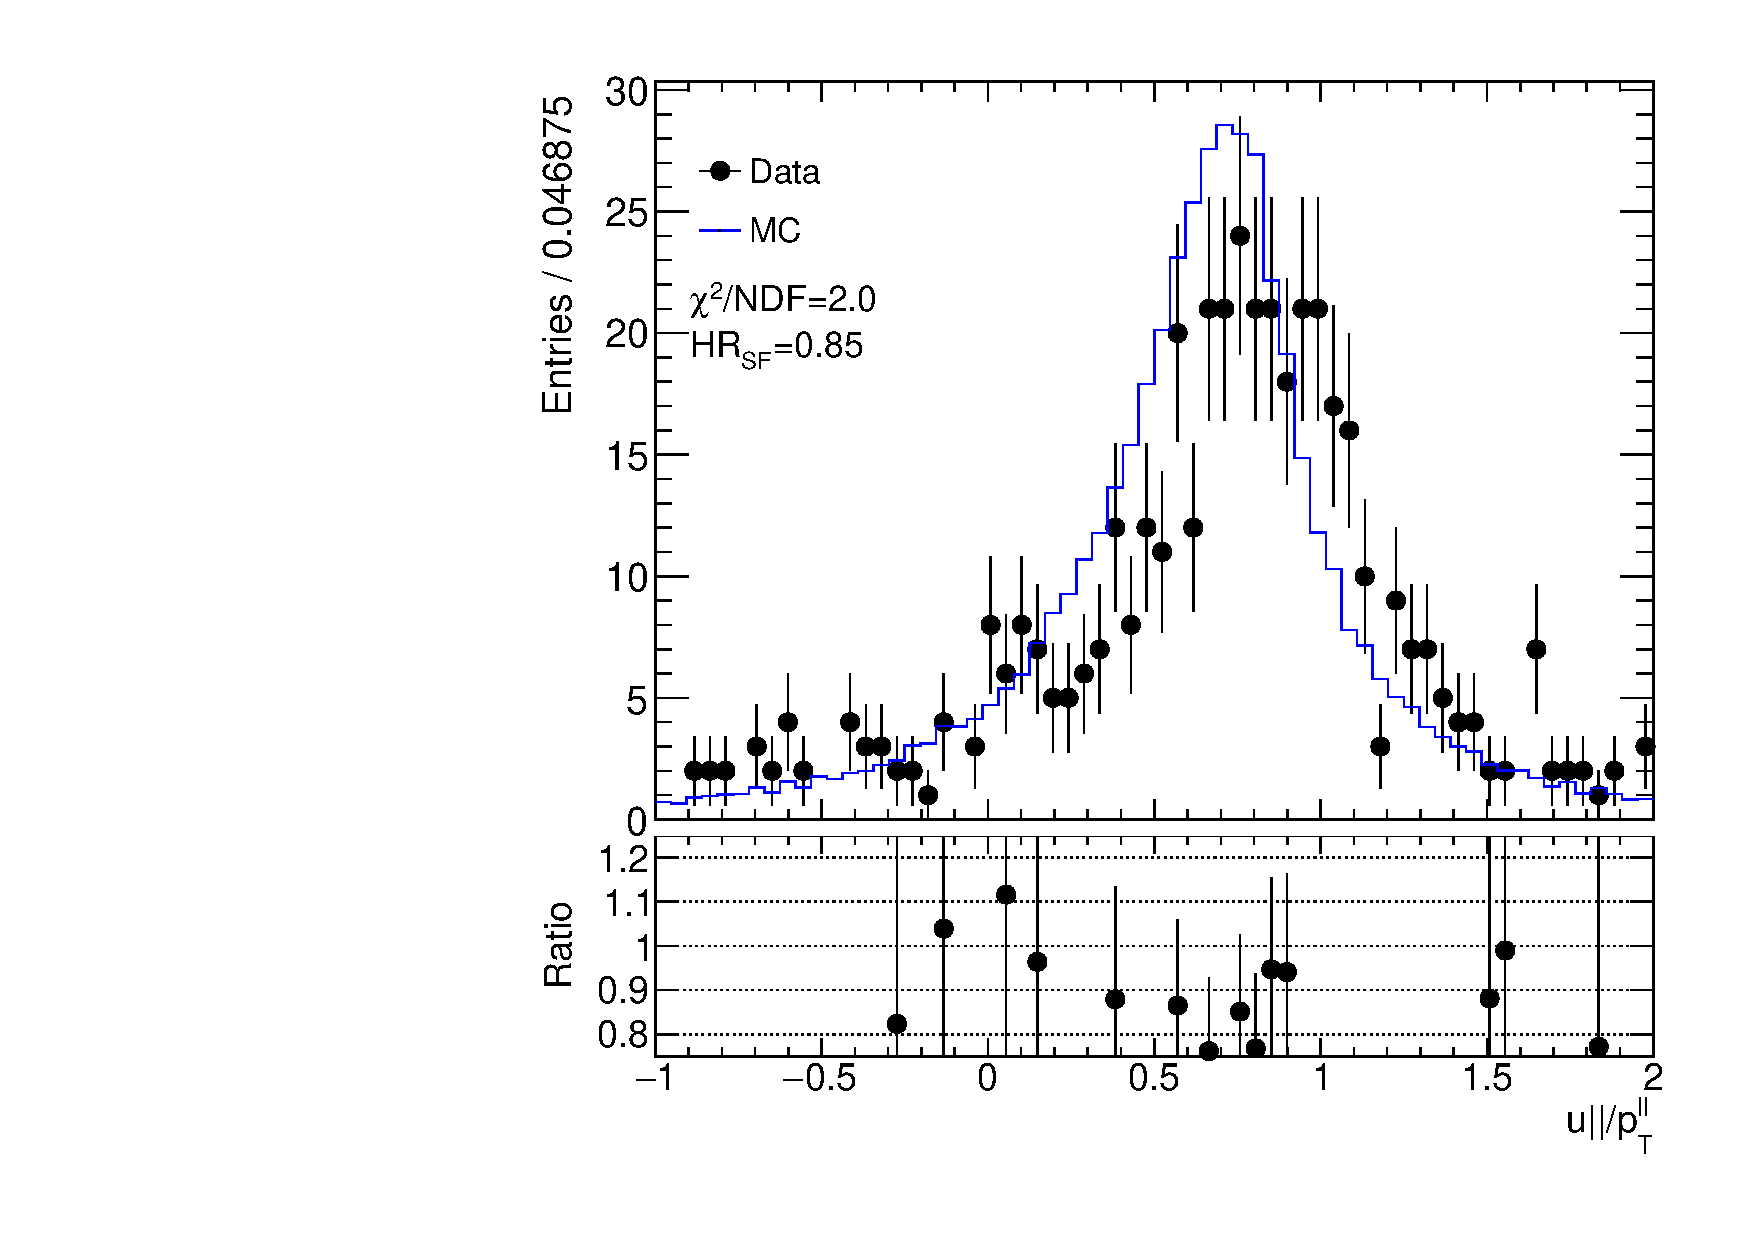
\includegraphics[width=\linewidth]{HadronRecoil/UParEScale5.pdf} a)}
\endminipage\hfill
\minipage{0.32\textwidth}
   \center{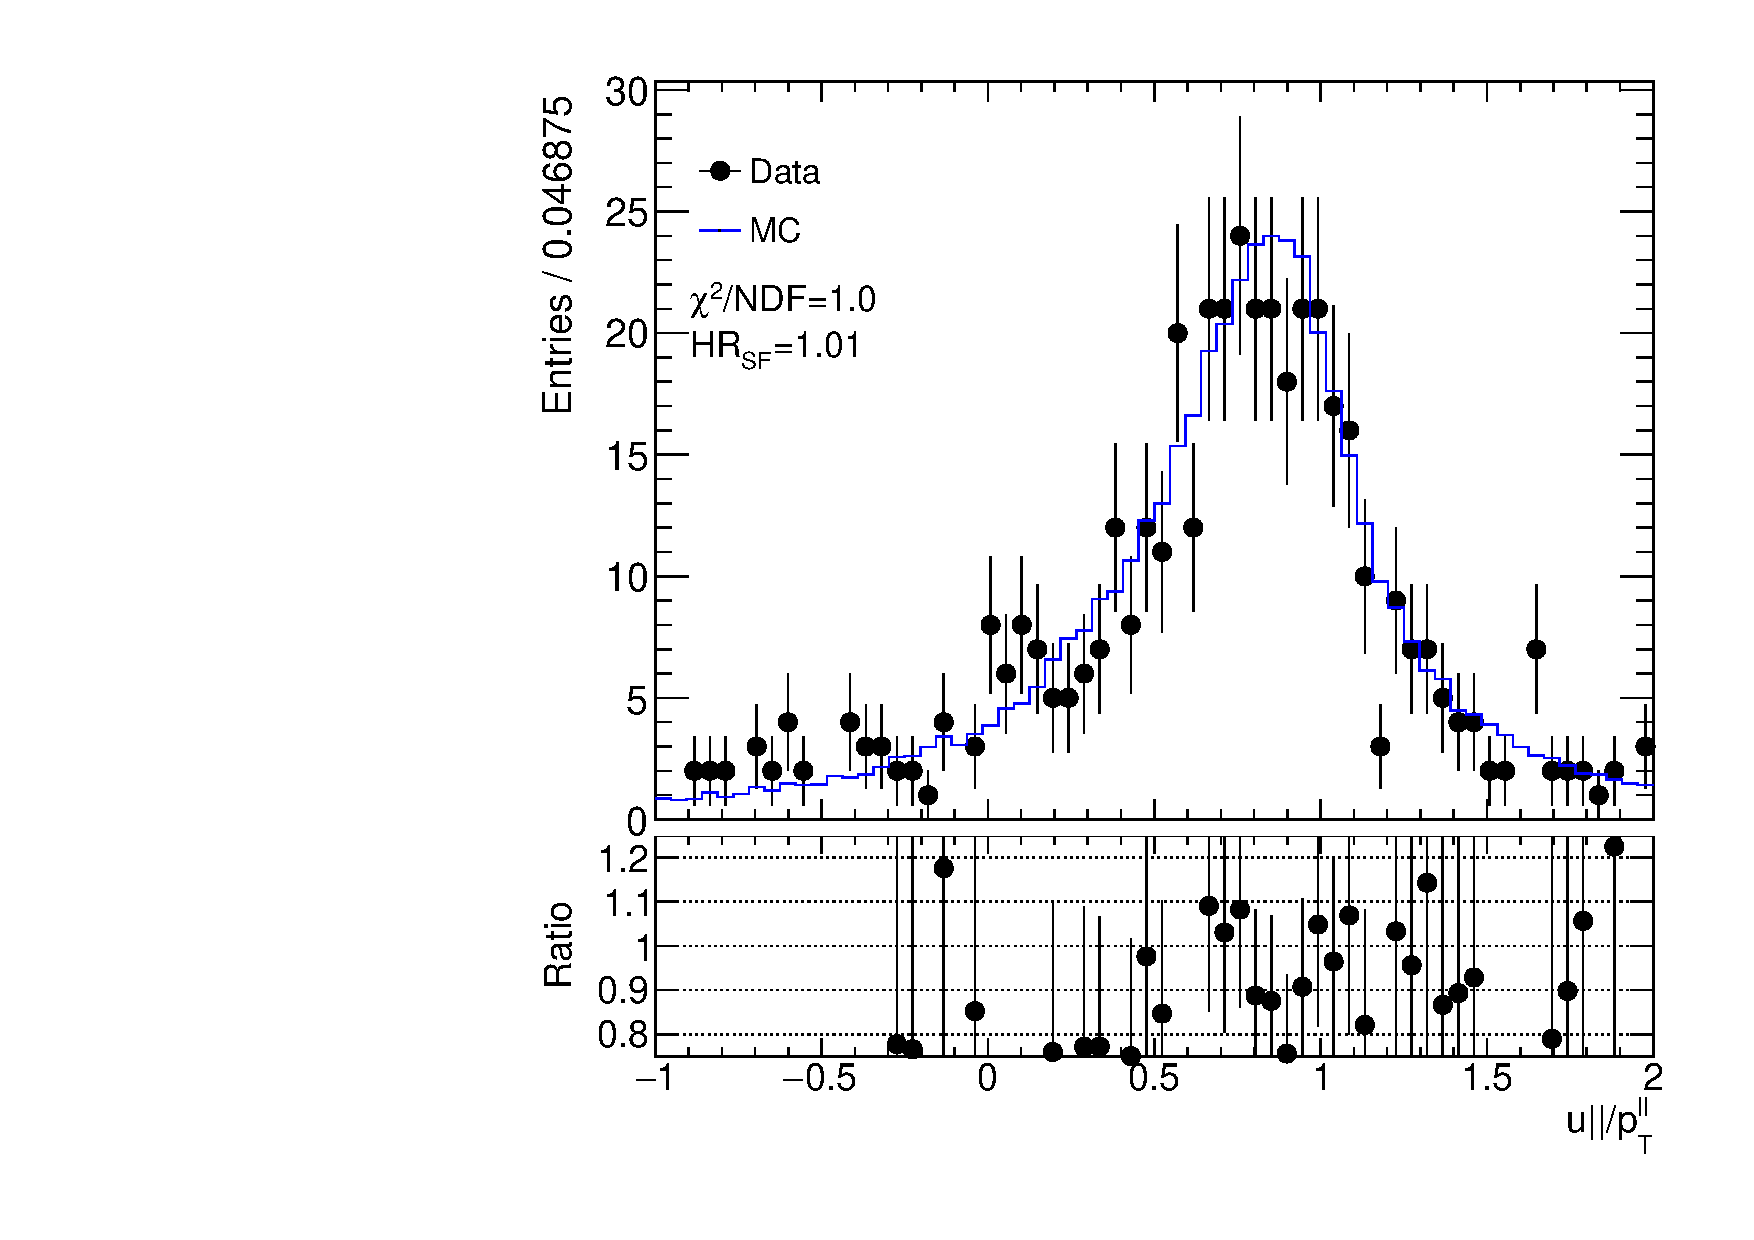
\includegraphics[width=\linewidth]{HadronRecoil/UParEScale13.pdf} b)}
\endminipage\hfill
\minipage{0.32\textwidth}%
   \center{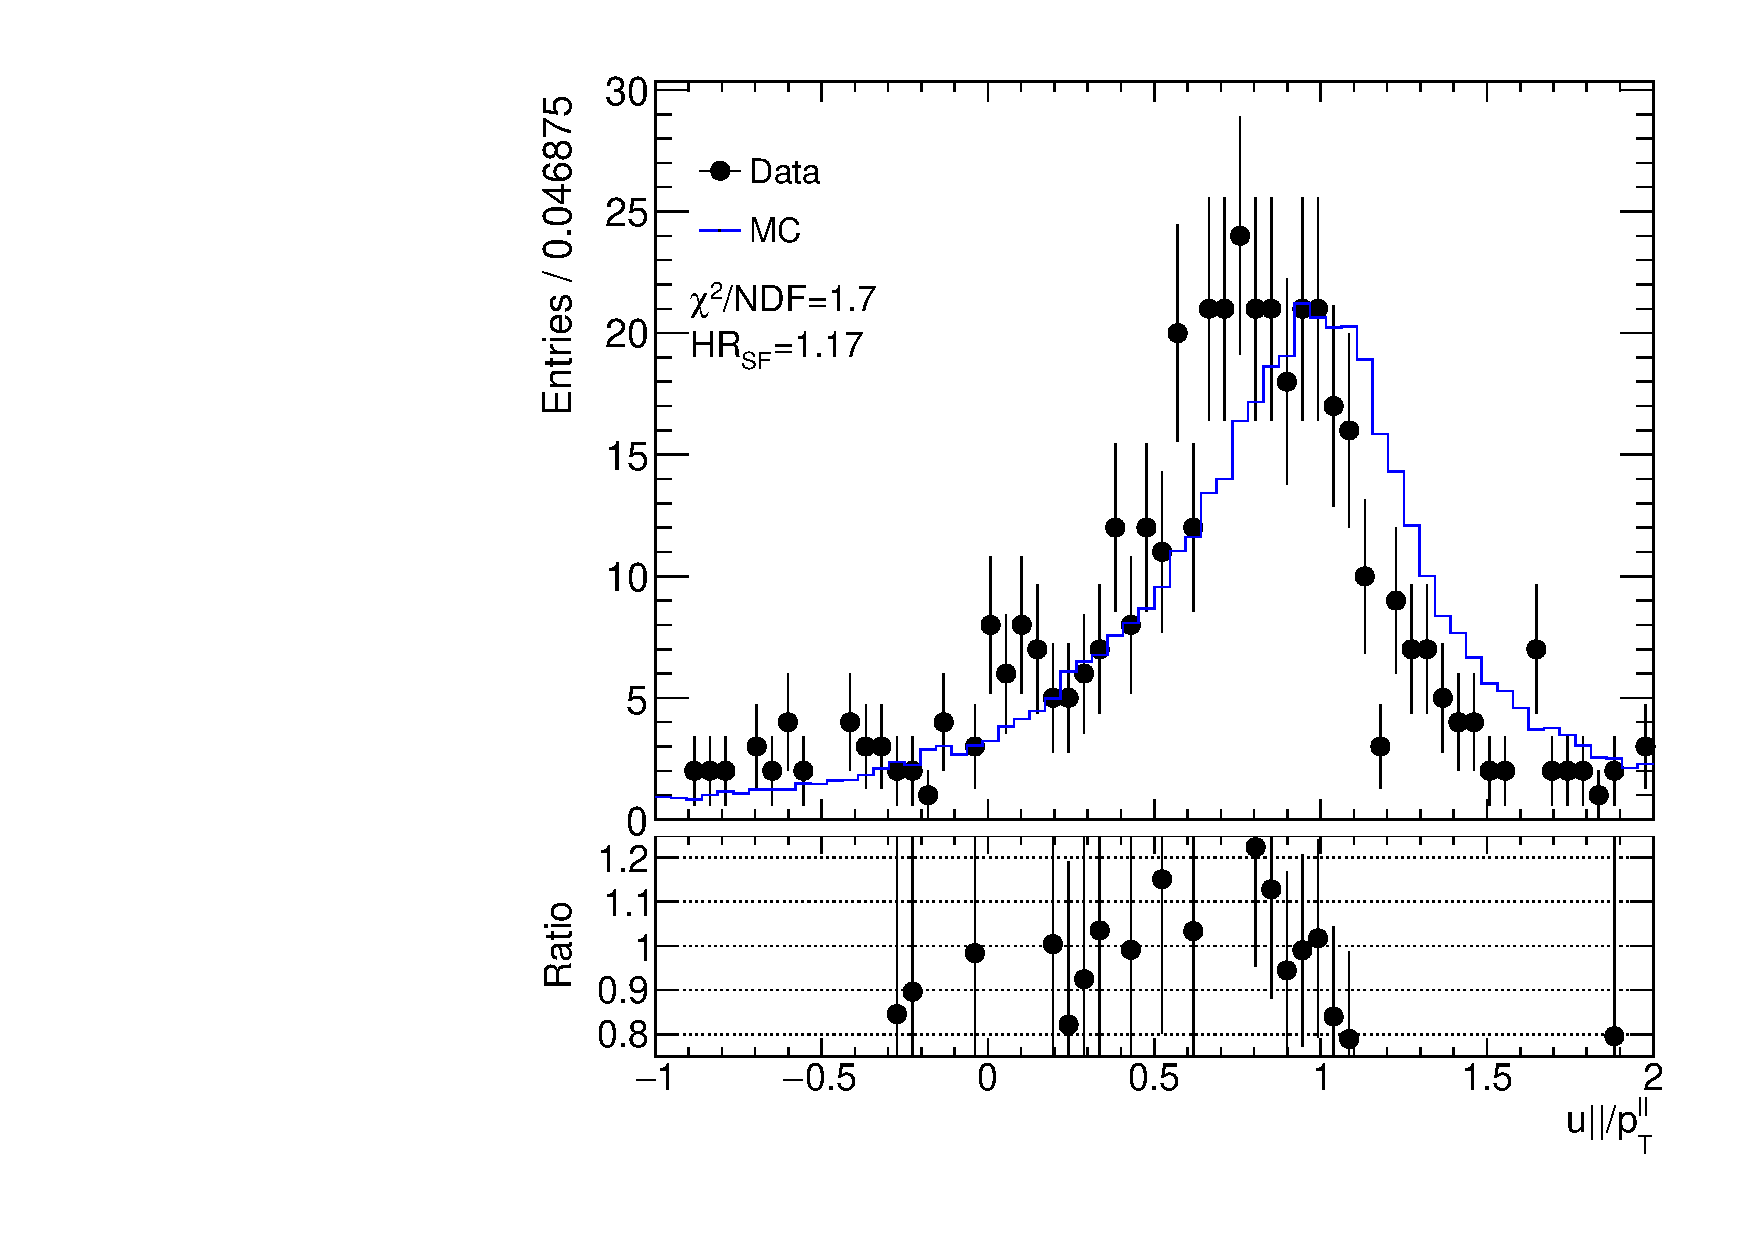
\includegraphics[width=\linewidth]{HadronRecoil/UParEScale21.pdf} c)}
\endminipage
\caption{Parallel hadronic recoil component \upar from the $Z\to ee$ selection for different hadronic recoil scales: a) $HR_{SF}$=0.75 b) $HR_{SF}$= 1.1 c) $HR_{SF}$=1.23. The expected contribution from signal is estimated with Monte Carlo simulation, other background sources are considered negligible.}
\label{HadrRecoil:ZScan}
\end{figure}

\begin{figure}[!tbp]
\begin{minipage}[h]{0.49\linewidth}
\center{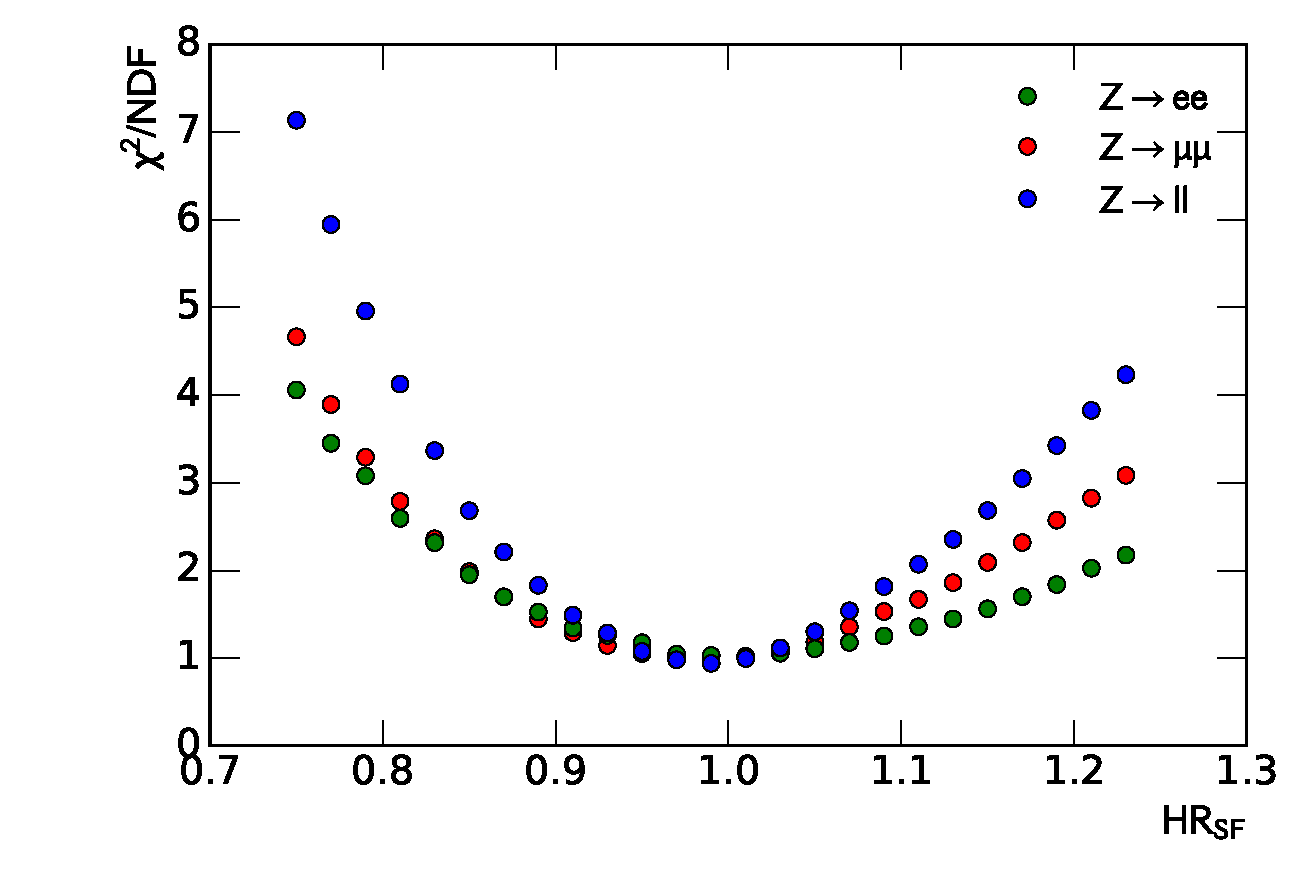
\includegraphics[width=1.\linewidth]{HadronRecoil/chi2Upar.pdf} \\ a)}
\end{minipage}
\hfill
\begin{minipage}[h]{0.49\linewidth}
\center{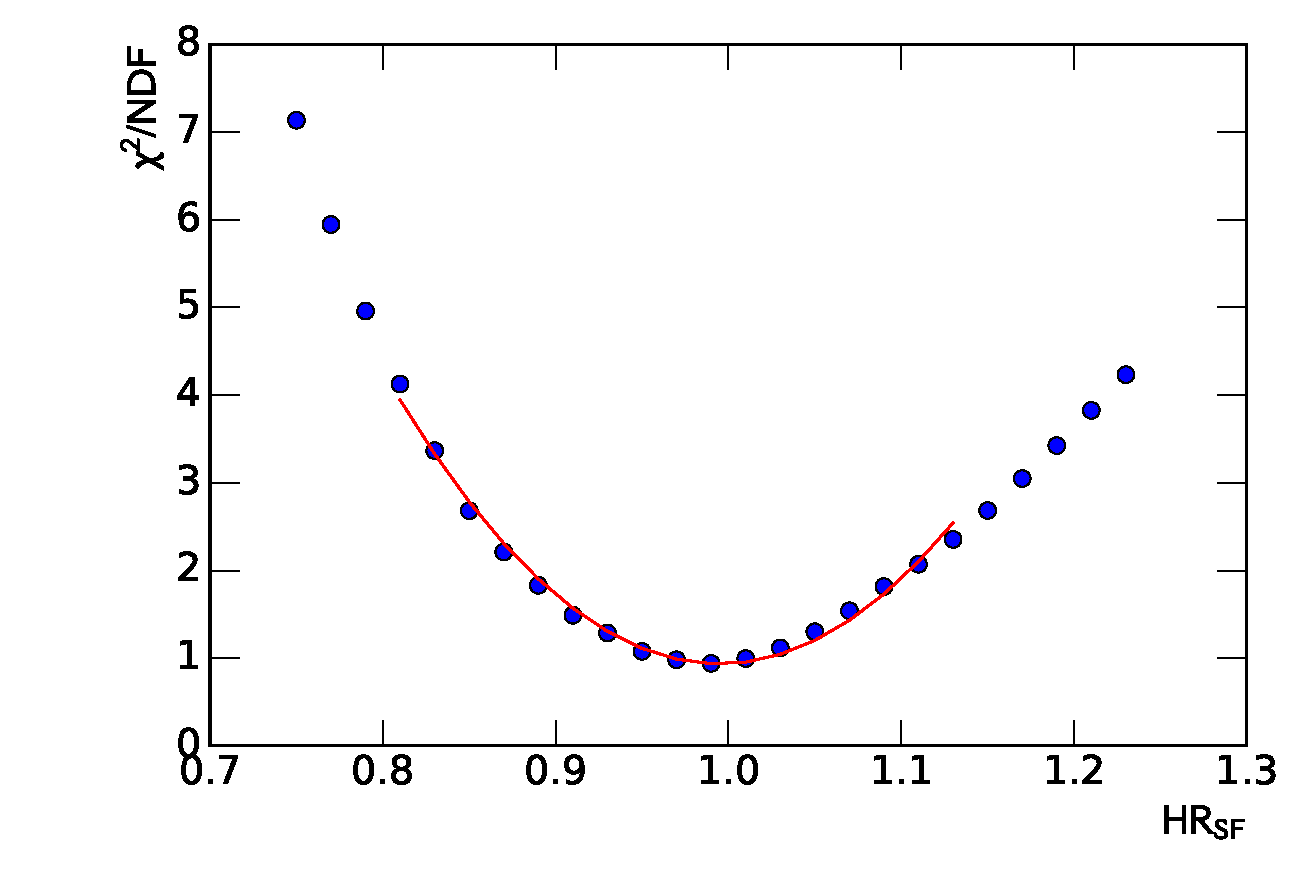
\includegraphics[width=1.\linewidth]{HadronRecoil/chi2UparTot.pdf} \\ b)}
\end{minipage}
\caption{a) Distribution of \chiD  between data and MC for $\frac{\upar}{p_T^{ll}}$ distribution as a function of hadronic recoil scale $HR_{SF}$ for a) different Z boson channels. 
b) for combined $Z \to ll$ selection. Fit results are shown by a red line.The expected contribution from signal is estimated with Monte Carlo simulation, other background sources are considered negligible.}
\label{uPAr}
\end{figure}  
 
Similarly to the W channel, the scale correction in the Z sample can be determined from the $HR_{SF}$ scan of the $\frac{\upar}{p_T^{ll}}$ distribution, as shown in Fig. \ref{HadrRecoil:ZScan}. All of the backgrounds sources are considered negligible in this case. Results of the \chiD test for data and MC in different channel are shown in Fig. \ref{uPAr}. A fit of the combined $Z \to ll$ distribution gives the most precise estimation of the hadronic recoil bias $HR_{SF} = 1.00 \pm 0.01$.  Since there is no choice of the range and dependency on $P_T^{bos}$ modeling, there is just one statistical source of uncertainty.



  
\subsection{Sytematic uncertainty estimation}

\begin{table}[!h]
\caption{Hadronic recoil bias determination results and errors for different methods.}
\label{tab:SFHadronRecoil}
\begin{center}
\begin{tabular}{| l | c | c |}
\hline
Method & SF & error \\
\hline
\hline
Mean $M_T^{W}$ & 1.10 & 0.2\\
$M_T^{W}$ \chiD & 1.01 & 0.07 \\
\upar \chiD & 1.00 & 0.014 \\
\hline
\end{tabular}
\end{center}
\end{table}


Results on a hadronic scale factors and its errors are shown in a Table \ref{tab:SFHadronRecoil}. The results are consistent within one sigma.  As a final result it was decided to choose $HR_{SF}$ determined from $Z\to ll$ selection as the are established with smallest uncertainty/ Scale factors extracted with other methods are used as a cross-check.

Effect of the hadronic recoil bias correction for different bias scale factors presented in Fig. \ref{ris:Cw}. Systematic error, coming from the bias correction is estimated using offset method (see Chap. \ref{chap:Unc}). 

\begin{figure}[!tbp]
\begin{minipage}[h]{0.49\linewidth}
\center{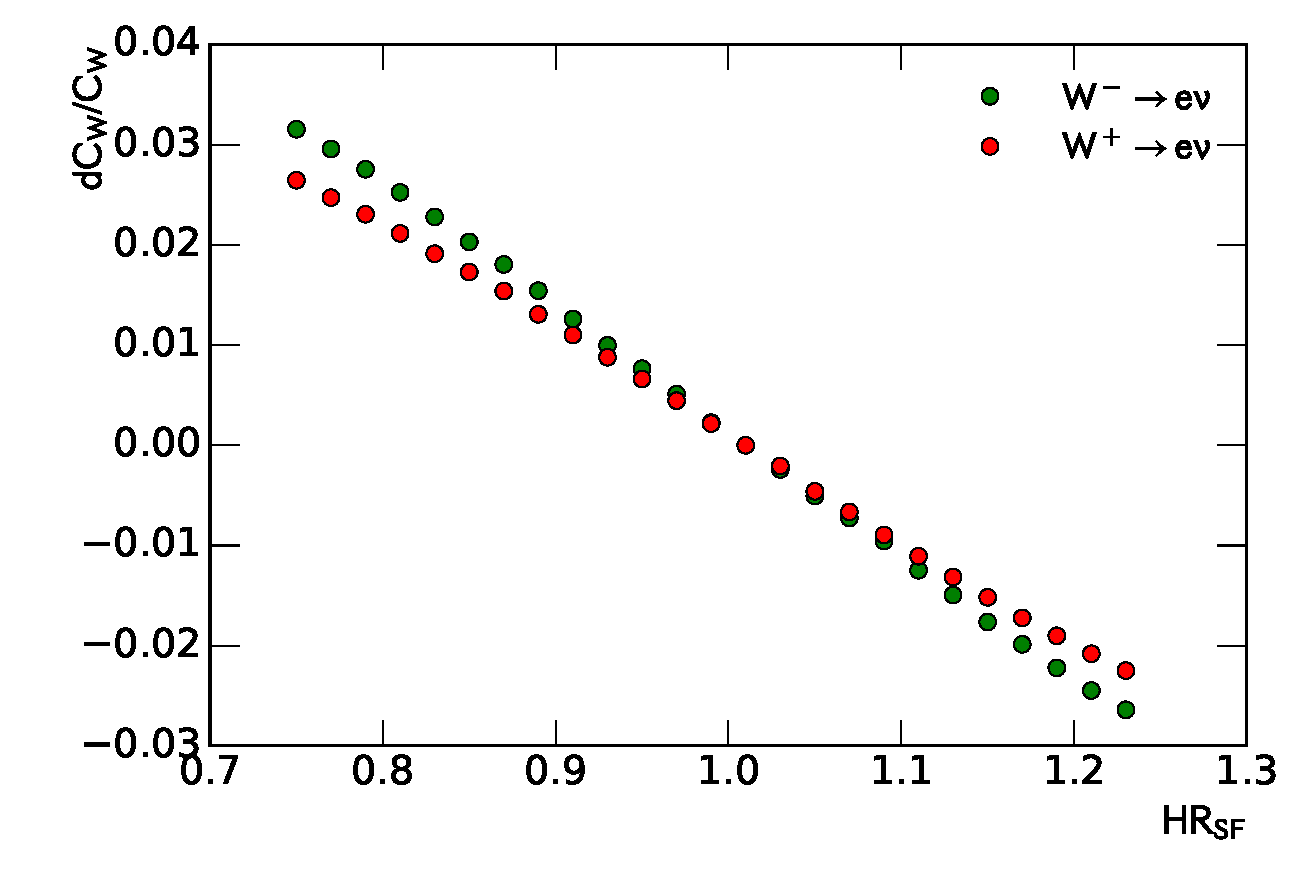
\includegraphics[width=1.\linewidth]{HadronRecoil/CWElectron.pdf} \\ a)}
\end{minipage}
\hfill
\begin{minipage}[h]{0.49\linewidth}
\center{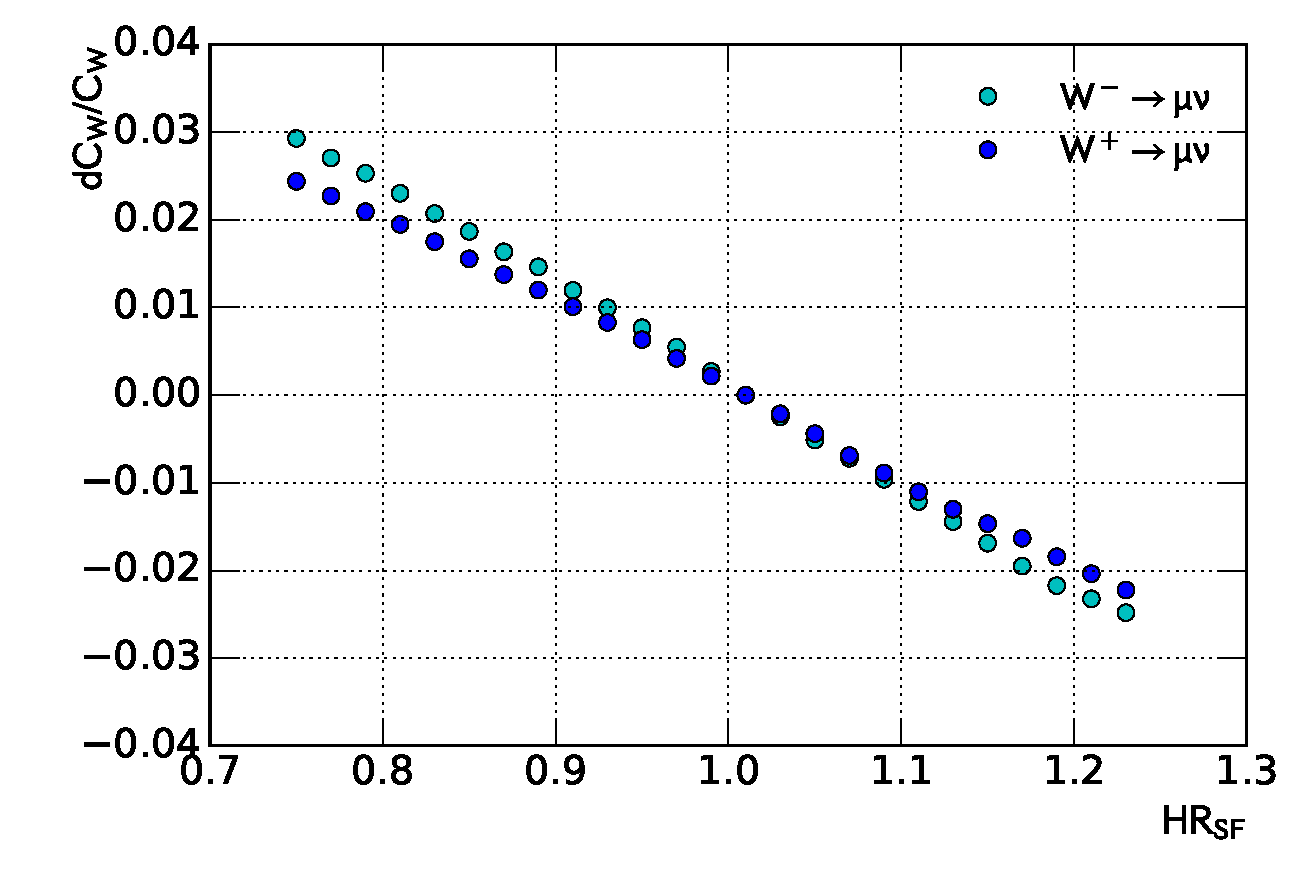
\includegraphics[width=1.\linewidth]{HadronRecoil/CWMuon.pdf} \\ b)}
\end{minipage}
\caption{Effect on a \cw for a different $d\sigma$ for a) \wenu b)\wmunu channel}
\label{ris:Cw}
\end{figure}


\section{Summary on hadronic recoil systematics}
Because of the problems with data vs MC comparison it was decided to use a hadronic recoil algorithm of \etmiss reconstruction. Because of the differences in operation conditions the calibration of hadronic recoil must be determined directly from 2.76 TeV data. The limited statistics of the Z sample does not allow to use the standard procedure, used for the \mtw measurment at 7 TeV, so the new methodology was developed. 

The hadronic recoil calibration can be divided into two parts: the correction of resolution and the bias correction. 
The hadronic recoil resolution have been corrected using the following methods:
\begin{itemize}
\item Event activity correction through the reweighting of \sumet distribution. Different methods of the data/MC ratio parametrization have been developed and showed the consistent result. However, this method gives a unphysical difference between electron and muon channels, that cannot be accounted for the data statistics, so it was decided to drop this method.
\item Smearing correction of the hadronic recoil. This method uses the Z sample to determine the difference in resolutions of the hadronic recoil components. The overall effect of these correction was estimated by repeating the smearing 25 times and consistent between electron and muon channels
\end{itemize}

The bias of hadronic recoil  was estimated on W and Z events using 3 methods:
\begin{itemize}
\item Difference in the mean of the \mtw distributions in data and MC. This method gives the highest uncertainty and used as a cross-check for other results
\item Through the scans of the hadronic recoil scale effect on \chiD in data vs MC \mtw distributions. Error on this method is dominated by the statistics
\item Through the scans of the hadronic recoil scale effect on \chiD in data vs MC $\frac{\upar}{p_T^{ll}}$ distributions. Despite the small size of the Z boson sample, this distribution has the biggest sensitivity to the hadronic recoil scale. It was decided to use this resut and its error as a final result.
\end{itemize}
The results are agreeing between channels within 1 sigma.

The corresponding error sources for the hadronic recoil calibration have been estimated and summarised in the Tab. \ref{tab:SFHadronRecoilBias}. The overall error on \etmiss is around 0.3 \% for all W-boson channels and can be considered a subdominant.

\begin{table}[!tb]
\caption{Hadronic recoil bias systematics for different W boson channels.}
\label{tab:SFHadronRecoilBias}
\begin{center}
\begin{tabular}{| l || c | c | c | c |}
\hline
Systematic source & $W^{+} \to e^{+}\nu$ & $W^{-} \to e^{-}\nu$  & $W^{+} \to \mu^{+}\nu$ & $W^{-} \to \mu^{-}\nu$ \\
\hline
\hline
Hadronic recoil resolution & -0.2\% & -0.11\% & -0.16\% & -0.12\% \\
Hadronic recoil scale &  0.21\% & 0.20\% & 0.23\% & 0.24\% \\
\hline
\end{tabular}
\end{center}
\end{table}